\begin{enumerate}[label=\thesection.\arabic*,ref=\thesection.\theenumi]
\numberwithin{equation}{enumi}
\numberwithin{figure}{enumi}
\numberwithin{table}{enumi}
\item Construct a triangle $ABC$ in which $BC=7cm, \angle{B}=75\degree$ and $AB + AC = 13 cm$.
\label{chapters/9/11/2/1}
%%\documentclass[12pt]{article}
%\usepackage[cmex10]{amsmath}
%\usepackage{amsthm}
%\usepackage{mathrsfs}
%\usepackage{txfonts}
%\usepackage{stfloats}
%\usepackage{bm}
%\usepackage{cite}
%\usepackage{cases}
%\usepackage{subfig}
%\usepackage{longtable}
%\usepackage{multirow}
%\usepackage{enumitem}
%\usepackage{mathtools}
%\usepackage{steinmetz}
%\usepackage{tikz}
%\usepackage{circuitikz}
%\usepackage{verbatim}
%\usepackage{tfrupee}
%\usepackage[breaklinks=true]{hyperref}
%\usepackage{tkz-euclide} % loads  TikZ and tkz-base
%\providecommand{\brak}[1]{\ensuremath{\left(#1\right)}}
%\usepackage{atbegshi}
%\AtBeginDocument{\AtBeginShipoutNext{\AtBeginShipoutDiscard}}
%\usetikzlibrary{calc,math}
%\usepackage{listings}
%    \usepackage{color}                                            %%
%    \usepackage{array}                                            %%
 %   \usepackage{longtable}                                        %%
  %  \usepackage{calc}                                             %%
   % \usepackage{multirow}                                         %%
    %\usepackage{hhline}                                           %%
    %\usepackage{ifthen}                                           %%
  %optionally (for landscape tables embedded in another document): %%
    %\usepackage{lscape}     
%\usepackage{multicol}
%\usepackage{chngcntr}

%\DeclareMathOperator*{\Res}{Res}
%\renewcommand{\baselinestretch}{2}
%\renewcommand\thesection{\arabic{section}}
%\renewcommand\thesubsection{\thesection.\arabic{subsection}}
%\renewcommand\thesubsubsection{\thesubsection.\arabic{subsubsection}}


% correct bad hyphenation here
%\hyphenation{op-tical net-works semi-conduc-tor}
%\def\inputGnumericTable{}                                 %%

%\lstset{
%language=C,
%frame=single, 
%breaklines=true,
%columns=fullflexible
%}
%\begin{document}
%\newtheorem{theorem}{Theorem}[section]
%\newtheorem{problem}{Problem}
%\newtheorem{proposition}{Proposition}[section]
%\newtheorem{lemma}{Lemma}[section]
%\newtheorem{corollary}[theorem]{Corollary}
%\newtheorem{example}{Example}[section]
%\newtheorem{definition}[problem]{Definition}
%\newcommand{\BEQA}{\begin{eqnarray}}
%\newcommand{\EEQA}{\end{eqnarray}}
%\newcommand{\define}{\stackrel{\triangle}{=}}

%\bibliographystyle{IEEEtran}
%\bibliographystyle{ieeetr}
%\providecommand{\mbf}{\mathbf}
%\providecommand{\pr}[1]{\ensuremath{\Pr\left(#1\right)}}
%\providecommand{\qfunc}[1]{\ensuremath{Q\left(#1\right)}}
%\providecommand{\sbrak}[1]{\ensuremath{{}\left[#1\right]}}
%\providecommand{\lsbrak}[1]{\ensuremath{{}\left[#1\right.}}
%\providecommand{\rsbrak}[1]{\ensuremath{{}\left.#1\right]}}
%\providecommand{\brak}[1]{\ensuremath{\left(#1\right)}}
%\providecommand{\lbrak}[1]{\ensuremath{\left(#1\right.}}
%\providecommand{\rbrak}[1]{\ensuremath{\left.#1\right)}}
%\providecommand{\cbrak}[1]{\ensuremath{\left\{#1\right\}}}
%\providecommand{\lcbrak}[1]{\ensuremath{\left\{#1\right.}}
%\providecommand{\rcbrak}[1]{\ensuremath{\left.#1\right\}}}
%\theoremstyle{remark}
%\newtheorem{rem}{Remark}
%\newcommand{\sgn}{\mathop{\mathrm{sgn}}}
%\providecommand{\res}[1]{\Res\displaylimits_{#1}} 
%\providecommand{\mtx}[1]{\mathbf{#1}}
%\providecommand{\fourier}{\overset{\mathcal{F}}{\rightleftharpoons}}
%\providecommand{\system}{\overset{\mathcal{H}}{\longleftrightarrow}}
	%\newcommand{\solution}[2]{\textbf{Solution:}{#1}}
%\newcommand{\solution}{\noindent \textbf{Solution: }}
%\newcommand{\cosec}{\,\text{cosec}\,}
%\providecommand{\dec}[2]{\ensuremath{\overset{#1}{\underset{#2}{\gtrless}}}}
%\newcommand{\myvec}[1]{\ensuremath{\begin{pmatrix}#1\end{pmatrix}}}
%\newcommand{\mydet}[1]{\ensuremath{\begin{vmatrix}#1\end{vmatrix}}}
%\let\vec\mathbf
%\begin{center}
%\title{\textbf{Straight Lines}}
%\date{\vspace{-5ex}} %Not to print date automatically
%\maketitle
%\end{center}
%\setcounter{page}{1}
%\section*{11$^{th}$ Maths - Chapter 10}
%This is Problem-10 from Exercise 10.4
%\begin{enumerate}
%    \item If three lines whose equations are $y=m_1x+c_1$, $y=m_2x+c_2$ and $y=m_3x+c_3$ are concurrent, then show that $m_1(c_2-c_3)+m_2(c_3-c_1)+m_3(c_1-c_2) = 0.$\\
%    \solution 
    Given lines can be written as \begin{align}
       m_1x-y+c_1=0
    \end{align}
    \begin{align}
        m_2x-y+c_2=0
    \end{align}
    \begin{align}
        m_3x-y+c_3=0
        \label{eq:3}
    \end{align}
    
    
   The above lines can be written in the form of \begin{align}
        \Vec{n}^{\top}\Vec{x} = c
    \end{align}
   Therefore,
		\begin{align}
       \myvec{m_1&-1}\vec{x}=c_1
       \label{eq:5}
   \end{align} 
   \begin{align}
       \myvec{m_2&-1}\vec{x}=c_2
       \label{eq:6}
   \end{align}
   \begin{align}
       \myvec{m_3&-1}\vec{x}=c_3
       \label{eq:7}
   \end{align}
   Solving equations \eqref{eq:5}, \eqref{eq:6}and \eqref{eq:7}
		augumented matrix is
 \begin{align}
    \myvec{m_1&-1&c_1\\m_2&-1&c_2\\m_3&-1&c_3}\\
    \xleftrightarrow{R_2 \leftarrow m_1R_2-m_2R_1}
    \myvec{m_1&-1&c_1\\0&m_2-m_1&m_1c_2-m_2c_1\\m_3&-1&c_3}\\
    \xleftrightarrow{R_3 \leftarrow m_1R_3-m_3R_1}
    \myvec{m_1&-1&c_1\\0&m_2-m_1&m_1c_2-m_2c_1\\0&m_3-m_1&m_1c_3-m_3c_1}\\
    \xleftrightarrow{R_3 \leftarrow R_3\frac{m_2-m_1}{m_3-m_1}-R_2}
        \myvec{m_1&-1&c_1\\0&m_2-m_1&m_1c_2-m_2c_1\\0&0&$\brak{m_1c_3-m_3c_1}$$\brak{\frac{m_2-m_1}{m_3-m_1}}$-$\brak{m_1c_2-m_2c_1}$}
\end{align}
Now, for lines to be concurrent, then the third row should be equal to zero. \\

Therefore,
\begin{align}
\brak{m_1c_3-m_3c_1}\brak{\frac{m_2-m_1}{m_3-m_1}}-\brak{m_1c_2-m_2c_1}=0\\
\frac{\brak{m_1c_3-m_3c_1}\brak{m_2-m_1}-\brak{m_1c_2-m_2c_1}\brak{m_3-m_1}}{m_3-m_1}=0\\
\brak{m_1c_3-m_3c_1}\brak{m_2-m_1}-\brak{m_1c_2-m_2c_1}\brak{m_3-m_1}=0\\
m_2c_3-m_1c_3+m_3c_1-m_3c_2+m_1c_2-m_2c_1=0\\
m_1\brak{c_2-c_3}+m_2\brak{c_3-c_1}+m_3\brak{c_1-c_2} = 0
\end{align}
           Hence proved
%\begin{figure}[h]
 %   \centering
  %  \includegraphics[width=\columnwidth]{concurrent-1.png}
   % \caption{Straight Lines}
    %\label{fig:concurrent-1.png}
%\end{figure}
%\end{enumerate}
%\end{document}

%
\item Construct a triangle $ABC$ in which $BC=8cm, \angle{B}=45\degree$ and $AB - AC = 3.5 cm$.
\label{chapters/9/11/2/2}
\\
\solution
\input{chapters/9/11/2/2-new/vector-2.tex}
%
\item Construct a triangle $PQR$ in which $QR=6cm, \angle{Q}=60\degree$ and $PR - PQ = 2cm$.
\label{chapters/9/11/2/3}
%%\documentclass[12pt]{article}
%\usepackage[cmex10]{amsmath}
%\usepackage{amsthm}
%\usepackage{mathrsfs}
%\usepackage{txfonts}
%\usepackage{stfloats}
%\usepackage{bm}
%\usepackage{cite}
%\usepackage{cases}
%\usepackage{subfig}
%\usepackage{longtable}
%\usepackage{multirow}
%\usepackage{enumitem}
%\usepackage{mathtools}
%\usepackage{steinmetz}
%\usepackage{tikz}
%\usepackage{circuitikz}
%\usepackage{verbatim}
%\usepackage{tfrupee}
%\usepackage[breaklinks=true]{hyperref}
%\usepackage{tkz-euclide} % loads  TikZ and tkz-base
%\providecommand{\brak}[1]{\ensuremath{\left(#1\right)}}
%\usepackage{atbegshi}
%\AtBeginDocument{\AtBeginShipoutNext{\AtBeginShipoutDiscard}}
%\usetikzlibrary{calc,math}
%\usepackage{listings}
%    \usepackage{color}                                            %%
%    \usepackage{array}                                            %%
 %   \usepackage{longtable}                                        %%
  %  \usepackage{calc}                                             %%
   % \usepackage{multirow}                                         %%
    %\usepackage{hhline}                                           %%
    %\usepackage{ifthen}                                           %%
  %optionally (for landscape tables embedded in another document): %%
    %\usepackage{lscape}     
%\usepackage{multicol}
%\usepackage{chngcntr}

%\DeclareMathOperator*{\Res}{Res}
%\renewcommand{\baselinestretch}{2}
%\renewcommand\thesection{\arabic{section}}
%\renewcommand\thesubsection{\thesection.\arabic{subsection}}
%\renewcommand\thesubsubsection{\thesubsection.\arabic{subsubsection}}


% correct bad hyphenation here
%\hyphenation{op-tical net-works semi-conduc-tor}
%\def\inputGnumericTable{}                                 %%

%\lstset{
%language=C,
%frame=single, 
%breaklines=true,
%columns=fullflexible
%}
%\begin{document}
%\newtheorem{theorem}{Theorem}[section]
%\newtheorem{problem}{Problem}
%\newtheorem{proposition}{Proposition}[section]
%\newtheorem{lemma}{Lemma}[section]
%\newtheorem{corollary}[theorem]{Corollary}
%\newtheorem{example}{Example}[section]
%\newtheorem{definition}[problem]{Definition}
%\newcommand{\BEQA}{\begin{eqnarray}}
%\newcommand{\EEQA}{\end{eqnarray}}
%\newcommand{\define}{\stackrel{\triangle}{=}}

%\bibliographystyle{IEEEtran}
%\bibliographystyle{ieeetr}
%\providecommand{\mbf}{\mathbf}
%\providecommand{\pr}[1]{\ensuremath{\Pr\left(#1\right)}}
%\providecommand{\qfunc}[1]{\ensuremath{Q\left(#1\right)}}
%\providecommand{\sbrak}[1]{\ensuremath{{}\left[#1\right]}}
%\providecommand{\lsbrak}[1]{\ensuremath{{}\left[#1\right.}}
%\providecommand{\rsbrak}[1]{\ensuremath{{}\left.#1\right]}}
%\providecommand{\brak}[1]{\ensuremath{\left(#1\right)}}
%\providecommand{\lbrak}[1]{\ensuremath{\left(#1\right.}}
%\providecommand{\rbrak}[1]{\ensuremath{\left.#1\right)}}
%\providecommand{\cbrak}[1]{\ensuremath{\left\{#1\right\}}}
%\providecommand{\lcbrak}[1]{\ensuremath{\left\{#1\right.}}
%\providecommand{\rcbrak}[1]{\ensuremath{\left.#1\right\}}}
%\theoremstyle{remark}
%\newtheorem{rem}{Remark}
%\newcommand{\sgn}{\mathop{\mathrm{sgn}}}
%\providecommand{\res}[1]{\Res\displaylimits_{#1}} 
%\providecommand{\mtx}[1]{\mathbf{#1}}
%\providecommand{\fourier}{\overset{\mathcal{F}}{\rightleftharpoons}}
%\providecommand{\system}{\overset{\mathcal{H}}{\longleftrightarrow}}
	%\newcommand{\solution}[2]{\textbf{Solution:}{#1}}
%\newcommand{\solution}{\noindent \textbf{Solution: }}
%\newcommand{\cosec}{\,\text{cosec}\,}
%\providecommand{\dec}[2]{\ensuremath{\overset{#1}{\underset{#2}{\gtrless}}}}
%\newcommand{\myvec}[1]{\ensuremath{\begin{pmatrix}#1\end{pmatrix}}}
%\newcommand{\mydet}[1]{\ensuremath{\begin{vmatrix}#1\end{vmatrix}}}
%\let\vec\mathbf
%\begin{center}
%\title{\textbf{Straight Lines}}
%\date{\vspace{-5ex}} %Not to print date automatically
%\maketitle
%\end{center}
%\setcounter{page}{1}
%\section*{11$^{th}$ Maths - Chapter 10}
%This is Problem-10 from Exercise 10.4
%\begin{enumerate}
%    \item If three lines whose equations are $y=m_1x+c_1$, $y=m_2x+c_2$ and $y=m_3x+c_3$ are concurrent, then show that $m_1(c_2-c_3)+m_2(c_3-c_1)+m_3(c_1-c_2) = 0.$\\
%    \solution 
    Given lines can be written as \begin{align}
       m_1x-y+c_1=0
    \end{align}
    \begin{align}
        m_2x-y+c_2=0
    \end{align}
    \begin{align}
        m_3x-y+c_3=0
        \label{eq:3}
    \end{align}
    
    
   The above lines can be written in the form of \begin{align}
        \Vec{n}^{\top}\Vec{x} = c
    \end{align}
   Therefore,
		\begin{align}
       \myvec{m_1&-1}\vec{x}=c_1
       \label{eq:5}
   \end{align} 
   \begin{align}
       \myvec{m_2&-1}\vec{x}=c_2
       \label{eq:6}
   \end{align}
   \begin{align}
       \myvec{m_3&-1}\vec{x}=c_3
       \label{eq:7}
   \end{align}
   Solving equations \eqref{eq:5}, \eqref{eq:6}and \eqref{eq:7}
		augumented matrix is
 \begin{align}
    \myvec{m_1&-1&c_1\\m_2&-1&c_2\\m_3&-1&c_3}\\
    \xleftrightarrow{R_2 \leftarrow m_1R_2-m_2R_1}
    \myvec{m_1&-1&c_1\\0&m_2-m_1&m_1c_2-m_2c_1\\m_3&-1&c_3}\\
    \xleftrightarrow{R_3 \leftarrow m_1R_3-m_3R_1}
    \myvec{m_1&-1&c_1\\0&m_2-m_1&m_1c_2-m_2c_1\\0&m_3-m_1&m_1c_3-m_3c_1}\\
    \xleftrightarrow{R_3 \leftarrow R_3\frac{m_2-m_1}{m_3-m_1}-R_2}
        \myvec{m_1&-1&c_1\\0&m_2-m_1&m_1c_2-m_2c_1\\0&0&$\brak{m_1c_3-m_3c_1}$$\brak{\frac{m_2-m_1}{m_3-m_1}}$-$\brak{m_1c_2-m_2c_1}$}
\end{align}
Now, for lines to be concurrent, then the third row should be equal to zero. \\

Therefore,
\begin{align}
\brak{m_1c_3-m_3c_1}\brak{\frac{m_2-m_1}{m_3-m_1}}-\brak{m_1c_2-m_2c_1}=0\\
\frac{\brak{m_1c_3-m_3c_1}\brak{m_2-m_1}-\brak{m_1c_2-m_2c_1}\brak{m_3-m_1}}{m_3-m_1}=0\\
\brak{m_1c_3-m_3c_1}\brak{m_2-m_1}-\brak{m_1c_2-m_2c_1}\brak{m_3-m_1}=0\\
m_2c_3-m_1c_3+m_3c_1-m_3c_2+m_1c_2-m_2c_1=0\\
m_1\brak{c_2-c_3}+m_2\brak{c_3-c_1}+m_3\brak{c_1-c_2} = 0
\end{align}
           Hence proved
%\begin{figure}[h]
 %   \centering
  %  \includegraphics[width=\columnwidth]{concurrent-1.png}
   % \caption{Straight Lines}
    %\label{fig:concurrent-1.png}
%\end{figure}
%\end{enumerate}
%\end{document}

%
\item Construct a triangle $XYZ$ in which $\angle{Y}=30\degree, \angle{Z}=90\degree$ and  $XY+YZ+ZX=11cm$.
\label{chapters/9/11/2/4}
%%\documentclass[12pt]{article}
%\usepackage[cmex10]{amsmath}
%\usepackage{amsthm}
%\usepackage{mathrsfs}
%\usepackage{txfonts}
%\usepackage{stfloats}
%\usepackage{bm}
%\usepackage{cite}
%\usepackage{cases}
%\usepackage{subfig}
%\usepackage{longtable}
%\usepackage{multirow}
%\usepackage{enumitem}
%\usepackage{mathtools}
%\usepackage{steinmetz}
%\usepackage{tikz}
%\usepackage{circuitikz}
%\usepackage{verbatim}
%\usepackage{tfrupee}
%\usepackage[breaklinks=true]{hyperref}
%\usepackage{tkz-euclide} % loads  TikZ and tkz-base
%\providecommand{\brak}[1]{\ensuremath{\left(#1\right)}}
%\usepackage{atbegshi}
%\AtBeginDocument{\AtBeginShipoutNext{\AtBeginShipoutDiscard}}
%\usetikzlibrary{calc,math}
%\usepackage{listings}
%    \usepackage{color}                                            %%
%    \usepackage{array}                                            %%
 %   \usepackage{longtable}                                        %%
  %  \usepackage{calc}                                             %%
   % \usepackage{multirow}                                         %%
    %\usepackage{hhline}                                           %%
    %\usepackage{ifthen}                                           %%
  %optionally (for landscape tables embedded in another document): %%
    %\usepackage{lscape}     
%\usepackage{multicol}
%\usepackage{chngcntr}

%\DeclareMathOperator*{\Res}{Res}
%\renewcommand{\baselinestretch}{2}
%\renewcommand\thesection{\arabic{section}}
%\renewcommand\thesubsection{\thesection.\arabic{subsection}}
%\renewcommand\thesubsubsection{\thesubsection.\arabic{subsubsection}}


% correct bad hyphenation here
%\hyphenation{op-tical net-works semi-conduc-tor}
%\def\inputGnumericTable{}                                 %%

%\lstset{
%language=C,
%frame=single, 
%breaklines=true,
%columns=fullflexible
%}
%\begin{document}
%\newtheorem{theorem}{Theorem}[section]
%\newtheorem{problem}{Problem}
%\newtheorem{proposition}{Proposition}[section]
%\newtheorem{lemma}{Lemma}[section]
%\newtheorem{corollary}[theorem]{Corollary}
%\newtheorem{example}{Example}[section]
%\newtheorem{definition}[problem]{Definition}
%\newcommand{\BEQA}{\begin{eqnarray}}
%\newcommand{\EEQA}{\end{eqnarray}}
%\newcommand{\define}{\stackrel{\triangle}{=}}

%\bibliographystyle{IEEEtran}
%\bibliographystyle{ieeetr}
%\providecommand{\mbf}{\mathbf}
%\providecommand{\pr}[1]{\ensuremath{\Pr\left(#1\right)}}
%\providecommand{\qfunc}[1]{\ensuremath{Q\left(#1\right)}}
%\providecommand{\sbrak}[1]{\ensuremath{{}\left[#1\right]}}
%\providecommand{\lsbrak}[1]{\ensuremath{{}\left[#1\right.}}
%\providecommand{\rsbrak}[1]{\ensuremath{{}\left.#1\right]}}
%\providecommand{\brak}[1]{\ensuremath{\left(#1\right)}}
%\providecommand{\lbrak}[1]{\ensuremath{\left(#1\right.}}
%\providecommand{\rbrak}[1]{\ensuremath{\left.#1\right)}}
%\providecommand{\cbrak}[1]{\ensuremath{\left\{#1\right\}}}
%\providecommand{\lcbrak}[1]{\ensuremath{\left\{#1\right.}}
%\providecommand{\rcbrak}[1]{\ensuremath{\left.#1\right\}}}
%\theoremstyle{remark}
%\newtheorem{rem}{Remark}
%\newcommand{\sgn}{\mathop{\mathrm{sgn}}}
%\providecommand{\res}[1]{\Res\displaylimits_{#1}} 
%\providecommand{\mtx}[1]{\mathbf{#1}}
%\providecommand{\fourier}{\overset{\mathcal{F}}{\rightleftharpoons}}
%\providecommand{\system}{\overset{\mathcal{H}}{\longleftrightarrow}}
	%\newcommand{\solution}[2]{\textbf{Solution:}{#1}}
%\newcommand{\solution}{\noindent \textbf{Solution: }}
%\newcommand{\cosec}{\,\text{cosec}\,}
%\providecommand{\dec}[2]{\ensuremath{\overset{#1}{\underset{#2}{\gtrless}}}}
%\newcommand{\myvec}[1]{\ensuremath{\begin{pmatrix}#1\end{pmatrix}}}
%\newcommand{\mydet}[1]{\ensuremath{\begin{vmatrix}#1\end{vmatrix}}}
%\let\vec\mathbf
%\begin{center}
%\title{\textbf{Straight Lines}}
%\date{\vspace{-5ex}} %Not to print date automatically
%\maketitle
%\end{center}
%\setcounter{page}{1}
%\section*{11$^{th}$ Maths - Chapter 10}
%This is Problem-10 from Exercise 10.4
%\begin{enumerate}
%    \item If three lines whose equations are $y=m_1x+c_1$, $y=m_2x+c_2$ and $y=m_3x+c_3$ are concurrent, then show that $m_1(c_2-c_3)+m_2(c_3-c_1)+m_3(c_1-c_2) = 0.$\\
%    \solution 
    Given lines can be written as \begin{align}
       m_1x-y+c_1=0
    \end{align}
    \begin{align}
        m_2x-y+c_2=0
    \end{align}
    \begin{align}
        m_3x-y+c_3=0
        \label{eq:3}
    \end{align}
    
    
   The above lines can be written in the form of \begin{align}
        \Vec{n}^{\top}\Vec{x} = c
    \end{align}
   Therefore,
		\begin{align}
       \myvec{m_1&-1}\vec{x}=c_1
       \label{eq:5}
   \end{align} 
   \begin{align}
       \myvec{m_2&-1}\vec{x}=c_2
       \label{eq:6}
   \end{align}
   \begin{align}
       \myvec{m_3&-1}\vec{x}=c_3
       \label{eq:7}
   \end{align}
   Solving equations \eqref{eq:5}, \eqref{eq:6}and \eqref{eq:7}
		augumented matrix is
 \begin{align}
    \myvec{m_1&-1&c_1\\m_2&-1&c_2\\m_3&-1&c_3}\\
    \xleftrightarrow{R_2 \leftarrow m_1R_2-m_2R_1}
    \myvec{m_1&-1&c_1\\0&m_2-m_1&m_1c_2-m_2c_1\\m_3&-1&c_3}\\
    \xleftrightarrow{R_3 \leftarrow m_1R_3-m_3R_1}
    \myvec{m_1&-1&c_1\\0&m_2-m_1&m_1c_2-m_2c_1\\0&m_3-m_1&m_1c_3-m_3c_1}\\
    \xleftrightarrow{R_3 \leftarrow R_3\frac{m_2-m_1}{m_3-m_1}-R_2}
        \myvec{m_1&-1&c_1\\0&m_2-m_1&m_1c_2-m_2c_1\\0&0&$\brak{m_1c_3-m_3c_1}$$\brak{\frac{m_2-m_1}{m_3-m_1}}$-$\brak{m_1c_2-m_2c_1}$}
\end{align}
Now, for lines to be concurrent, then the third row should be equal to zero. \\

Therefore,
\begin{align}
\brak{m_1c_3-m_3c_1}\brak{\frac{m_2-m_1}{m_3-m_1}}-\brak{m_1c_2-m_2c_1}=0\\
\frac{\brak{m_1c_3-m_3c_1}\brak{m_2-m_1}-\brak{m_1c_2-m_2c_1}\brak{m_3-m_1}}{m_3-m_1}=0\\
\brak{m_1c_3-m_3c_1}\brak{m_2-m_1}-\brak{m_1c_2-m_2c_1}\brak{m_3-m_1}=0\\
m_2c_3-m_1c_3+m_3c_1-m_3c_2+m_1c_2-m_2c_1=0\\
m_1\brak{c_2-c_3}+m_2\brak{c_3-c_1}+m_3\brak{c_1-c_2} = 0
\end{align}
           Hence proved
%\begin{figure}[h]
 %   \centering
  %  \includegraphics[width=\columnwidth]{concurrent-1.png}
   % \caption{Straight Lines}
    %\label{fig:concurrent-1.png}
%\end{figure}
%\end{enumerate}
%\end{document}

%
\item Construct a right triangle whose base is 12cm and sum of its hypotenuse and other side is 18cm.
\label{chapters/9/11/2/5}
%%\documentclass[12pt]{article}
%\usepackage[cmex10]{amsmath}
%\usepackage{amsthm}
%\usepackage{mathrsfs}
%\usepackage{txfonts}
%\usepackage{stfloats}
%\usepackage{bm}
%\usepackage{cite}
%\usepackage{cases}
%\usepackage{subfig}
%\usepackage{longtable}
%\usepackage{multirow}
%\usepackage{enumitem}
%\usepackage{mathtools}
%\usepackage{steinmetz}
%\usepackage{tikz}
%\usepackage{circuitikz}
%\usepackage{verbatim}
%\usepackage{tfrupee}
%\usepackage[breaklinks=true]{hyperref}
%\usepackage{tkz-euclide} % loads  TikZ and tkz-base
%\providecommand{\brak}[1]{\ensuremath{\left(#1\right)}}
%\usepackage{atbegshi}
%\AtBeginDocument{\AtBeginShipoutNext{\AtBeginShipoutDiscard}}
%\usetikzlibrary{calc,math}
%\usepackage{listings}
%    \usepackage{color}                                            %%
%    \usepackage{array}                                            %%
 %   \usepackage{longtable}                                        %%
  %  \usepackage{calc}                                             %%
   % \usepackage{multirow}                                         %%
    %\usepackage{hhline}                                           %%
    %\usepackage{ifthen}                                           %%
  %optionally (for landscape tables embedded in another document): %%
    %\usepackage{lscape}     
%\usepackage{multicol}
%\usepackage{chngcntr}

%\DeclareMathOperator*{\Res}{Res}
%\renewcommand{\baselinestretch}{2}
%\renewcommand\thesection{\arabic{section}}
%\renewcommand\thesubsection{\thesection.\arabic{subsection}}
%\renewcommand\thesubsubsection{\thesubsection.\arabic{subsubsection}}


% correct bad hyphenation here
%\hyphenation{op-tical net-works semi-conduc-tor}
%\def\inputGnumericTable{}                                 %%

%\lstset{
%language=C,
%frame=single, 
%breaklines=true,
%columns=fullflexible
%}
%\begin{document}
%\newtheorem{theorem}{Theorem}[section]
%\newtheorem{problem}{Problem}
%\newtheorem{proposition}{Proposition}[section]
%\newtheorem{lemma}{Lemma}[section]
%\newtheorem{corollary}[theorem]{Corollary}
%\newtheorem{example}{Example}[section]
%\newtheorem{definition}[problem]{Definition}
%\newcommand{\BEQA}{\begin{eqnarray}}
%\newcommand{\EEQA}{\end{eqnarray}}
%\newcommand{\define}{\stackrel{\triangle}{=}}

%\bibliographystyle{IEEEtran}
%\bibliographystyle{ieeetr}
%\providecommand{\mbf}{\mathbf}
%\providecommand{\pr}[1]{\ensuremath{\Pr\left(#1\right)}}
%\providecommand{\qfunc}[1]{\ensuremath{Q\left(#1\right)}}
%\providecommand{\sbrak}[1]{\ensuremath{{}\left[#1\right]}}
%\providecommand{\lsbrak}[1]{\ensuremath{{}\left[#1\right.}}
%\providecommand{\rsbrak}[1]{\ensuremath{{}\left.#1\right]}}
%\providecommand{\brak}[1]{\ensuremath{\left(#1\right)}}
%\providecommand{\lbrak}[1]{\ensuremath{\left(#1\right.}}
%\providecommand{\rbrak}[1]{\ensuremath{\left.#1\right)}}
%\providecommand{\cbrak}[1]{\ensuremath{\left\{#1\right\}}}
%\providecommand{\lcbrak}[1]{\ensuremath{\left\{#1\right.}}
%\providecommand{\rcbrak}[1]{\ensuremath{\left.#1\right\}}}
%\theoremstyle{remark}
%\newtheorem{rem}{Remark}
%\newcommand{\sgn}{\mathop{\mathrm{sgn}}}
%\providecommand{\res}[1]{\Res\displaylimits_{#1}} 
%\providecommand{\mtx}[1]{\mathbf{#1}}
%\providecommand{\fourier}{\overset{\mathcal{F}}{\rightleftharpoons}}
%\providecommand{\system}{\overset{\mathcal{H}}{\longleftrightarrow}}
	%\newcommand{\solution}[2]{\textbf{Solution:}{#1}}
%\newcommand{\solution}{\noindent \textbf{Solution: }}
%\newcommand{\cosec}{\,\text{cosec}\,}
%\providecommand{\dec}[2]{\ensuremath{\overset{#1}{\underset{#2}{\gtrless}}}}
%\newcommand{\myvec}[1]{\ensuremath{\begin{pmatrix}#1\end{pmatrix}}}
%\newcommand{\mydet}[1]{\ensuremath{\begin{vmatrix}#1\end{vmatrix}}}
%\let\vec\mathbf
%\begin{center}
%\title{\textbf{Straight Lines}}
%\date{\vspace{-5ex}} %Not to print date automatically
%\maketitle
%\end{center}
%\setcounter{page}{1}
%\section*{11$^{th}$ Maths - Chapter 10}
%This is Problem-10 from Exercise 10.4
%\begin{enumerate}
%    \item If three lines whose equations are $y=m_1x+c_1$, $y=m_2x+c_2$ and $y=m_3x+c_3$ are concurrent, then show that $m_1(c_2-c_3)+m_2(c_3-c_1)+m_3(c_1-c_2) = 0.$\\
%    \solution 
    Given lines can be written as \begin{align}
       m_1x-y+c_1=0
    \end{align}
    \begin{align}
        m_2x-y+c_2=0
    \end{align}
    \begin{align}
        m_3x-y+c_3=0
        \label{eq:3}
    \end{align}
    
    
   The above lines can be written in the form of \begin{align}
        \Vec{n}^{\top}\Vec{x} = c
    \end{align}
   Therefore,
		\begin{align}
       \myvec{m_1&-1}\vec{x}=c_1
       \label{eq:5}
   \end{align} 
   \begin{align}
       \myvec{m_2&-1}\vec{x}=c_2
       \label{eq:6}
   \end{align}
   \begin{align}
       \myvec{m_3&-1}\vec{x}=c_3
       \label{eq:7}
   \end{align}
   Solving equations \eqref{eq:5}, \eqref{eq:6}and \eqref{eq:7}
		augumented matrix is
 \begin{align}
    \myvec{m_1&-1&c_1\\m_2&-1&c_2\\m_3&-1&c_3}\\
    \xleftrightarrow{R_2 \leftarrow m_1R_2-m_2R_1}
    \myvec{m_1&-1&c_1\\0&m_2-m_1&m_1c_2-m_2c_1\\m_3&-1&c_3}\\
    \xleftrightarrow{R_3 \leftarrow m_1R_3-m_3R_1}
    \myvec{m_1&-1&c_1\\0&m_2-m_1&m_1c_2-m_2c_1\\0&m_3-m_1&m_1c_3-m_3c_1}\\
    \xleftrightarrow{R_3 \leftarrow R_3\frac{m_2-m_1}{m_3-m_1}-R_2}
        \myvec{m_1&-1&c_1\\0&m_2-m_1&m_1c_2-m_2c_1\\0&0&$\brak{m_1c_3-m_3c_1}$$\brak{\frac{m_2-m_1}{m_3-m_1}}$-$\brak{m_1c_2-m_2c_1}$}
\end{align}
Now, for lines to be concurrent, then the third row should be equal to zero. \\

Therefore,
\begin{align}
\brak{m_1c_3-m_3c_1}\brak{\frac{m_2-m_1}{m_3-m_1}}-\brak{m_1c_2-m_2c_1}=0\\
\frac{\brak{m_1c_3-m_3c_1}\brak{m_2-m_1}-\brak{m_1c_2-m_2c_1}\brak{m_3-m_1}}{m_3-m_1}=0\\
\brak{m_1c_3-m_3c_1}\brak{m_2-m_1}-\brak{m_1c_2-m_2c_1}\brak{m_3-m_1}=0\\
m_2c_3-m_1c_3+m_3c_1-m_3c_2+m_1c_2-m_2c_1=0\\
m_1\brak{c_2-c_3}+m_2\brak{c_3-c_1}+m_3\brak{c_1-c_2} = 0
\end{align}
           Hence proved
%\begin{figure}[h]
 %   \centering
  %  \includegraphics[width=\columnwidth]{concurrent-1.png}
   % \caption{Straight Lines}
    %\label{fig:concurrent-1.png}
%\end{figure}
%\end{enumerate}
%\end{document}

%
\item In Fig. \ref{fig:chapters/9/7/1/6/1}, $AC=AE,AB=AD$ and $\angle BAD=\angle EAC$. Show that $BC=DE$.
\label{chapters/9/7/1/6}
\begin{figure}[!h]
	\begin{center}
	\includegraphics[width=\columnwidth]{chapters/9/7/1/6/figs/fig.pdf}
	\end{center}
\caption{}
\label{fig:chapters/9/7/1/6/1}
\end{figure}
\\
\solution
\begin{enumerate}[label=\thesection.\arabic*,ref=\thesection.\theenumi]
\numberwithin{equation}{enumi}
\numberwithin{figure}{enumi}
\numberwithin{table}{enumi}
\item Construct a triangle $ABC$ in which $BC=7cm, \angle{B}=75\degree$ and $AB + AC = 13 cm$.
\label{chapters/9/11/2/1}
%%\documentclass[12pt]{article}
%\usepackage[cmex10]{amsmath}
%\usepackage{amsthm}
%\usepackage{mathrsfs}
%\usepackage{txfonts}
%\usepackage{stfloats}
%\usepackage{bm}
%\usepackage{cite}
%\usepackage{cases}
%\usepackage{subfig}
%\usepackage{longtable}
%\usepackage{multirow}
%\usepackage{enumitem}
%\usepackage{mathtools}
%\usepackage{steinmetz}
%\usepackage{tikz}
%\usepackage{circuitikz}
%\usepackage{verbatim}
%\usepackage{tfrupee}
%\usepackage[breaklinks=true]{hyperref}
%\usepackage{tkz-euclide} % loads  TikZ and tkz-base
%\providecommand{\brak}[1]{\ensuremath{\left(#1\right)}}
%\usepackage{atbegshi}
%\AtBeginDocument{\AtBeginShipoutNext{\AtBeginShipoutDiscard}}
%\usetikzlibrary{calc,math}
%\usepackage{listings}
%    \usepackage{color}                                            %%
%    \usepackage{array}                                            %%
 %   \usepackage{longtable}                                        %%
  %  \usepackage{calc}                                             %%
   % \usepackage{multirow}                                         %%
    %\usepackage{hhline}                                           %%
    %\usepackage{ifthen}                                           %%
  %optionally (for landscape tables embedded in another document): %%
    %\usepackage{lscape}     
%\usepackage{multicol}
%\usepackage{chngcntr}

%\DeclareMathOperator*{\Res}{Res}
%\renewcommand{\baselinestretch}{2}
%\renewcommand\thesection{\arabic{section}}
%\renewcommand\thesubsection{\thesection.\arabic{subsection}}
%\renewcommand\thesubsubsection{\thesubsection.\arabic{subsubsection}}


% correct bad hyphenation here
%\hyphenation{op-tical net-works semi-conduc-tor}
%\def\inputGnumericTable{}                                 %%

%\lstset{
%language=C,
%frame=single, 
%breaklines=true,
%columns=fullflexible
%}
%\begin{document}
%\newtheorem{theorem}{Theorem}[section]
%\newtheorem{problem}{Problem}
%\newtheorem{proposition}{Proposition}[section]
%\newtheorem{lemma}{Lemma}[section]
%\newtheorem{corollary}[theorem]{Corollary}
%\newtheorem{example}{Example}[section]
%\newtheorem{definition}[problem]{Definition}
%\newcommand{\BEQA}{\begin{eqnarray}}
%\newcommand{\EEQA}{\end{eqnarray}}
%\newcommand{\define}{\stackrel{\triangle}{=}}

%\bibliographystyle{IEEEtran}
%\bibliographystyle{ieeetr}
%\providecommand{\mbf}{\mathbf}
%\providecommand{\pr}[1]{\ensuremath{\Pr\left(#1\right)}}
%\providecommand{\qfunc}[1]{\ensuremath{Q\left(#1\right)}}
%\providecommand{\sbrak}[1]{\ensuremath{{}\left[#1\right]}}
%\providecommand{\lsbrak}[1]{\ensuremath{{}\left[#1\right.}}
%\providecommand{\rsbrak}[1]{\ensuremath{{}\left.#1\right]}}
%\providecommand{\brak}[1]{\ensuremath{\left(#1\right)}}
%\providecommand{\lbrak}[1]{\ensuremath{\left(#1\right.}}
%\providecommand{\rbrak}[1]{\ensuremath{\left.#1\right)}}
%\providecommand{\cbrak}[1]{\ensuremath{\left\{#1\right\}}}
%\providecommand{\lcbrak}[1]{\ensuremath{\left\{#1\right.}}
%\providecommand{\rcbrak}[1]{\ensuremath{\left.#1\right\}}}
%\theoremstyle{remark}
%\newtheorem{rem}{Remark}
%\newcommand{\sgn}{\mathop{\mathrm{sgn}}}
%\providecommand{\res}[1]{\Res\displaylimits_{#1}} 
%\providecommand{\mtx}[1]{\mathbf{#1}}
%\providecommand{\fourier}{\overset{\mathcal{F}}{\rightleftharpoons}}
%\providecommand{\system}{\overset{\mathcal{H}}{\longleftrightarrow}}
	%\newcommand{\solution}[2]{\textbf{Solution:}{#1}}
%\newcommand{\solution}{\noindent \textbf{Solution: }}
%\newcommand{\cosec}{\,\text{cosec}\,}
%\providecommand{\dec}[2]{\ensuremath{\overset{#1}{\underset{#2}{\gtrless}}}}
%\newcommand{\myvec}[1]{\ensuremath{\begin{pmatrix}#1\end{pmatrix}}}
%\newcommand{\mydet}[1]{\ensuremath{\begin{vmatrix}#1\end{vmatrix}}}
%\let\vec\mathbf
%\begin{center}
%\title{\textbf{Straight Lines}}
%\date{\vspace{-5ex}} %Not to print date automatically
%\maketitle
%\end{center}
%\setcounter{page}{1}
%\section*{11$^{th}$ Maths - Chapter 10}
%This is Problem-10 from Exercise 10.4
%\begin{enumerate}
%    \item If three lines whose equations are $y=m_1x+c_1$, $y=m_2x+c_2$ and $y=m_3x+c_3$ are concurrent, then show that $m_1(c_2-c_3)+m_2(c_3-c_1)+m_3(c_1-c_2) = 0.$\\
%    \solution 
    Given lines can be written as \begin{align}
       m_1x-y+c_1=0
    \end{align}
    \begin{align}
        m_2x-y+c_2=0
    \end{align}
    \begin{align}
        m_3x-y+c_3=0
        \label{eq:3}
    \end{align}
    
    
   The above lines can be written in the form of \begin{align}
        \Vec{n}^{\top}\Vec{x} = c
    \end{align}
   Therefore,
		\begin{align}
       \myvec{m_1&-1}\vec{x}=c_1
       \label{eq:5}
   \end{align} 
   \begin{align}
       \myvec{m_2&-1}\vec{x}=c_2
       \label{eq:6}
   \end{align}
   \begin{align}
       \myvec{m_3&-1}\vec{x}=c_3
       \label{eq:7}
   \end{align}
   Solving equations \eqref{eq:5}, \eqref{eq:6}and \eqref{eq:7}
		augumented matrix is
 \begin{align}
    \myvec{m_1&-1&c_1\\m_2&-1&c_2\\m_3&-1&c_3}\\
    \xleftrightarrow{R_2 \leftarrow m_1R_2-m_2R_1}
    \myvec{m_1&-1&c_1\\0&m_2-m_1&m_1c_2-m_2c_1\\m_3&-1&c_3}\\
    \xleftrightarrow{R_3 \leftarrow m_1R_3-m_3R_1}
    \myvec{m_1&-1&c_1\\0&m_2-m_1&m_1c_2-m_2c_1\\0&m_3-m_1&m_1c_3-m_3c_1}\\
    \xleftrightarrow{R_3 \leftarrow R_3\frac{m_2-m_1}{m_3-m_1}-R_2}
        \myvec{m_1&-1&c_1\\0&m_2-m_1&m_1c_2-m_2c_1\\0&0&$\brak{m_1c_3-m_3c_1}$$\brak{\frac{m_2-m_1}{m_3-m_1}}$-$\brak{m_1c_2-m_2c_1}$}
\end{align}
Now, for lines to be concurrent, then the third row should be equal to zero. \\

Therefore,
\begin{align}
\brak{m_1c_3-m_3c_1}\brak{\frac{m_2-m_1}{m_3-m_1}}-\brak{m_1c_2-m_2c_1}=0\\
\frac{\brak{m_1c_3-m_3c_1}\brak{m_2-m_1}-\brak{m_1c_2-m_2c_1}\brak{m_3-m_1}}{m_3-m_1}=0\\
\brak{m_1c_3-m_3c_1}\brak{m_2-m_1}-\brak{m_1c_2-m_2c_1}\brak{m_3-m_1}=0\\
m_2c_3-m_1c_3+m_3c_1-m_3c_2+m_1c_2-m_2c_1=0\\
m_1\brak{c_2-c_3}+m_2\brak{c_3-c_1}+m_3\brak{c_1-c_2} = 0
\end{align}
           Hence proved
%\begin{figure}[h]
 %   \centering
  %  \includegraphics[width=\columnwidth]{concurrent-1.png}
   % \caption{Straight Lines}
    %\label{fig:concurrent-1.png}
%\end{figure}
%\end{enumerate}
%\end{document}

%
\item Construct a triangle $ABC$ in which $BC=8cm, \angle{B}=45\degree$ and $AB - AC = 3.5 cm$.
\label{chapters/9/11/2/2}
\\
\solution
\input{chapters/9/11/2/2-new/vector-2.tex}
%
\item Construct a triangle $PQR$ in which $QR=6cm, \angle{Q}=60\degree$ and $PR - PQ = 2cm$.
\label{chapters/9/11/2/3}
%%\documentclass[12pt]{article}
%\usepackage[cmex10]{amsmath}
%\usepackage{amsthm}
%\usepackage{mathrsfs}
%\usepackage{txfonts}
%\usepackage{stfloats}
%\usepackage{bm}
%\usepackage{cite}
%\usepackage{cases}
%\usepackage{subfig}
%\usepackage{longtable}
%\usepackage{multirow}
%\usepackage{enumitem}
%\usepackage{mathtools}
%\usepackage{steinmetz}
%\usepackage{tikz}
%\usepackage{circuitikz}
%\usepackage{verbatim}
%\usepackage{tfrupee}
%\usepackage[breaklinks=true]{hyperref}
%\usepackage{tkz-euclide} % loads  TikZ and tkz-base
%\providecommand{\brak}[1]{\ensuremath{\left(#1\right)}}
%\usepackage{atbegshi}
%\AtBeginDocument{\AtBeginShipoutNext{\AtBeginShipoutDiscard}}
%\usetikzlibrary{calc,math}
%\usepackage{listings}
%    \usepackage{color}                                            %%
%    \usepackage{array}                                            %%
 %   \usepackage{longtable}                                        %%
  %  \usepackage{calc}                                             %%
   % \usepackage{multirow}                                         %%
    %\usepackage{hhline}                                           %%
    %\usepackage{ifthen}                                           %%
  %optionally (for landscape tables embedded in another document): %%
    %\usepackage{lscape}     
%\usepackage{multicol}
%\usepackage{chngcntr}

%\DeclareMathOperator*{\Res}{Res}
%\renewcommand{\baselinestretch}{2}
%\renewcommand\thesection{\arabic{section}}
%\renewcommand\thesubsection{\thesection.\arabic{subsection}}
%\renewcommand\thesubsubsection{\thesubsection.\arabic{subsubsection}}


% correct bad hyphenation here
%\hyphenation{op-tical net-works semi-conduc-tor}
%\def\inputGnumericTable{}                                 %%

%\lstset{
%language=C,
%frame=single, 
%breaklines=true,
%columns=fullflexible
%}
%\begin{document}
%\newtheorem{theorem}{Theorem}[section]
%\newtheorem{problem}{Problem}
%\newtheorem{proposition}{Proposition}[section]
%\newtheorem{lemma}{Lemma}[section]
%\newtheorem{corollary}[theorem]{Corollary}
%\newtheorem{example}{Example}[section]
%\newtheorem{definition}[problem]{Definition}
%\newcommand{\BEQA}{\begin{eqnarray}}
%\newcommand{\EEQA}{\end{eqnarray}}
%\newcommand{\define}{\stackrel{\triangle}{=}}

%\bibliographystyle{IEEEtran}
%\bibliographystyle{ieeetr}
%\providecommand{\mbf}{\mathbf}
%\providecommand{\pr}[1]{\ensuremath{\Pr\left(#1\right)}}
%\providecommand{\qfunc}[1]{\ensuremath{Q\left(#1\right)}}
%\providecommand{\sbrak}[1]{\ensuremath{{}\left[#1\right]}}
%\providecommand{\lsbrak}[1]{\ensuremath{{}\left[#1\right.}}
%\providecommand{\rsbrak}[1]{\ensuremath{{}\left.#1\right]}}
%\providecommand{\brak}[1]{\ensuremath{\left(#1\right)}}
%\providecommand{\lbrak}[1]{\ensuremath{\left(#1\right.}}
%\providecommand{\rbrak}[1]{\ensuremath{\left.#1\right)}}
%\providecommand{\cbrak}[1]{\ensuremath{\left\{#1\right\}}}
%\providecommand{\lcbrak}[1]{\ensuremath{\left\{#1\right.}}
%\providecommand{\rcbrak}[1]{\ensuremath{\left.#1\right\}}}
%\theoremstyle{remark}
%\newtheorem{rem}{Remark}
%\newcommand{\sgn}{\mathop{\mathrm{sgn}}}
%\providecommand{\res}[1]{\Res\displaylimits_{#1}} 
%\providecommand{\mtx}[1]{\mathbf{#1}}
%\providecommand{\fourier}{\overset{\mathcal{F}}{\rightleftharpoons}}
%\providecommand{\system}{\overset{\mathcal{H}}{\longleftrightarrow}}
	%\newcommand{\solution}[2]{\textbf{Solution:}{#1}}
%\newcommand{\solution}{\noindent \textbf{Solution: }}
%\newcommand{\cosec}{\,\text{cosec}\,}
%\providecommand{\dec}[2]{\ensuremath{\overset{#1}{\underset{#2}{\gtrless}}}}
%\newcommand{\myvec}[1]{\ensuremath{\begin{pmatrix}#1\end{pmatrix}}}
%\newcommand{\mydet}[1]{\ensuremath{\begin{vmatrix}#1\end{vmatrix}}}
%\let\vec\mathbf
%\begin{center}
%\title{\textbf{Straight Lines}}
%\date{\vspace{-5ex}} %Not to print date automatically
%\maketitle
%\end{center}
%\setcounter{page}{1}
%\section*{11$^{th}$ Maths - Chapter 10}
%This is Problem-10 from Exercise 10.4
%\begin{enumerate}
%    \item If three lines whose equations are $y=m_1x+c_1$, $y=m_2x+c_2$ and $y=m_3x+c_3$ are concurrent, then show that $m_1(c_2-c_3)+m_2(c_3-c_1)+m_3(c_1-c_2) = 0.$\\
%    \solution 
    Given lines can be written as \begin{align}
       m_1x-y+c_1=0
    \end{align}
    \begin{align}
        m_2x-y+c_2=0
    \end{align}
    \begin{align}
        m_3x-y+c_3=0
        \label{eq:3}
    \end{align}
    
    
   The above lines can be written in the form of \begin{align}
        \Vec{n}^{\top}\Vec{x} = c
    \end{align}
   Therefore,
		\begin{align}
       \myvec{m_1&-1}\vec{x}=c_1
       \label{eq:5}
   \end{align} 
   \begin{align}
       \myvec{m_2&-1}\vec{x}=c_2
       \label{eq:6}
   \end{align}
   \begin{align}
       \myvec{m_3&-1}\vec{x}=c_3
       \label{eq:7}
   \end{align}
   Solving equations \eqref{eq:5}, \eqref{eq:6}and \eqref{eq:7}
		augumented matrix is
 \begin{align}
    \myvec{m_1&-1&c_1\\m_2&-1&c_2\\m_3&-1&c_3}\\
    \xleftrightarrow{R_2 \leftarrow m_1R_2-m_2R_1}
    \myvec{m_1&-1&c_1\\0&m_2-m_1&m_1c_2-m_2c_1\\m_3&-1&c_3}\\
    \xleftrightarrow{R_3 \leftarrow m_1R_3-m_3R_1}
    \myvec{m_1&-1&c_1\\0&m_2-m_1&m_1c_2-m_2c_1\\0&m_3-m_1&m_1c_3-m_3c_1}\\
    \xleftrightarrow{R_3 \leftarrow R_3\frac{m_2-m_1}{m_3-m_1}-R_2}
        \myvec{m_1&-1&c_1\\0&m_2-m_1&m_1c_2-m_2c_1\\0&0&$\brak{m_1c_3-m_3c_1}$$\brak{\frac{m_2-m_1}{m_3-m_1}}$-$\brak{m_1c_2-m_2c_1}$}
\end{align}
Now, for lines to be concurrent, then the third row should be equal to zero. \\

Therefore,
\begin{align}
\brak{m_1c_3-m_3c_1}\brak{\frac{m_2-m_1}{m_3-m_1}}-\brak{m_1c_2-m_2c_1}=0\\
\frac{\brak{m_1c_3-m_3c_1}\brak{m_2-m_1}-\brak{m_1c_2-m_2c_1}\brak{m_3-m_1}}{m_3-m_1}=0\\
\brak{m_1c_3-m_3c_1}\brak{m_2-m_1}-\brak{m_1c_2-m_2c_1}\brak{m_3-m_1}=0\\
m_2c_3-m_1c_3+m_3c_1-m_3c_2+m_1c_2-m_2c_1=0\\
m_1\brak{c_2-c_3}+m_2\brak{c_3-c_1}+m_3\brak{c_1-c_2} = 0
\end{align}
           Hence proved
%\begin{figure}[h]
 %   \centering
  %  \includegraphics[width=\columnwidth]{concurrent-1.png}
   % \caption{Straight Lines}
    %\label{fig:concurrent-1.png}
%\end{figure}
%\end{enumerate}
%\end{document}

%
\item Construct a triangle $XYZ$ in which $\angle{Y}=30\degree, \angle{Z}=90\degree$ and  $XY+YZ+ZX=11cm$.
\label{chapters/9/11/2/4}
%%\documentclass[12pt]{article}
%\usepackage[cmex10]{amsmath}
%\usepackage{amsthm}
%\usepackage{mathrsfs}
%\usepackage{txfonts}
%\usepackage{stfloats}
%\usepackage{bm}
%\usepackage{cite}
%\usepackage{cases}
%\usepackage{subfig}
%\usepackage{longtable}
%\usepackage{multirow}
%\usepackage{enumitem}
%\usepackage{mathtools}
%\usepackage{steinmetz}
%\usepackage{tikz}
%\usepackage{circuitikz}
%\usepackage{verbatim}
%\usepackage{tfrupee}
%\usepackage[breaklinks=true]{hyperref}
%\usepackage{tkz-euclide} % loads  TikZ and tkz-base
%\providecommand{\brak}[1]{\ensuremath{\left(#1\right)}}
%\usepackage{atbegshi}
%\AtBeginDocument{\AtBeginShipoutNext{\AtBeginShipoutDiscard}}
%\usetikzlibrary{calc,math}
%\usepackage{listings}
%    \usepackage{color}                                            %%
%    \usepackage{array}                                            %%
 %   \usepackage{longtable}                                        %%
  %  \usepackage{calc}                                             %%
   % \usepackage{multirow}                                         %%
    %\usepackage{hhline}                                           %%
    %\usepackage{ifthen}                                           %%
  %optionally (for landscape tables embedded in another document): %%
    %\usepackage{lscape}     
%\usepackage{multicol}
%\usepackage{chngcntr}

%\DeclareMathOperator*{\Res}{Res}
%\renewcommand{\baselinestretch}{2}
%\renewcommand\thesection{\arabic{section}}
%\renewcommand\thesubsection{\thesection.\arabic{subsection}}
%\renewcommand\thesubsubsection{\thesubsection.\arabic{subsubsection}}


% correct bad hyphenation here
%\hyphenation{op-tical net-works semi-conduc-tor}
%\def\inputGnumericTable{}                                 %%

%\lstset{
%language=C,
%frame=single, 
%breaklines=true,
%columns=fullflexible
%}
%\begin{document}
%\newtheorem{theorem}{Theorem}[section]
%\newtheorem{problem}{Problem}
%\newtheorem{proposition}{Proposition}[section]
%\newtheorem{lemma}{Lemma}[section]
%\newtheorem{corollary}[theorem]{Corollary}
%\newtheorem{example}{Example}[section]
%\newtheorem{definition}[problem]{Definition}
%\newcommand{\BEQA}{\begin{eqnarray}}
%\newcommand{\EEQA}{\end{eqnarray}}
%\newcommand{\define}{\stackrel{\triangle}{=}}

%\bibliographystyle{IEEEtran}
%\bibliographystyle{ieeetr}
%\providecommand{\mbf}{\mathbf}
%\providecommand{\pr}[1]{\ensuremath{\Pr\left(#1\right)}}
%\providecommand{\qfunc}[1]{\ensuremath{Q\left(#1\right)}}
%\providecommand{\sbrak}[1]{\ensuremath{{}\left[#1\right]}}
%\providecommand{\lsbrak}[1]{\ensuremath{{}\left[#1\right.}}
%\providecommand{\rsbrak}[1]{\ensuremath{{}\left.#1\right]}}
%\providecommand{\brak}[1]{\ensuremath{\left(#1\right)}}
%\providecommand{\lbrak}[1]{\ensuremath{\left(#1\right.}}
%\providecommand{\rbrak}[1]{\ensuremath{\left.#1\right)}}
%\providecommand{\cbrak}[1]{\ensuremath{\left\{#1\right\}}}
%\providecommand{\lcbrak}[1]{\ensuremath{\left\{#1\right.}}
%\providecommand{\rcbrak}[1]{\ensuremath{\left.#1\right\}}}
%\theoremstyle{remark}
%\newtheorem{rem}{Remark}
%\newcommand{\sgn}{\mathop{\mathrm{sgn}}}
%\providecommand{\res}[1]{\Res\displaylimits_{#1}} 
%\providecommand{\mtx}[1]{\mathbf{#1}}
%\providecommand{\fourier}{\overset{\mathcal{F}}{\rightleftharpoons}}
%\providecommand{\system}{\overset{\mathcal{H}}{\longleftrightarrow}}
	%\newcommand{\solution}[2]{\textbf{Solution:}{#1}}
%\newcommand{\solution}{\noindent \textbf{Solution: }}
%\newcommand{\cosec}{\,\text{cosec}\,}
%\providecommand{\dec}[2]{\ensuremath{\overset{#1}{\underset{#2}{\gtrless}}}}
%\newcommand{\myvec}[1]{\ensuremath{\begin{pmatrix}#1\end{pmatrix}}}
%\newcommand{\mydet}[1]{\ensuremath{\begin{vmatrix}#1\end{vmatrix}}}
%\let\vec\mathbf
%\begin{center}
%\title{\textbf{Straight Lines}}
%\date{\vspace{-5ex}} %Not to print date automatically
%\maketitle
%\end{center}
%\setcounter{page}{1}
%\section*{11$^{th}$ Maths - Chapter 10}
%This is Problem-10 from Exercise 10.4
%\begin{enumerate}
%    \item If three lines whose equations are $y=m_1x+c_1$, $y=m_2x+c_2$ and $y=m_3x+c_3$ are concurrent, then show that $m_1(c_2-c_3)+m_2(c_3-c_1)+m_3(c_1-c_2) = 0.$\\
%    \solution 
    Given lines can be written as \begin{align}
       m_1x-y+c_1=0
    \end{align}
    \begin{align}
        m_2x-y+c_2=0
    \end{align}
    \begin{align}
        m_3x-y+c_3=0
        \label{eq:3}
    \end{align}
    
    
   The above lines can be written in the form of \begin{align}
        \Vec{n}^{\top}\Vec{x} = c
    \end{align}
   Therefore,
		\begin{align}
       \myvec{m_1&-1}\vec{x}=c_1
       \label{eq:5}
   \end{align} 
   \begin{align}
       \myvec{m_2&-1}\vec{x}=c_2
       \label{eq:6}
   \end{align}
   \begin{align}
       \myvec{m_3&-1}\vec{x}=c_3
       \label{eq:7}
   \end{align}
   Solving equations \eqref{eq:5}, \eqref{eq:6}and \eqref{eq:7}
		augumented matrix is
 \begin{align}
    \myvec{m_1&-1&c_1\\m_2&-1&c_2\\m_3&-1&c_3}\\
    \xleftrightarrow{R_2 \leftarrow m_1R_2-m_2R_1}
    \myvec{m_1&-1&c_1\\0&m_2-m_1&m_1c_2-m_2c_1\\m_3&-1&c_3}\\
    \xleftrightarrow{R_3 \leftarrow m_1R_3-m_3R_1}
    \myvec{m_1&-1&c_1\\0&m_2-m_1&m_1c_2-m_2c_1\\0&m_3-m_1&m_1c_3-m_3c_1}\\
    \xleftrightarrow{R_3 \leftarrow R_3\frac{m_2-m_1}{m_3-m_1}-R_2}
        \myvec{m_1&-1&c_1\\0&m_2-m_1&m_1c_2-m_2c_1\\0&0&$\brak{m_1c_3-m_3c_1}$$\brak{\frac{m_2-m_1}{m_3-m_1}}$-$\brak{m_1c_2-m_2c_1}$}
\end{align}
Now, for lines to be concurrent, then the third row should be equal to zero. \\

Therefore,
\begin{align}
\brak{m_1c_3-m_3c_1}\brak{\frac{m_2-m_1}{m_3-m_1}}-\brak{m_1c_2-m_2c_1}=0\\
\frac{\brak{m_1c_3-m_3c_1}\brak{m_2-m_1}-\brak{m_1c_2-m_2c_1}\brak{m_3-m_1}}{m_3-m_1}=0\\
\brak{m_1c_3-m_3c_1}\brak{m_2-m_1}-\brak{m_1c_2-m_2c_1}\brak{m_3-m_1}=0\\
m_2c_3-m_1c_3+m_3c_1-m_3c_2+m_1c_2-m_2c_1=0\\
m_1\brak{c_2-c_3}+m_2\brak{c_3-c_1}+m_3\brak{c_1-c_2} = 0
\end{align}
           Hence proved
%\begin{figure}[h]
 %   \centering
  %  \includegraphics[width=\columnwidth]{concurrent-1.png}
   % \caption{Straight Lines}
    %\label{fig:concurrent-1.png}
%\end{figure}
%\end{enumerate}
%\end{document}

%
\item Construct a right triangle whose base is 12cm and sum of its hypotenuse and other side is 18cm.
\label{chapters/9/11/2/5}
%%\documentclass[12pt]{article}
%\usepackage[cmex10]{amsmath}
%\usepackage{amsthm}
%\usepackage{mathrsfs}
%\usepackage{txfonts}
%\usepackage{stfloats}
%\usepackage{bm}
%\usepackage{cite}
%\usepackage{cases}
%\usepackage{subfig}
%\usepackage{longtable}
%\usepackage{multirow}
%\usepackage{enumitem}
%\usepackage{mathtools}
%\usepackage{steinmetz}
%\usepackage{tikz}
%\usepackage{circuitikz}
%\usepackage{verbatim}
%\usepackage{tfrupee}
%\usepackage[breaklinks=true]{hyperref}
%\usepackage{tkz-euclide} % loads  TikZ and tkz-base
%\providecommand{\brak}[1]{\ensuremath{\left(#1\right)}}
%\usepackage{atbegshi}
%\AtBeginDocument{\AtBeginShipoutNext{\AtBeginShipoutDiscard}}
%\usetikzlibrary{calc,math}
%\usepackage{listings}
%    \usepackage{color}                                            %%
%    \usepackage{array}                                            %%
 %   \usepackage{longtable}                                        %%
  %  \usepackage{calc}                                             %%
   % \usepackage{multirow}                                         %%
    %\usepackage{hhline}                                           %%
    %\usepackage{ifthen}                                           %%
  %optionally (for landscape tables embedded in another document): %%
    %\usepackage{lscape}     
%\usepackage{multicol}
%\usepackage{chngcntr}

%\DeclareMathOperator*{\Res}{Res}
%\renewcommand{\baselinestretch}{2}
%\renewcommand\thesection{\arabic{section}}
%\renewcommand\thesubsection{\thesection.\arabic{subsection}}
%\renewcommand\thesubsubsection{\thesubsection.\arabic{subsubsection}}


% correct bad hyphenation here
%\hyphenation{op-tical net-works semi-conduc-tor}
%\def\inputGnumericTable{}                                 %%

%\lstset{
%language=C,
%frame=single, 
%breaklines=true,
%columns=fullflexible
%}
%\begin{document}
%\newtheorem{theorem}{Theorem}[section]
%\newtheorem{problem}{Problem}
%\newtheorem{proposition}{Proposition}[section]
%\newtheorem{lemma}{Lemma}[section]
%\newtheorem{corollary}[theorem]{Corollary}
%\newtheorem{example}{Example}[section]
%\newtheorem{definition}[problem]{Definition}
%\newcommand{\BEQA}{\begin{eqnarray}}
%\newcommand{\EEQA}{\end{eqnarray}}
%\newcommand{\define}{\stackrel{\triangle}{=}}

%\bibliographystyle{IEEEtran}
%\bibliographystyle{ieeetr}
%\providecommand{\mbf}{\mathbf}
%\providecommand{\pr}[1]{\ensuremath{\Pr\left(#1\right)}}
%\providecommand{\qfunc}[1]{\ensuremath{Q\left(#1\right)}}
%\providecommand{\sbrak}[1]{\ensuremath{{}\left[#1\right]}}
%\providecommand{\lsbrak}[1]{\ensuremath{{}\left[#1\right.}}
%\providecommand{\rsbrak}[1]{\ensuremath{{}\left.#1\right]}}
%\providecommand{\brak}[1]{\ensuremath{\left(#1\right)}}
%\providecommand{\lbrak}[1]{\ensuremath{\left(#1\right.}}
%\providecommand{\rbrak}[1]{\ensuremath{\left.#1\right)}}
%\providecommand{\cbrak}[1]{\ensuremath{\left\{#1\right\}}}
%\providecommand{\lcbrak}[1]{\ensuremath{\left\{#1\right.}}
%\providecommand{\rcbrak}[1]{\ensuremath{\left.#1\right\}}}
%\theoremstyle{remark}
%\newtheorem{rem}{Remark}
%\newcommand{\sgn}{\mathop{\mathrm{sgn}}}
%\providecommand{\res}[1]{\Res\displaylimits_{#1}} 
%\providecommand{\mtx}[1]{\mathbf{#1}}
%\providecommand{\fourier}{\overset{\mathcal{F}}{\rightleftharpoons}}
%\providecommand{\system}{\overset{\mathcal{H}}{\longleftrightarrow}}
	%\newcommand{\solution}[2]{\textbf{Solution:}{#1}}
%\newcommand{\solution}{\noindent \textbf{Solution: }}
%\newcommand{\cosec}{\,\text{cosec}\,}
%\providecommand{\dec}[2]{\ensuremath{\overset{#1}{\underset{#2}{\gtrless}}}}
%\newcommand{\myvec}[1]{\ensuremath{\begin{pmatrix}#1\end{pmatrix}}}
%\newcommand{\mydet}[1]{\ensuremath{\begin{vmatrix}#1\end{vmatrix}}}
%\let\vec\mathbf
%\begin{center}
%\title{\textbf{Straight Lines}}
%\date{\vspace{-5ex}} %Not to print date automatically
%\maketitle
%\end{center}
%\setcounter{page}{1}
%\section*{11$^{th}$ Maths - Chapter 10}
%This is Problem-10 from Exercise 10.4
%\begin{enumerate}
%    \item If three lines whose equations are $y=m_1x+c_1$, $y=m_2x+c_2$ and $y=m_3x+c_3$ are concurrent, then show that $m_1(c_2-c_3)+m_2(c_3-c_1)+m_3(c_1-c_2) = 0.$\\
%    \solution 
    Given lines can be written as \begin{align}
       m_1x-y+c_1=0
    \end{align}
    \begin{align}
        m_2x-y+c_2=0
    \end{align}
    \begin{align}
        m_3x-y+c_3=0
        \label{eq:3}
    \end{align}
    
    
   The above lines can be written in the form of \begin{align}
        \Vec{n}^{\top}\Vec{x} = c
    \end{align}
   Therefore,
		\begin{align}
       \myvec{m_1&-1}\vec{x}=c_1
       \label{eq:5}
   \end{align} 
   \begin{align}
       \myvec{m_2&-1}\vec{x}=c_2
       \label{eq:6}
   \end{align}
   \begin{align}
       \myvec{m_3&-1}\vec{x}=c_3
       \label{eq:7}
   \end{align}
   Solving equations \eqref{eq:5}, \eqref{eq:6}and \eqref{eq:7}
		augumented matrix is
 \begin{align}
    \myvec{m_1&-1&c_1\\m_2&-1&c_2\\m_3&-1&c_3}\\
    \xleftrightarrow{R_2 \leftarrow m_1R_2-m_2R_1}
    \myvec{m_1&-1&c_1\\0&m_2-m_1&m_1c_2-m_2c_1\\m_3&-1&c_3}\\
    \xleftrightarrow{R_3 \leftarrow m_1R_3-m_3R_1}
    \myvec{m_1&-1&c_1\\0&m_2-m_1&m_1c_2-m_2c_1\\0&m_3-m_1&m_1c_3-m_3c_1}\\
    \xleftrightarrow{R_3 \leftarrow R_3\frac{m_2-m_1}{m_3-m_1}-R_2}
        \myvec{m_1&-1&c_1\\0&m_2-m_1&m_1c_2-m_2c_1\\0&0&$\brak{m_1c_3-m_3c_1}$$\brak{\frac{m_2-m_1}{m_3-m_1}}$-$\brak{m_1c_2-m_2c_1}$}
\end{align}
Now, for lines to be concurrent, then the third row should be equal to zero. \\

Therefore,
\begin{align}
\brak{m_1c_3-m_3c_1}\brak{\frac{m_2-m_1}{m_3-m_1}}-\brak{m_1c_2-m_2c_1}=0\\
\frac{\brak{m_1c_3-m_3c_1}\brak{m_2-m_1}-\brak{m_1c_2-m_2c_1}\brak{m_3-m_1}}{m_3-m_1}=0\\
\brak{m_1c_3-m_3c_1}\brak{m_2-m_1}-\brak{m_1c_2-m_2c_1}\brak{m_3-m_1}=0\\
m_2c_3-m_1c_3+m_3c_1-m_3c_2+m_1c_2-m_2c_1=0\\
m_1\brak{c_2-c_3}+m_2\brak{c_3-c_1}+m_3\brak{c_1-c_2} = 0
\end{align}
           Hence proved
%\begin{figure}[h]
 %   \centering
  %  \includegraphics[width=\columnwidth]{concurrent-1.png}
   % \caption{Straight Lines}
    %\label{fig:concurrent-1.png}
%\end{figure}
%\end{enumerate}
%\end{document}

%
\item In Fig. \ref{fig:chapters/9/7/1/6/1}, $AC=AE,AB=AD$ and $\angle BAD=\angle EAC$. Show that $BC=DE$.
\label{chapters/9/7/1/6}
\begin{figure}[!h]
	\begin{center}
	\includegraphics[width=\columnwidth]{chapters/9/7/1/6/figs/fig.pdf}
	\end{center}
\caption{}
\label{fig:chapters/9/7/1/6/1}
\end{figure}
\\
\solution
\begin{enumerate}[label=\thesection.\arabic*,ref=\thesection.\theenumi]
\numberwithin{equation}{enumi}
\numberwithin{figure}{enumi}
\numberwithin{table}{enumi}
\item Construct a triangle $ABC$ in which $BC=7cm, \angle{B}=75\degree$ and $AB + AC = 13 cm$.
\label{chapters/9/11/2/1}
%%\documentclass[12pt]{article}
%\usepackage[cmex10]{amsmath}
%\usepackage{amsthm}
%\usepackage{mathrsfs}
%\usepackage{txfonts}
%\usepackage{stfloats}
%\usepackage{bm}
%\usepackage{cite}
%\usepackage{cases}
%\usepackage{subfig}
%\usepackage{longtable}
%\usepackage{multirow}
%\usepackage{enumitem}
%\usepackage{mathtools}
%\usepackage{steinmetz}
%\usepackage{tikz}
%\usepackage{circuitikz}
%\usepackage{verbatim}
%\usepackage{tfrupee}
%\usepackage[breaklinks=true]{hyperref}
%\usepackage{tkz-euclide} % loads  TikZ and tkz-base
%\providecommand{\brak}[1]{\ensuremath{\left(#1\right)}}
%\usepackage{atbegshi}
%\AtBeginDocument{\AtBeginShipoutNext{\AtBeginShipoutDiscard}}
%\usetikzlibrary{calc,math}
%\usepackage{listings}
%    \usepackage{color}                                            %%
%    \usepackage{array}                                            %%
 %   \usepackage{longtable}                                        %%
  %  \usepackage{calc}                                             %%
   % \usepackage{multirow}                                         %%
    %\usepackage{hhline}                                           %%
    %\usepackage{ifthen}                                           %%
  %optionally (for landscape tables embedded in another document): %%
    %\usepackage{lscape}     
%\usepackage{multicol}
%\usepackage{chngcntr}

%\DeclareMathOperator*{\Res}{Res}
%\renewcommand{\baselinestretch}{2}
%\renewcommand\thesection{\arabic{section}}
%\renewcommand\thesubsection{\thesection.\arabic{subsection}}
%\renewcommand\thesubsubsection{\thesubsection.\arabic{subsubsection}}


% correct bad hyphenation here
%\hyphenation{op-tical net-works semi-conduc-tor}
%\def\inputGnumericTable{}                                 %%

%\lstset{
%language=C,
%frame=single, 
%breaklines=true,
%columns=fullflexible
%}
%\begin{document}
%\newtheorem{theorem}{Theorem}[section]
%\newtheorem{problem}{Problem}
%\newtheorem{proposition}{Proposition}[section]
%\newtheorem{lemma}{Lemma}[section]
%\newtheorem{corollary}[theorem]{Corollary}
%\newtheorem{example}{Example}[section]
%\newtheorem{definition}[problem]{Definition}
%\newcommand{\BEQA}{\begin{eqnarray}}
%\newcommand{\EEQA}{\end{eqnarray}}
%\newcommand{\define}{\stackrel{\triangle}{=}}

%\bibliographystyle{IEEEtran}
%\bibliographystyle{ieeetr}
%\providecommand{\mbf}{\mathbf}
%\providecommand{\pr}[1]{\ensuremath{\Pr\left(#1\right)}}
%\providecommand{\qfunc}[1]{\ensuremath{Q\left(#1\right)}}
%\providecommand{\sbrak}[1]{\ensuremath{{}\left[#1\right]}}
%\providecommand{\lsbrak}[1]{\ensuremath{{}\left[#1\right.}}
%\providecommand{\rsbrak}[1]{\ensuremath{{}\left.#1\right]}}
%\providecommand{\brak}[1]{\ensuremath{\left(#1\right)}}
%\providecommand{\lbrak}[1]{\ensuremath{\left(#1\right.}}
%\providecommand{\rbrak}[1]{\ensuremath{\left.#1\right)}}
%\providecommand{\cbrak}[1]{\ensuremath{\left\{#1\right\}}}
%\providecommand{\lcbrak}[1]{\ensuremath{\left\{#1\right.}}
%\providecommand{\rcbrak}[1]{\ensuremath{\left.#1\right\}}}
%\theoremstyle{remark}
%\newtheorem{rem}{Remark}
%\newcommand{\sgn}{\mathop{\mathrm{sgn}}}
%\providecommand{\res}[1]{\Res\displaylimits_{#1}} 
%\providecommand{\mtx}[1]{\mathbf{#1}}
%\providecommand{\fourier}{\overset{\mathcal{F}}{\rightleftharpoons}}
%\providecommand{\system}{\overset{\mathcal{H}}{\longleftrightarrow}}
	%\newcommand{\solution}[2]{\textbf{Solution:}{#1}}
%\newcommand{\solution}{\noindent \textbf{Solution: }}
%\newcommand{\cosec}{\,\text{cosec}\,}
%\providecommand{\dec}[2]{\ensuremath{\overset{#1}{\underset{#2}{\gtrless}}}}
%\newcommand{\myvec}[1]{\ensuremath{\begin{pmatrix}#1\end{pmatrix}}}
%\newcommand{\mydet}[1]{\ensuremath{\begin{vmatrix}#1\end{vmatrix}}}
%\let\vec\mathbf
%\begin{center}
%\title{\textbf{Straight Lines}}
%\date{\vspace{-5ex}} %Not to print date automatically
%\maketitle
%\end{center}
%\setcounter{page}{1}
%\section*{11$^{th}$ Maths - Chapter 10}
%This is Problem-10 from Exercise 10.4
%\begin{enumerate}
%    \item If three lines whose equations are $y=m_1x+c_1$, $y=m_2x+c_2$ and $y=m_3x+c_3$ are concurrent, then show that $m_1(c_2-c_3)+m_2(c_3-c_1)+m_3(c_1-c_2) = 0.$\\
%    \solution 
    Given lines can be written as \begin{align}
       m_1x-y+c_1=0
    \end{align}
    \begin{align}
        m_2x-y+c_2=0
    \end{align}
    \begin{align}
        m_3x-y+c_3=0
        \label{eq:3}
    \end{align}
    
    
   The above lines can be written in the form of \begin{align}
        \Vec{n}^{\top}\Vec{x} = c
    \end{align}
   Therefore,
		\begin{align}
       \myvec{m_1&-1}\vec{x}=c_1
       \label{eq:5}
   \end{align} 
   \begin{align}
       \myvec{m_2&-1}\vec{x}=c_2
       \label{eq:6}
   \end{align}
   \begin{align}
       \myvec{m_3&-1}\vec{x}=c_3
       \label{eq:7}
   \end{align}
   Solving equations \eqref{eq:5}, \eqref{eq:6}and \eqref{eq:7}
		augumented matrix is
 \begin{align}
    \myvec{m_1&-1&c_1\\m_2&-1&c_2\\m_3&-1&c_3}\\
    \xleftrightarrow{R_2 \leftarrow m_1R_2-m_2R_1}
    \myvec{m_1&-1&c_1\\0&m_2-m_1&m_1c_2-m_2c_1\\m_3&-1&c_3}\\
    \xleftrightarrow{R_3 \leftarrow m_1R_3-m_3R_1}
    \myvec{m_1&-1&c_1\\0&m_2-m_1&m_1c_2-m_2c_1\\0&m_3-m_1&m_1c_3-m_3c_1}\\
    \xleftrightarrow{R_3 \leftarrow R_3\frac{m_2-m_1}{m_3-m_1}-R_2}
        \myvec{m_1&-1&c_1\\0&m_2-m_1&m_1c_2-m_2c_1\\0&0&$\brak{m_1c_3-m_3c_1}$$\brak{\frac{m_2-m_1}{m_3-m_1}}$-$\brak{m_1c_2-m_2c_1}$}
\end{align}
Now, for lines to be concurrent, then the third row should be equal to zero. \\

Therefore,
\begin{align}
\brak{m_1c_3-m_3c_1}\brak{\frac{m_2-m_1}{m_3-m_1}}-\brak{m_1c_2-m_2c_1}=0\\
\frac{\brak{m_1c_3-m_3c_1}\brak{m_2-m_1}-\brak{m_1c_2-m_2c_1}\brak{m_3-m_1}}{m_3-m_1}=0\\
\brak{m_1c_3-m_3c_1}\brak{m_2-m_1}-\brak{m_1c_2-m_2c_1}\brak{m_3-m_1}=0\\
m_2c_3-m_1c_3+m_3c_1-m_3c_2+m_1c_2-m_2c_1=0\\
m_1\brak{c_2-c_3}+m_2\brak{c_3-c_1}+m_3\brak{c_1-c_2} = 0
\end{align}
           Hence proved
%\begin{figure}[h]
 %   \centering
  %  \includegraphics[width=\columnwidth]{concurrent-1.png}
   % \caption{Straight Lines}
    %\label{fig:concurrent-1.png}
%\end{figure}
%\end{enumerate}
%\end{document}

%
\item Construct a triangle $ABC$ in which $BC=8cm, \angle{B}=45\degree$ and $AB - AC = 3.5 cm$.
\label{chapters/9/11/2/2}
\\
\solution
\input{chapters/9/11/2/2-new/vector-2.tex}
%
\item Construct a triangle $PQR$ in which $QR=6cm, \angle{Q}=60\degree$ and $PR - PQ = 2cm$.
\label{chapters/9/11/2/3}
%%\documentclass[12pt]{article}
%\usepackage[cmex10]{amsmath}
%\usepackage{amsthm}
%\usepackage{mathrsfs}
%\usepackage{txfonts}
%\usepackage{stfloats}
%\usepackage{bm}
%\usepackage{cite}
%\usepackage{cases}
%\usepackage{subfig}
%\usepackage{longtable}
%\usepackage{multirow}
%\usepackage{enumitem}
%\usepackage{mathtools}
%\usepackage{steinmetz}
%\usepackage{tikz}
%\usepackage{circuitikz}
%\usepackage{verbatim}
%\usepackage{tfrupee}
%\usepackage[breaklinks=true]{hyperref}
%\usepackage{tkz-euclide} % loads  TikZ and tkz-base
%\providecommand{\brak}[1]{\ensuremath{\left(#1\right)}}
%\usepackage{atbegshi}
%\AtBeginDocument{\AtBeginShipoutNext{\AtBeginShipoutDiscard}}
%\usetikzlibrary{calc,math}
%\usepackage{listings}
%    \usepackage{color}                                            %%
%    \usepackage{array}                                            %%
 %   \usepackage{longtable}                                        %%
  %  \usepackage{calc}                                             %%
   % \usepackage{multirow}                                         %%
    %\usepackage{hhline}                                           %%
    %\usepackage{ifthen}                                           %%
  %optionally (for landscape tables embedded in another document): %%
    %\usepackage{lscape}     
%\usepackage{multicol}
%\usepackage{chngcntr}

%\DeclareMathOperator*{\Res}{Res}
%\renewcommand{\baselinestretch}{2}
%\renewcommand\thesection{\arabic{section}}
%\renewcommand\thesubsection{\thesection.\arabic{subsection}}
%\renewcommand\thesubsubsection{\thesubsection.\arabic{subsubsection}}


% correct bad hyphenation here
%\hyphenation{op-tical net-works semi-conduc-tor}
%\def\inputGnumericTable{}                                 %%

%\lstset{
%language=C,
%frame=single, 
%breaklines=true,
%columns=fullflexible
%}
%\begin{document}
%\newtheorem{theorem}{Theorem}[section]
%\newtheorem{problem}{Problem}
%\newtheorem{proposition}{Proposition}[section]
%\newtheorem{lemma}{Lemma}[section]
%\newtheorem{corollary}[theorem]{Corollary}
%\newtheorem{example}{Example}[section]
%\newtheorem{definition}[problem]{Definition}
%\newcommand{\BEQA}{\begin{eqnarray}}
%\newcommand{\EEQA}{\end{eqnarray}}
%\newcommand{\define}{\stackrel{\triangle}{=}}

%\bibliographystyle{IEEEtran}
%\bibliographystyle{ieeetr}
%\providecommand{\mbf}{\mathbf}
%\providecommand{\pr}[1]{\ensuremath{\Pr\left(#1\right)}}
%\providecommand{\qfunc}[1]{\ensuremath{Q\left(#1\right)}}
%\providecommand{\sbrak}[1]{\ensuremath{{}\left[#1\right]}}
%\providecommand{\lsbrak}[1]{\ensuremath{{}\left[#1\right.}}
%\providecommand{\rsbrak}[1]{\ensuremath{{}\left.#1\right]}}
%\providecommand{\brak}[1]{\ensuremath{\left(#1\right)}}
%\providecommand{\lbrak}[1]{\ensuremath{\left(#1\right.}}
%\providecommand{\rbrak}[1]{\ensuremath{\left.#1\right)}}
%\providecommand{\cbrak}[1]{\ensuremath{\left\{#1\right\}}}
%\providecommand{\lcbrak}[1]{\ensuremath{\left\{#1\right.}}
%\providecommand{\rcbrak}[1]{\ensuremath{\left.#1\right\}}}
%\theoremstyle{remark}
%\newtheorem{rem}{Remark}
%\newcommand{\sgn}{\mathop{\mathrm{sgn}}}
%\providecommand{\res}[1]{\Res\displaylimits_{#1}} 
%\providecommand{\mtx}[1]{\mathbf{#1}}
%\providecommand{\fourier}{\overset{\mathcal{F}}{\rightleftharpoons}}
%\providecommand{\system}{\overset{\mathcal{H}}{\longleftrightarrow}}
	%\newcommand{\solution}[2]{\textbf{Solution:}{#1}}
%\newcommand{\solution}{\noindent \textbf{Solution: }}
%\newcommand{\cosec}{\,\text{cosec}\,}
%\providecommand{\dec}[2]{\ensuremath{\overset{#1}{\underset{#2}{\gtrless}}}}
%\newcommand{\myvec}[1]{\ensuremath{\begin{pmatrix}#1\end{pmatrix}}}
%\newcommand{\mydet}[1]{\ensuremath{\begin{vmatrix}#1\end{vmatrix}}}
%\let\vec\mathbf
%\begin{center}
%\title{\textbf{Straight Lines}}
%\date{\vspace{-5ex}} %Not to print date automatically
%\maketitle
%\end{center}
%\setcounter{page}{1}
%\section*{11$^{th}$ Maths - Chapter 10}
%This is Problem-10 from Exercise 10.4
%\begin{enumerate}
%    \item If three lines whose equations are $y=m_1x+c_1$, $y=m_2x+c_2$ and $y=m_3x+c_3$ are concurrent, then show that $m_1(c_2-c_3)+m_2(c_3-c_1)+m_3(c_1-c_2) = 0.$\\
%    \solution 
    Given lines can be written as \begin{align}
       m_1x-y+c_1=0
    \end{align}
    \begin{align}
        m_2x-y+c_2=0
    \end{align}
    \begin{align}
        m_3x-y+c_3=0
        \label{eq:3}
    \end{align}
    
    
   The above lines can be written in the form of \begin{align}
        \Vec{n}^{\top}\Vec{x} = c
    \end{align}
   Therefore,
		\begin{align}
       \myvec{m_1&-1}\vec{x}=c_1
       \label{eq:5}
   \end{align} 
   \begin{align}
       \myvec{m_2&-1}\vec{x}=c_2
       \label{eq:6}
   \end{align}
   \begin{align}
       \myvec{m_3&-1}\vec{x}=c_3
       \label{eq:7}
   \end{align}
   Solving equations \eqref{eq:5}, \eqref{eq:6}and \eqref{eq:7}
		augumented matrix is
 \begin{align}
    \myvec{m_1&-1&c_1\\m_2&-1&c_2\\m_3&-1&c_3}\\
    \xleftrightarrow{R_2 \leftarrow m_1R_2-m_2R_1}
    \myvec{m_1&-1&c_1\\0&m_2-m_1&m_1c_2-m_2c_1\\m_3&-1&c_3}\\
    \xleftrightarrow{R_3 \leftarrow m_1R_3-m_3R_1}
    \myvec{m_1&-1&c_1\\0&m_2-m_1&m_1c_2-m_2c_1\\0&m_3-m_1&m_1c_3-m_3c_1}\\
    \xleftrightarrow{R_3 \leftarrow R_3\frac{m_2-m_1}{m_3-m_1}-R_2}
        \myvec{m_1&-1&c_1\\0&m_2-m_1&m_1c_2-m_2c_1\\0&0&$\brak{m_1c_3-m_3c_1}$$\brak{\frac{m_2-m_1}{m_3-m_1}}$-$\brak{m_1c_2-m_2c_1}$}
\end{align}
Now, for lines to be concurrent, then the third row should be equal to zero. \\

Therefore,
\begin{align}
\brak{m_1c_3-m_3c_1}\brak{\frac{m_2-m_1}{m_3-m_1}}-\brak{m_1c_2-m_2c_1}=0\\
\frac{\brak{m_1c_3-m_3c_1}\brak{m_2-m_1}-\brak{m_1c_2-m_2c_1}\brak{m_3-m_1}}{m_3-m_1}=0\\
\brak{m_1c_3-m_3c_1}\brak{m_2-m_1}-\brak{m_1c_2-m_2c_1}\brak{m_3-m_1}=0\\
m_2c_3-m_1c_3+m_3c_1-m_3c_2+m_1c_2-m_2c_1=0\\
m_1\brak{c_2-c_3}+m_2\brak{c_3-c_1}+m_3\brak{c_1-c_2} = 0
\end{align}
           Hence proved
%\begin{figure}[h]
 %   \centering
  %  \includegraphics[width=\columnwidth]{concurrent-1.png}
   % \caption{Straight Lines}
    %\label{fig:concurrent-1.png}
%\end{figure}
%\end{enumerate}
%\end{document}

%
\item Construct a triangle $XYZ$ in which $\angle{Y}=30\degree, \angle{Z}=90\degree$ and  $XY+YZ+ZX=11cm$.
\label{chapters/9/11/2/4}
%%\documentclass[12pt]{article}
%\usepackage[cmex10]{amsmath}
%\usepackage{amsthm}
%\usepackage{mathrsfs}
%\usepackage{txfonts}
%\usepackage{stfloats}
%\usepackage{bm}
%\usepackage{cite}
%\usepackage{cases}
%\usepackage{subfig}
%\usepackage{longtable}
%\usepackage{multirow}
%\usepackage{enumitem}
%\usepackage{mathtools}
%\usepackage{steinmetz}
%\usepackage{tikz}
%\usepackage{circuitikz}
%\usepackage{verbatim}
%\usepackage{tfrupee}
%\usepackage[breaklinks=true]{hyperref}
%\usepackage{tkz-euclide} % loads  TikZ and tkz-base
%\providecommand{\brak}[1]{\ensuremath{\left(#1\right)}}
%\usepackage{atbegshi}
%\AtBeginDocument{\AtBeginShipoutNext{\AtBeginShipoutDiscard}}
%\usetikzlibrary{calc,math}
%\usepackage{listings}
%    \usepackage{color}                                            %%
%    \usepackage{array}                                            %%
 %   \usepackage{longtable}                                        %%
  %  \usepackage{calc}                                             %%
   % \usepackage{multirow}                                         %%
    %\usepackage{hhline}                                           %%
    %\usepackage{ifthen}                                           %%
  %optionally (for landscape tables embedded in another document): %%
    %\usepackage{lscape}     
%\usepackage{multicol}
%\usepackage{chngcntr}

%\DeclareMathOperator*{\Res}{Res}
%\renewcommand{\baselinestretch}{2}
%\renewcommand\thesection{\arabic{section}}
%\renewcommand\thesubsection{\thesection.\arabic{subsection}}
%\renewcommand\thesubsubsection{\thesubsection.\arabic{subsubsection}}


% correct bad hyphenation here
%\hyphenation{op-tical net-works semi-conduc-tor}
%\def\inputGnumericTable{}                                 %%

%\lstset{
%language=C,
%frame=single, 
%breaklines=true,
%columns=fullflexible
%}
%\begin{document}
%\newtheorem{theorem}{Theorem}[section]
%\newtheorem{problem}{Problem}
%\newtheorem{proposition}{Proposition}[section]
%\newtheorem{lemma}{Lemma}[section]
%\newtheorem{corollary}[theorem]{Corollary}
%\newtheorem{example}{Example}[section]
%\newtheorem{definition}[problem]{Definition}
%\newcommand{\BEQA}{\begin{eqnarray}}
%\newcommand{\EEQA}{\end{eqnarray}}
%\newcommand{\define}{\stackrel{\triangle}{=}}

%\bibliographystyle{IEEEtran}
%\bibliographystyle{ieeetr}
%\providecommand{\mbf}{\mathbf}
%\providecommand{\pr}[1]{\ensuremath{\Pr\left(#1\right)}}
%\providecommand{\qfunc}[1]{\ensuremath{Q\left(#1\right)}}
%\providecommand{\sbrak}[1]{\ensuremath{{}\left[#1\right]}}
%\providecommand{\lsbrak}[1]{\ensuremath{{}\left[#1\right.}}
%\providecommand{\rsbrak}[1]{\ensuremath{{}\left.#1\right]}}
%\providecommand{\brak}[1]{\ensuremath{\left(#1\right)}}
%\providecommand{\lbrak}[1]{\ensuremath{\left(#1\right.}}
%\providecommand{\rbrak}[1]{\ensuremath{\left.#1\right)}}
%\providecommand{\cbrak}[1]{\ensuremath{\left\{#1\right\}}}
%\providecommand{\lcbrak}[1]{\ensuremath{\left\{#1\right.}}
%\providecommand{\rcbrak}[1]{\ensuremath{\left.#1\right\}}}
%\theoremstyle{remark}
%\newtheorem{rem}{Remark}
%\newcommand{\sgn}{\mathop{\mathrm{sgn}}}
%\providecommand{\res}[1]{\Res\displaylimits_{#1}} 
%\providecommand{\mtx}[1]{\mathbf{#1}}
%\providecommand{\fourier}{\overset{\mathcal{F}}{\rightleftharpoons}}
%\providecommand{\system}{\overset{\mathcal{H}}{\longleftrightarrow}}
	%\newcommand{\solution}[2]{\textbf{Solution:}{#1}}
%\newcommand{\solution}{\noindent \textbf{Solution: }}
%\newcommand{\cosec}{\,\text{cosec}\,}
%\providecommand{\dec}[2]{\ensuremath{\overset{#1}{\underset{#2}{\gtrless}}}}
%\newcommand{\myvec}[1]{\ensuremath{\begin{pmatrix}#1\end{pmatrix}}}
%\newcommand{\mydet}[1]{\ensuremath{\begin{vmatrix}#1\end{vmatrix}}}
%\let\vec\mathbf
%\begin{center}
%\title{\textbf{Straight Lines}}
%\date{\vspace{-5ex}} %Not to print date automatically
%\maketitle
%\end{center}
%\setcounter{page}{1}
%\section*{11$^{th}$ Maths - Chapter 10}
%This is Problem-10 from Exercise 10.4
%\begin{enumerate}
%    \item If three lines whose equations are $y=m_1x+c_1$, $y=m_2x+c_2$ and $y=m_3x+c_3$ are concurrent, then show that $m_1(c_2-c_3)+m_2(c_3-c_1)+m_3(c_1-c_2) = 0.$\\
%    \solution 
    Given lines can be written as \begin{align}
       m_1x-y+c_1=0
    \end{align}
    \begin{align}
        m_2x-y+c_2=0
    \end{align}
    \begin{align}
        m_3x-y+c_3=0
        \label{eq:3}
    \end{align}
    
    
   The above lines can be written in the form of \begin{align}
        \Vec{n}^{\top}\Vec{x} = c
    \end{align}
   Therefore,
		\begin{align}
       \myvec{m_1&-1}\vec{x}=c_1
       \label{eq:5}
   \end{align} 
   \begin{align}
       \myvec{m_2&-1}\vec{x}=c_2
       \label{eq:6}
   \end{align}
   \begin{align}
       \myvec{m_3&-1}\vec{x}=c_3
       \label{eq:7}
   \end{align}
   Solving equations \eqref{eq:5}, \eqref{eq:6}and \eqref{eq:7}
		augumented matrix is
 \begin{align}
    \myvec{m_1&-1&c_1\\m_2&-1&c_2\\m_3&-1&c_3}\\
    \xleftrightarrow{R_2 \leftarrow m_1R_2-m_2R_1}
    \myvec{m_1&-1&c_1\\0&m_2-m_1&m_1c_2-m_2c_1\\m_3&-1&c_3}\\
    \xleftrightarrow{R_3 \leftarrow m_1R_3-m_3R_1}
    \myvec{m_1&-1&c_1\\0&m_2-m_1&m_1c_2-m_2c_1\\0&m_3-m_1&m_1c_3-m_3c_1}\\
    \xleftrightarrow{R_3 \leftarrow R_3\frac{m_2-m_1}{m_3-m_1}-R_2}
        \myvec{m_1&-1&c_1\\0&m_2-m_1&m_1c_2-m_2c_1\\0&0&$\brak{m_1c_3-m_3c_1}$$\brak{\frac{m_2-m_1}{m_3-m_1}}$-$\brak{m_1c_2-m_2c_1}$}
\end{align}
Now, for lines to be concurrent, then the third row should be equal to zero. \\

Therefore,
\begin{align}
\brak{m_1c_3-m_3c_1}\brak{\frac{m_2-m_1}{m_3-m_1}}-\brak{m_1c_2-m_2c_1}=0\\
\frac{\brak{m_1c_3-m_3c_1}\brak{m_2-m_1}-\brak{m_1c_2-m_2c_1}\brak{m_3-m_1}}{m_3-m_1}=0\\
\brak{m_1c_3-m_3c_1}\brak{m_2-m_1}-\brak{m_1c_2-m_2c_1}\brak{m_3-m_1}=0\\
m_2c_3-m_1c_3+m_3c_1-m_3c_2+m_1c_2-m_2c_1=0\\
m_1\brak{c_2-c_3}+m_2\brak{c_3-c_1}+m_3\brak{c_1-c_2} = 0
\end{align}
           Hence proved
%\begin{figure}[h]
 %   \centering
  %  \includegraphics[width=\columnwidth]{concurrent-1.png}
   % \caption{Straight Lines}
    %\label{fig:concurrent-1.png}
%\end{figure}
%\end{enumerate}
%\end{document}

%
\item Construct a right triangle whose base is 12cm and sum of its hypotenuse and other side is 18cm.
\label{chapters/9/11/2/5}
%%\documentclass[12pt]{article}
%\usepackage[cmex10]{amsmath}
%\usepackage{amsthm}
%\usepackage{mathrsfs}
%\usepackage{txfonts}
%\usepackage{stfloats}
%\usepackage{bm}
%\usepackage{cite}
%\usepackage{cases}
%\usepackage{subfig}
%\usepackage{longtable}
%\usepackage{multirow}
%\usepackage{enumitem}
%\usepackage{mathtools}
%\usepackage{steinmetz}
%\usepackage{tikz}
%\usepackage{circuitikz}
%\usepackage{verbatim}
%\usepackage{tfrupee}
%\usepackage[breaklinks=true]{hyperref}
%\usepackage{tkz-euclide} % loads  TikZ and tkz-base
%\providecommand{\brak}[1]{\ensuremath{\left(#1\right)}}
%\usepackage{atbegshi}
%\AtBeginDocument{\AtBeginShipoutNext{\AtBeginShipoutDiscard}}
%\usetikzlibrary{calc,math}
%\usepackage{listings}
%    \usepackage{color}                                            %%
%    \usepackage{array}                                            %%
 %   \usepackage{longtable}                                        %%
  %  \usepackage{calc}                                             %%
   % \usepackage{multirow}                                         %%
    %\usepackage{hhline}                                           %%
    %\usepackage{ifthen}                                           %%
  %optionally (for landscape tables embedded in another document): %%
    %\usepackage{lscape}     
%\usepackage{multicol}
%\usepackage{chngcntr}

%\DeclareMathOperator*{\Res}{Res}
%\renewcommand{\baselinestretch}{2}
%\renewcommand\thesection{\arabic{section}}
%\renewcommand\thesubsection{\thesection.\arabic{subsection}}
%\renewcommand\thesubsubsection{\thesubsection.\arabic{subsubsection}}


% correct bad hyphenation here
%\hyphenation{op-tical net-works semi-conduc-tor}
%\def\inputGnumericTable{}                                 %%

%\lstset{
%language=C,
%frame=single, 
%breaklines=true,
%columns=fullflexible
%}
%\begin{document}
%\newtheorem{theorem}{Theorem}[section]
%\newtheorem{problem}{Problem}
%\newtheorem{proposition}{Proposition}[section]
%\newtheorem{lemma}{Lemma}[section]
%\newtheorem{corollary}[theorem]{Corollary}
%\newtheorem{example}{Example}[section]
%\newtheorem{definition}[problem]{Definition}
%\newcommand{\BEQA}{\begin{eqnarray}}
%\newcommand{\EEQA}{\end{eqnarray}}
%\newcommand{\define}{\stackrel{\triangle}{=}}

%\bibliographystyle{IEEEtran}
%\bibliographystyle{ieeetr}
%\providecommand{\mbf}{\mathbf}
%\providecommand{\pr}[1]{\ensuremath{\Pr\left(#1\right)}}
%\providecommand{\qfunc}[1]{\ensuremath{Q\left(#1\right)}}
%\providecommand{\sbrak}[1]{\ensuremath{{}\left[#1\right]}}
%\providecommand{\lsbrak}[1]{\ensuremath{{}\left[#1\right.}}
%\providecommand{\rsbrak}[1]{\ensuremath{{}\left.#1\right]}}
%\providecommand{\brak}[1]{\ensuremath{\left(#1\right)}}
%\providecommand{\lbrak}[1]{\ensuremath{\left(#1\right.}}
%\providecommand{\rbrak}[1]{\ensuremath{\left.#1\right)}}
%\providecommand{\cbrak}[1]{\ensuremath{\left\{#1\right\}}}
%\providecommand{\lcbrak}[1]{\ensuremath{\left\{#1\right.}}
%\providecommand{\rcbrak}[1]{\ensuremath{\left.#1\right\}}}
%\theoremstyle{remark}
%\newtheorem{rem}{Remark}
%\newcommand{\sgn}{\mathop{\mathrm{sgn}}}
%\providecommand{\res}[1]{\Res\displaylimits_{#1}} 
%\providecommand{\mtx}[1]{\mathbf{#1}}
%\providecommand{\fourier}{\overset{\mathcal{F}}{\rightleftharpoons}}
%\providecommand{\system}{\overset{\mathcal{H}}{\longleftrightarrow}}
	%\newcommand{\solution}[2]{\textbf{Solution:}{#1}}
%\newcommand{\solution}{\noindent \textbf{Solution: }}
%\newcommand{\cosec}{\,\text{cosec}\,}
%\providecommand{\dec}[2]{\ensuremath{\overset{#1}{\underset{#2}{\gtrless}}}}
%\newcommand{\myvec}[1]{\ensuremath{\begin{pmatrix}#1\end{pmatrix}}}
%\newcommand{\mydet}[1]{\ensuremath{\begin{vmatrix}#1\end{vmatrix}}}
%\let\vec\mathbf
%\begin{center}
%\title{\textbf{Straight Lines}}
%\date{\vspace{-5ex}} %Not to print date automatically
%\maketitle
%\end{center}
%\setcounter{page}{1}
%\section*{11$^{th}$ Maths - Chapter 10}
%This is Problem-10 from Exercise 10.4
%\begin{enumerate}
%    \item If three lines whose equations are $y=m_1x+c_1$, $y=m_2x+c_2$ and $y=m_3x+c_3$ are concurrent, then show that $m_1(c_2-c_3)+m_2(c_3-c_1)+m_3(c_1-c_2) = 0.$\\
%    \solution 
    Given lines can be written as \begin{align}
       m_1x-y+c_1=0
    \end{align}
    \begin{align}
        m_2x-y+c_2=0
    \end{align}
    \begin{align}
        m_3x-y+c_3=0
        \label{eq:3}
    \end{align}
    
    
   The above lines can be written in the form of \begin{align}
        \Vec{n}^{\top}\Vec{x} = c
    \end{align}
   Therefore,
		\begin{align}
       \myvec{m_1&-1}\vec{x}=c_1
       \label{eq:5}
   \end{align} 
   \begin{align}
       \myvec{m_2&-1}\vec{x}=c_2
       \label{eq:6}
   \end{align}
   \begin{align}
       \myvec{m_3&-1}\vec{x}=c_3
       \label{eq:7}
   \end{align}
   Solving equations \eqref{eq:5}, \eqref{eq:6}and \eqref{eq:7}
		augumented matrix is
 \begin{align}
    \myvec{m_1&-1&c_1\\m_2&-1&c_2\\m_3&-1&c_3}\\
    \xleftrightarrow{R_2 \leftarrow m_1R_2-m_2R_1}
    \myvec{m_1&-1&c_1\\0&m_2-m_1&m_1c_2-m_2c_1\\m_3&-1&c_3}\\
    \xleftrightarrow{R_3 \leftarrow m_1R_3-m_3R_1}
    \myvec{m_1&-1&c_1\\0&m_2-m_1&m_1c_2-m_2c_1\\0&m_3-m_1&m_1c_3-m_3c_1}\\
    \xleftrightarrow{R_3 \leftarrow R_3\frac{m_2-m_1}{m_3-m_1}-R_2}
        \myvec{m_1&-1&c_1\\0&m_2-m_1&m_1c_2-m_2c_1\\0&0&$\brak{m_1c_3-m_3c_1}$$\brak{\frac{m_2-m_1}{m_3-m_1}}$-$\brak{m_1c_2-m_2c_1}$}
\end{align}
Now, for lines to be concurrent, then the third row should be equal to zero. \\

Therefore,
\begin{align}
\brak{m_1c_3-m_3c_1}\brak{\frac{m_2-m_1}{m_3-m_1}}-\brak{m_1c_2-m_2c_1}=0\\
\frac{\brak{m_1c_3-m_3c_1}\brak{m_2-m_1}-\brak{m_1c_2-m_2c_1}\brak{m_3-m_1}}{m_3-m_1}=0\\
\brak{m_1c_3-m_3c_1}\brak{m_2-m_1}-\brak{m_1c_2-m_2c_1}\brak{m_3-m_1}=0\\
m_2c_3-m_1c_3+m_3c_1-m_3c_2+m_1c_2-m_2c_1=0\\
m_1\brak{c_2-c_3}+m_2\brak{c_3-c_1}+m_3\brak{c_1-c_2} = 0
\end{align}
           Hence proved
%\begin{figure}[h]
 %   \centering
  %  \includegraphics[width=\columnwidth]{concurrent-1.png}
   % \caption{Straight Lines}
    %\label{fig:concurrent-1.png}
%\end{figure}
%\end{enumerate}
%\end{document}

%
\item In Fig. \ref{fig:chapters/9/7/1/6/1}, $AC=AE,AB=AD$ and $\angle BAD=\angle EAC$. Show that $BC=DE$.
\label{chapters/9/7/1/6}
\begin{figure}[!h]
	\begin{center}
	\includegraphics[width=\columnwidth]{chapters/9/7/1/6/figs/fig.pdf}
	\end{center}
\caption{}
\label{fig:chapters/9/7/1/6/1}
\end{figure}
\\
\solution
\begin{enumerate}[label=\thesection.\arabic*,ref=\thesection.\theenumi]
\numberwithin{equation}{enumi}
\numberwithin{figure}{enumi}
\numberwithin{table}{enumi}
\item Construct a triangle $ABC$ in which $BC=7cm, \angle{B}=75\degree$ and $AB + AC = 13 cm$.
\label{chapters/9/11/2/1}
%\input{chapters/9/11/2/1/line.tex}
%
\item Construct a triangle $ABC$ in which $BC=8cm, \angle{B}=45\degree$ and $AB - AC = 3.5 cm$.
\label{chapters/9/11/2/2}
\\
\solution
\input{chapters/9/11/2/2-new/vector-2.tex}
%
\item Construct a triangle $PQR$ in which $QR=6cm, \angle{Q}=60\degree$ and $PR - PQ = 2cm$.
\label{chapters/9/11/2/3}
%\input{chapters/9/11/2/3/line.tex}
%
\item Construct a triangle $XYZ$ in which $\angle{Y}=30\degree, \angle{Z}=90\degree$ and  $XY+YZ+ZX=11cm$.
\label{chapters/9/11/2/4}
%\input{chapters/9/11/2/4/line.tex}
%
\item Construct a right triangle whose base is 12cm and sum of its hypotenuse and other side is 18cm.
\label{chapters/9/11/2/5}
%\input{chapters/9/11/2/5/line.tex}
%
\item In Fig. \ref{fig:chapters/9/7/1/6/1}, $AC=AE,AB=AD$ and $\angle BAD=\angle EAC$. Show that $BC=DE$.
\label{chapters/9/7/1/6}
\begin{figure}[!h]
	\begin{center}
	\includegraphics[width=\columnwidth]{chapters/9/7/1/6/figs/fig.pdf}
	\end{center}
\caption{}
\label{fig:chapters/9/7/1/6/1}
\end{figure}
\\
\solution
\input{chapters/9/7/1/6/tri.tex}
\item 
	$AB$ is a line segment and $\vec{P}$ is its mid-point. $\vec{D}$ and $\vec{E}$ are points on the same side of
$AB$ such that $\angle BAD = \angle ABE$ and $\angle EPA = \angle DPB$. Show that
\label{chapters/9/7/1/7}
\begin{enumerate}
\item $\triangle DAP \cong \triangle EBP$
\item $AD = BE$.
\end{enumerate}
\solution
\input{chapters/9/7/1/7/tri.tex}
\item In right triangle ABC, right angled at C, M is the mid-point of hypotenuse AB. C is joined to M and produced to a point D such that DM = CM. Point D is joined to point B (see Figure \ref{fig:chapters/9/7/1/8/1}). Show that:
\begin{enumerate}
\item $\triangle AMC \cong \triangle BMD$
\item $\angle DBC$ is a right angle.
\item $\triangle DBC \cong \triangle ACB$
\item $CM = \dfrac{1}{2}AB$
\end{enumerate}
\label{chapters/9/7/1/8}
\input{chapters/9/7/1/8/vec.tex}
\item $AC = AE$ , $AB = AD$ and $\angle BAD = \angle EAC$. Show that $BC = DE$.
\begin{figure}[H]
    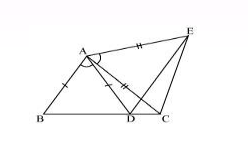
\includegraphics[width=\columnwidth]{figs/ABCDE.png}
	\caption{$\triangle ABC \hspace{12pt} and \hspace{12pt} \triangle ADE $}
 \label{fig:fig1}
\end{figure}
\textbf{Construction steps:}
		\begin{enumerate}[label=(\roman*)]
\item Let assume, the input parameters are, 
\begin{table}[H]
\centering
	\input{tables/table_1_bargav.tex}
	  \caption{Input Parameters}
	  \label{Table-1: }
\end{table}
$\therefore$ the output can be calculated as,
\begin{table}[H]
\centering
	\input{tables/table_2_bargav.tex}
	  \caption{Output Parameters}
	  \label{Table-2: }
\end{table}
$\therefore$ By, joining these points the required figure will be formed.
\begin{figure}[H]
    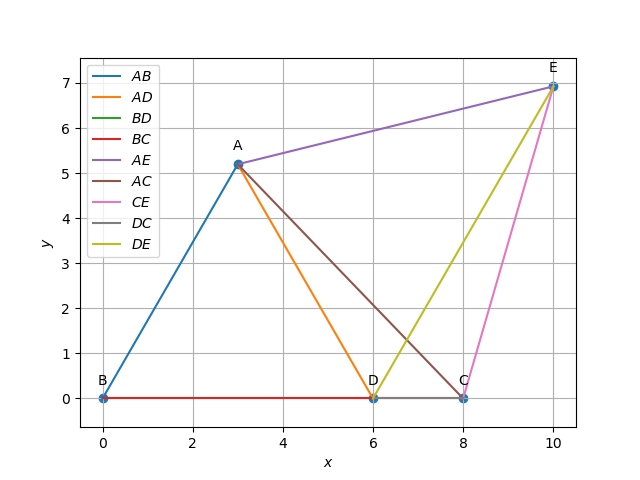
\includegraphics[width=\columnwidth]{figs/Final_python.png}
	\caption{$\triangle ABC \hspace{12pt} and \hspace{12pt} \triangle ADE$}
    \label{fig:fig2}
\end{figure}
\end{enumerate}
\end{enumerate}

\item 
	$AB$ is a line segment and $\vec{P}$ is its mid-point. $\vec{D}$ and $\vec{E}$ are points on the same side of
$AB$ such that $\angle BAD = \angle ABE$ and $\angle EPA = \angle DPB$. Show that
\label{chapters/9/7/1/7}
\begin{enumerate}
\item $\triangle DAP \cong \triangle EBP$
\item $AD = BE$.
\end{enumerate}
\solution
\begin{enumerate}[label=\thesection.\arabic*,ref=\thesection.\theenumi]
\numberwithin{equation}{enumi}
\numberwithin{figure}{enumi}
\numberwithin{table}{enumi}
\item Construct a triangle $ABC$ in which $BC=7cm, \angle{B}=75\degree$ and $AB + AC = 13 cm$.
\label{chapters/9/11/2/1}
%\input{chapters/9/11/2/1/line.tex}
%
\item Construct a triangle $ABC$ in which $BC=8cm, \angle{B}=45\degree$ and $AB - AC = 3.5 cm$.
\label{chapters/9/11/2/2}
\\
\solution
\input{chapters/9/11/2/2-new/vector-2.tex}
%
\item Construct a triangle $PQR$ in which $QR=6cm, \angle{Q}=60\degree$ and $PR - PQ = 2cm$.
\label{chapters/9/11/2/3}
%\input{chapters/9/11/2/3/line.tex}
%
\item Construct a triangle $XYZ$ in which $\angle{Y}=30\degree, \angle{Z}=90\degree$ and  $XY+YZ+ZX=11cm$.
\label{chapters/9/11/2/4}
%\input{chapters/9/11/2/4/line.tex}
%
\item Construct a right triangle whose base is 12cm and sum of its hypotenuse and other side is 18cm.
\label{chapters/9/11/2/5}
%\input{chapters/9/11/2/5/line.tex}
%
\item In Fig. \ref{fig:chapters/9/7/1/6/1}, $AC=AE,AB=AD$ and $\angle BAD=\angle EAC$. Show that $BC=DE$.
\label{chapters/9/7/1/6}
\begin{figure}[!h]
	\begin{center}
	\includegraphics[width=\columnwidth]{chapters/9/7/1/6/figs/fig.pdf}
	\end{center}
\caption{}
\label{fig:chapters/9/7/1/6/1}
\end{figure}
\\
\solution
\input{chapters/9/7/1/6/tri.tex}
\item 
	$AB$ is a line segment and $\vec{P}$ is its mid-point. $\vec{D}$ and $\vec{E}$ are points on the same side of
$AB$ such that $\angle BAD = \angle ABE$ and $\angle EPA = \angle DPB$. Show that
\label{chapters/9/7/1/7}
\begin{enumerate}
\item $\triangle DAP \cong \triangle EBP$
\item $AD = BE$.
\end{enumerate}
\solution
\input{chapters/9/7/1/7/tri.tex}
\item In right triangle ABC, right angled at C, M is the mid-point of hypotenuse AB. C is joined to M and produced to a point D such that DM = CM. Point D is joined to point B (see Figure \ref{fig:chapters/9/7/1/8/1}). Show that:
\begin{enumerate}
\item $\triangle AMC \cong \triangle BMD$
\item $\angle DBC$ is a right angle.
\item $\triangle DBC \cong \triangle ACB$
\item $CM = \dfrac{1}{2}AB$
\end{enumerate}
\label{chapters/9/7/1/8}
\input{chapters/9/7/1/8/vec.tex}
\item $AC = AE$ , $AB = AD$ and $\angle BAD = \angle EAC$. Show that $BC = DE$.
\begin{figure}[H]
    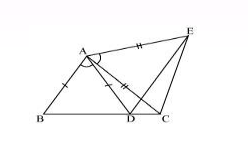
\includegraphics[width=\columnwidth]{figs/ABCDE.png}
	\caption{$\triangle ABC \hspace{12pt} and \hspace{12pt} \triangle ADE $}
 \label{fig:fig1}
\end{figure}
\textbf{Construction steps:}
		\begin{enumerate}[label=(\roman*)]
\item Let assume, the input parameters are, 
\begin{table}[H]
\centering
	\input{tables/table_1_bargav.tex}
	  \caption{Input Parameters}
	  \label{Table-1: }
\end{table}
$\therefore$ the output can be calculated as,
\begin{table}[H]
\centering
	\input{tables/table_2_bargav.tex}
	  \caption{Output Parameters}
	  \label{Table-2: }
\end{table}
$\therefore$ By, joining these points the required figure will be formed.
\begin{figure}[H]
    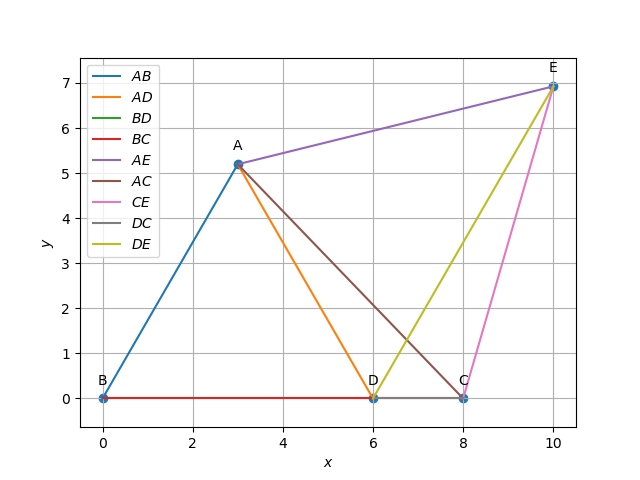
\includegraphics[width=\columnwidth]{figs/Final_python.png}
	\caption{$\triangle ABC \hspace{12pt} and \hspace{12pt} \triangle ADE$}
    \label{fig:fig2}
\end{figure}
\end{enumerate}
\end{enumerate}

\item In right triangle ABC, right angled at C, M is the mid-point of hypotenuse AB. C is joined to M and produced to a point D such that DM = CM. Point D is joined to point B (see Figure \ref{fig:chapters/9/7/1/8/1}). Show that:
\begin{enumerate}
\item $\triangle AMC \cong \triangle BMD$
\item $\angle DBC$ is a right angle.
\item $\triangle DBC \cong \triangle ACB$
\item $CM = \dfrac{1}{2}AB$
\end{enumerate}
\label{chapters/9/7/1/8}
\iffalse
\documentclass[10pt]{article}
\usepackage{graphicx}
\def\inputGnumericTable{}
\usepackage[latin1]{inputenc}
\usepackage{fullpage}
\usepackage{color}
\usepackage{array}
\usepackage{longtable}
\usepackage{calc}
\usepackage{multirow}
\usepackage{hhline}
\usepackage{ifthen}
\usepackage{amsmath}
\usepackage[none]{hyphenat}
\usepackage{listings}
\usepackage[english]{babel}
\usepackage{siunitx}
\usepackage{caption}
\usepackage{booktabs}
\usepackage{array}
\usepackage{extarrows}
\usepackage{enumerate}
\usepackage{enumitem}
\usepackage{amsmath}
\usepackage{commath}
\usepackage{gensymb}
\usepackage{amssymb}
\usepackage{multicol}
%\usepackage[utf8]{inputenc}
\lstset{
 frame=single,
 breaklines=true
}
\usepackage{hyperref}
\usepackage[margin=0.65in]{geometry}	 
%\usepackage{exsheets}% also loads the `tasks' package
\usepackage{atbegshi}
\AtBeginDocument{\AtBeginShipoutNext{\AtBeginShipoutDiscard}}

%new macro definitions
\renewcommand{\labelenumi}{(\roman{enumi})}
\newcommand{\mydet}[1]{\ensuremath{\begin{vmatrix}#1\end{vmatrix}}}
\providecommand{\brak}[1]{\ensuremath{\left(#1\right)}}
\newcommand{\solution}{\noindent \textbf{Solution: }}
\newcommand{\myvec}[1]{\ensuremath{\begin{pmatrix}#1\end{pmatrix}}}
\newenvironment{amatrix}[1]{%
	\left(\begin{array}{@{}*{#1}{c}|c@{}}
}{%
	\end{array}\right)
}

\newcommand{\myaugvec}[2]{\ensuremath{\begin{amatrix}{#1}#2\end{amatrix}}}
\providecommand{\norm}[1]{\left\1Vert#1\right\rVert}
\let\vec\mathbf{}


%\SetEnumitemKey{twocol}{
% before=\raggedcolumns\begin{multicols}{2},
% after=\end{multicols}}
%\SetEnumitemKey{fourcol}{
% before=\raggedcolumns\begin{multicols}{4},
% after=\end{multicols}} 


\begin{document}
\begin{center}
\title{\textbf{TRIANGLES}}
\date{\vspace{-5ex}}
\maketitle
\end{center}
\section*{9$^{th}$Math - Chapter 7}
This is Problem-8 from Exercise 7.1\\\\


\section*{\large Construction:}
\fi
The input parameters for construction
	are available in Table \ref{tab:chapters/9/7/1/8/table}.
\begin{table}[h!]
	\centering
	%\subimport{../chapters/9/7/1/8/tables/}{table.tex}
     \input{chapters/9/7/1/8/tables/table.tex}
	\caption{}
	\label{tab:chapters/9/7/1/8/table}
\end{table}
Thus, 
\begin{align}
	\vec{A}=\myvec{0\\b},\,
	\vec{B}=\myvec{a\\0},\,
	\vec{C}=\myvec{0\\0}
\end{align}
yielding
\begin{align}
	\vec{M}&=\frac{\vec{A}+\vec{B}}{2}=\frac{1}{2}\myvec{a\\b}
\end{align}
Also, 
\begin{align}
	\vec{M}&=\frac{\vec{C}+\vec{D}}{2}\\
	\implies \vec{D}&=2\vec{M}-\vec{C}=\myvec{a\\b}
\end{align}
\iffalse
\solution
Given
\begin{align}
	\vec{M}&=\frac{\vec{A}+\vec{B}}{2}
	\label{eq:chapters/9/7/1/8/1}\\
	\vec{D}-\vec{M}&=\vec{C}-\vec{M}
	\label{eq:chapters/9/7/1/8/2}\\
	\angle ACB&=90\degree
\end{align}
\textbf{Proof:} From Figure \ref{fig:chapters/9/7/1/8/1}
\fi
Thus,
\begin{align}
	\brak{\vec{D}-\vec{B}}^{\top}\brak{\vec{B}-\vec{C}} &= \myvec{0 & b}\myvec{a\\0}=0\\
	\implies BD & \perp BC\\
\end{align}
Also, 
\begin{align}
	\norm{\vec{A}-\vec{B}}&=\norm{\myvec{-a\\b}}\\
	\norm{\vec{C}-\vec{D}}&=\norm{\myvec{-a\\-b}}\\
	\implies \norm{\vec{A}-\vec{B}} &= \norm{\vec{C}-\vec{D}}\\
	\text{ or, } AB &= CD
	\label{eq:chapters/9/7/1/8/3}	
\end{align}
From \eqref{eq:chapters/9/7/1/8/3}
\begin{align}
	\implies CM = \frac{1}{2}CD = \frac{1}{2}AB 
\end{align}
See Fig. 
\ref{fig:chapters/9/7/1/8/1}.
\begin{figure}[H]
	\begin{center}
		\includegraphics[width=\columnwidth]{./chapters/9/7/1/8/figs/fig.pdf}
	\end{center}
\caption{}
\label{fig:chapters/9/7/1/8/1}
\end{figure}


\item $AC = AE$ , $AB = AD$ and $\angle BAD = \angle EAC$. Show that $BC = DE$.
\begin{figure}[H]
    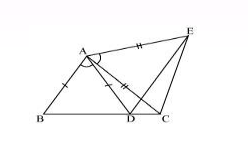
\includegraphics[width=\columnwidth]{figs/ABCDE.png}
	\caption{$\triangle ABC \hspace{12pt} and \hspace{12pt} \triangle ADE $}
 \label{fig:fig1}
\end{figure}
\textbf{Construction steps:}
		\begin{enumerate}[label=(\roman*)]
\item Let assume, the input parameters are, 
\begin{table}[H]
\centering
	\begin{tabular}{|c|c|p{5cm}|}
\hline
\textbf{Parameter} & \textbf{Value} & \textbf{Description} \\
\hline
	$\theta$ & $60\degree$ & $\angle{BAD} = \angle{CAE}$ \\
\hline
	$\vec{B}$ & $\myvec{0\\0}$ & Reference point at origin \\
\hline
	$\vec{D}$ & $\myvec{6\\0}$ & point $\vec{D}$ on the same axis of $\vec{B}$ \\
\hline
	$\vec{C}$ & $\myvec{8\\0}$ & point $\vec{C}$ on the same axis of $\vec{B}$ \\
\hline
\end{tabular}

	  \caption{Input Parameters}
	  \label{Table-1: }
\end{table}
$\therefore$ the output can be calculated as,
\begin{table}[H]
\centering
	\begin{tabular}{|c|c|p{5cm}|}
\hline
\textbf{Parameter} & \textbf{Value} & \textbf{Description} \\
\hline
	$BD$ & $\norm{\vec{B-D}}$ & Length of $BD$ \\
\hline
	$CD$ & $\norm{\vec{C-D}}$ & Length of $CD$ \\
\hline
	$\alpha$ & $\brak{\frac{180 - \theta}{2}}$ & $\angle ABD$ \\
\hline
	$AB$ & $BD \brak{\frac{\sin \alpha}{\sin \theta}}$ &  Length of $AB$ \\
\hline
	$\vec{A}$ & $\vec{B}$ + $\myvec{AB \cos \alpha  \\ AB \sin \alpha}$ & point $\vec{B}$ makes an angle $\alpha$  with line $(AB ,BD)$  \\
\hline
	$AD$ & $\norm{\vec{A-D}}$ & Length of $AD$ \\
\hline
	$AC$ & $\norm{\vec{A-C}}$ & Length of $AC$ \\
\hline
	  
	$\beta_1$ & $\cos^{-1} \brak{\frac{AC^2 +CD^2 - AD^2}{2 AC CD}}$ & $\angle ACD$ \\
\hline
	$CE$ & ${AC} \brak{\frac{\sin \theta}{\sin \alpha}}$ &  Length of $CE$ \\
\hline
	$\beta$ & $\alpha + \beta_1$ & $\angle ECB$\\

\hline
	$\vec{E}$ & $\vec{C}$ + $\myvec{-CE \cos \beta  \\ CE \sin \beta}$ & point $\vec{C}$ makes an angle $\beta$  with line $(BC ,CE)$  \\
\hline

\end{tabular}

	  \caption{Output Parameters}
	  \label{Table-2: }
\end{table}
$\therefore$ By, joining these points the required figure will be formed.
\begin{figure}[H]
    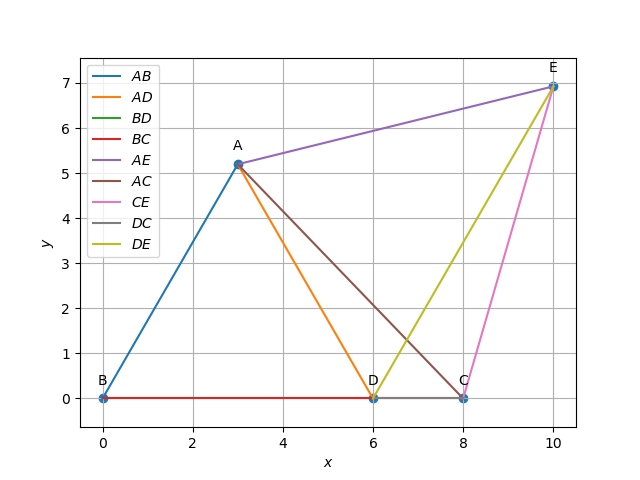
\includegraphics[width=\columnwidth]{figs/Final_python.png}
	\caption{$\triangle ABC \hspace{12pt} and \hspace{12pt} \triangle ADE$}
    \label{fig:fig2}
\end{figure}
\end{enumerate}
\end{enumerate}

\item 
	$AB$ is a line segment and $\vec{P}$ is its mid-point. $\vec{D}$ and $\vec{E}$ are points on the same side of
$AB$ such that $\angle BAD = \angle ABE$ and $\angle EPA = \angle DPB$. Show that
\label{chapters/9/7/1/7}
\begin{enumerate}
\item $\triangle DAP \cong \triangle EBP$
\item $AD = BE$.
\end{enumerate}
\solution
\begin{enumerate}[label=\thesection.\arabic*,ref=\thesection.\theenumi]
\numberwithin{equation}{enumi}
\numberwithin{figure}{enumi}
\numberwithin{table}{enumi}
\item Construct a triangle $ABC$ in which $BC=7cm, \angle{B}=75\degree$ and $AB + AC = 13 cm$.
\label{chapters/9/11/2/1}
%%\documentclass[12pt]{article}
%\usepackage[cmex10]{amsmath}
%\usepackage{amsthm}
%\usepackage{mathrsfs}
%\usepackage{txfonts}
%\usepackage{stfloats}
%\usepackage{bm}
%\usepackage{cite}
%\usepackage{cases}
%\usepackage{subfig}
%\usepackage{longtable}
%\usepackage{multirow}
%\usepackage{enumitem}
%\usepackage{mathtools}
%\usepackage{steinmetz}
%\usepackage{tikz}
%\usepackage{circuitikz}
%\usepackage{verbatim}
%\usepackage{tfrupee}
%\usepackage[breaklinks=true]{hyperref}
%\usepackage{tkz-euclide} % loads  TikZ and tkz-base
%\providecommand{\brak}[1]{\ensuremath{\left(#1\right)}}
%\usepackage{atbegshi}
%\AtBeginDocument{\AtBeginShipoutNext{\AtBeginShipoutDiscard}}
%\usetikzlibrary{calc,math}
%\usepackage{listings}
%    \usepackage{color}                                            %%
%    \usepackage{array}                                            %%
 %   \usepackage{longtable}                                        %%
  %  \usepackage{calc}                                             %%
   % \usepackage{multirow}                                         %%
    %\usepackage{hhline}                                           %%
    %\usepackage{ifthen}                                           %%
  %optionally (for landscape tables embedded in another document): %%
    %\usepackage{lscape}     
%\usepackage{multicol}
%\usepackage{chngcntr}

%\DeclareMathOperator*{\Res}{Res}
%\renewcommand{\baselinestretch}{2}
%\renewcommand\thesection{\arabic{section}}
%\renewcommand\thesubsection{\thesection.\arabic{subsection}}
%\renewcommand\thesubsubsection{\thesubsection.\arabic{subsubsection}}


% correct bad hyphenation here
%\hyphenation{op-tical net-works semi-conduc-tor}
%\def\inputGnumericTable{}                                 %%

%\lstset{
%language=C,
%frame=single, 
%breaklines=true,
%columns=fullflexible
%}
%\begin{document}
%\newtheorem{theorem}{Theorem}[section]
%\newtheorem{problem}{Problem}
%\newtheorem{proposition}{Proposition}[section]
%\newtheorem{lemma}{Lemma}[section]
%\newtheorem{corollary}[theorem]{Corollary}
%\newtheorem{example}{Example}[section]
%\newtheorem{definition}[problem]{Definition}
%\newcommand{\BEQA}{\begin{eqnarray}}
%\newcommand{\EEQA}{\end{eqnarray}}
%\newcommand{\define}{\stackrel{\triangle}{=}}

%\bibliographystyle{IEEEtran}
%\bibliographystyle{ieeetr}
%\providecommand{\mbf}{\mathbf}
%\providecommand{\pr}[1]{\ensuremath{\Pr\left(#1\right)}}
%\providecommand{\qfunc}[1]{\ensuremath{Q\left(#1\right)}}
%\providecommand{\sbrak}[1]{\ensuremath{{}\left[#1\right]}}
%\providecommand{\lsbrak}[1]{\ensuremath{{}\left[#1\right.}}
%\providecommand{\rsbrak}[1]{\ensuremath{{}\left.#1\right]}}
%\providecommand{\brak}[1]{\ensuremath{\left(#1\right)}}
%\providecommand{\lbrak}[1]{\ensuremath{\left(#1\right.}}
%\providecommand{\rbrak}[1]{\ensuremath{\left.#1\right)}}
%\providecommand{\cbrak}[1]{\ensuremath{\left\{#1\right\}}}
%\providecommand{\lcbrak}[1]{\ensuremath{\left\{#1\right.}}
%\providecommand{\rcbrak}[1]{\ensuremath{\left.#1\right\}}}
%\theoremstyle{remark}
%\newtheorem{rem}{Remark}
%\newcommand{\sgn}{\mathop{\mathrm{sgn}}}
%\providecommand{\res}[1]{\Res\displaylimits_{#1}} 
%\providecommand{\mtx}[1]{\mathbf{#1}}
%\providecommand{\fourier}{\overset{\mathcal{F}}{\rightleftharpoons}}
%\providecommand{\system}{\overset{\mathcal{H}}{\longleftrightarrow}}
	%\newcommand{\solution}[2]{\textbf{Solution:}{#1}}
%\newcommand{\solution}{\noindent \textbf{Solution: }}
%\newcommand{\cosec}{\,\text{cosec}\,}
%\providecommand{\dec}[2]{\ensuremath{\overset{#1}{\underset{#2}{\gtrless}}}}
%\newcommand{\myvec}[1]{\ensuremath{\begin{pmatrix}#1\end{pmatrix}}}
%\newcommand{\mydet}[1]{\ensuremath{\begin{vmatrix}#1\end{vmatrix}}}
%\let\vec\mathbf
%\begin{center}
%\title{\textbf{Straight Lines}}
%\date{\vspace{-5ex}} %Not to print date automatically
%\maketitle
%\end{center}
%\setcounter{page}{1}
%\section*{11$^{th}$ Maths - Chapter 10}
%This is Problem-10 from Exercise 10.4
%\begin{enumerate}
%    \item If three lines whose equations are $y=m_1x+c_1$, $y=m_2x+c_2$ and $y=m_3x+c_3$ are concurrent, then show that $m_1(c_2-c_3)+m_2(c_3-c_1)+m_3(c_1-c_2) = 0.$\\
%    \solution 
    Given lines can be written as \begin{align}
       m_1x-y+c_1=0
    \end{align}
    \begin{align}
        m_2x-y+c_2=0
    \end{align}
    \begin{align}
        m_3x-y+c_3=0
        \label{eq:3}
    \end{align}
    
    
   The above lines can be written in the form of \begin{align}
        \Vec{n}^{\top}\Vec{x} = c
    \end{align}
   Therefore,
		\begin{align}
       \myvec{m_1&-1}\vec{x}=c_1
       \label{eq:5}
   \end{align} 
   \begin{align}
       \myvec{m_2&-1}\vec{x}=c_2
       \label{eq:6}
   \end{align}
   \begin{align}
       \myvec{m_3&-1}\vec{x}=c_3
       \label{eq:7}
   \end{align}
   Solving equations \eqref{eq:5}, \eqref{eq:6}and \eqref{eq:7}
		augumented matrix is
 \begin{align}
    \myvec{m_1&-1&c_1\\m_2&-1&c_2\\m_3&-1&c_3}\\
    \xleftrightarrow{R_2 \leftarrow m_1R_2-m_2R_1}
    \myvec{m_1&-1&c_1\\0&m_2-m_1&m_1c_2-m_2c_1\\m_3&-1&c_3}\\
    \xleftrightarrow{R_3 \leftarrow m_1R_3-m_3R_1}
    \myvec{m_1&-1&c_1\\0&m_2-m_1&m_1c_2-m_2c_1\\0&m_3-m_1&m_1c_3-m_3c_1}\\
    \xleftrightarrow{R_3 \leftarrow R_3\frac{m_2-m_1}{m_3-m_1}-R_2}
        \myvec{m_1&-1&c_1\\0&m_2-m_1&m_1c_2-m_2c_1\\0&0&$\brak{m_1c_3-m_3c_1}$$\brak{\frac{m_2-m_1}{m_3-m_1}}$-$\brak{m_1c_2-m_2c_1}$}
\end{align}
Now, for lines to be concurrent, then the third row should be equal to zero. \\

Therefore,
\begin{align}
\brak{m_1c_3-m_3c_1}\brak{\frac{m_2-m_1}{m_3-m_1}}-\brak{m_1c_2-m_2c_1}=0\\
\frac{\brak{m_1c_3-m_3c_1}\brak{m_2-m_1}-\brak{m_1c_2-m_2c_1}\brak{m_3-m_1}}{m_3-m_1}=0\\
\brak{m_1c_3-m_3c_1}\brak{m_2-m_1}-\brak{m_1c_2-m_2c_1}\brak{m_3-m_1}=0\\
m_2c_3-m_1c_3+m_3c_1-m_3c_2+m_1c_2-m_2c_1=0\\
m_1\brak{c_2-c_3}+m_2\brak{c_3-c_1}+m_3\brak{c_1-c_2} = 0
\end{align}
           Hence proved
%\begin{figure}[h]
 %   \centering
  %  \includegraphics[width=\columnwidth]{concurrent-1.png}
   % \caption{Straight Lines}
    %\label{fig:concurrent-1.png}
%\end{figure}
%\end{enumerate}
%\end{document}

%
\item Construct a triangle $ABC$ in which $BC=8cm, \angle{B}=45\degree$ and $AB - AC = 3.5 cm$.
\label{chapters/9/11/2/2}
\\
\solution
\input{chapters/9/11/2/2-new/vector-2.tex}
%
\item Construct a triangle $PQR$ in which $QR=6cm, \angle{Q}=60\degree$ and $PR - PQ = 2cm$.
\label{chapters/9/11/2/3}
%%\documentclass[12pt]{article}
%\usepackage[cmex10]{amsmath}
%\usepackage{amsthm}
%\usepackage{mathrsfs}
%\usepackage{txfonts}
%\usepackage{stfloats}
%\usepackage{bm}
%\usepackage{cite}
%\usepackage{cases}
%\usepackage{subfig}
%\usepackage{longtable}
%\usepackage{multirow}
%\usepackage{enumitem}
%\usepackage{mathtools}
%\usepackage{steinmetz}
%\usepackage{tikz}
%\usepackage{circuitikz}
%\usepackage{verbatim}
%\usepackage{tfrupee}
%\usepackage[breaklinks=true]{hyperref}
%\usepackage{tkz-euclide} % loads  TikZ and tkz-base
%\providecommand{\brak}[1]{\ensuremath{\left(#1\right)}}
%\usepackage{atbegshi}
%\AtBeginDocument{\AtBeginShipoutNext{\AtBeginShipoutDiscard}}
%\usetikzlibrary{calc,math}
%\usepackage{listings}
%    \usepackage{color}                                            %%
%    \usepackage{array}                                            %%
 %   \usepackage{longtable}                                        %%
  %  \usepackage{calc}                                             %%
   % \usepackage{multirow}                                         %%
    %\usepackage{hhline}                                           %%
    %\usepackage{ifthen}                                           %%
  %optionally (for landscape tables embedded in another document): %%
    %\usepackage{lscape}     
%\usepackage{multicol}
%\usepackage{chngcntr}

%\DeclareMathOperator*{\Res}{Res}
%\renewcommand{\baselinestretch}{2}
%\renewcommand\thesection{\arabic{section}}
%\renewcommand\thesubsection{\thesection.\arabic{subsection}}
%\renewcommand\thesubsubsection{\thesubsection.\arabic{subsubsection}}


% correct bad hyphenation here
%\hyphenation{op-tical net-works semi-conduc-tor}
%\def\inputGnumericTable{}                                 %%

%\lstset{
%language=C,
%frame=single, 
%breaklines=true,
%columns=fullflexible
%}
%\begin{document}
%\newtheorem{theorem}{Theorem}[section]
%\newtheorem{problem}{Problem}
%\newtheorem{proposition}{Proposition}[section]
%\newtheorem{lemma}{Lemma}[section]
%\newtheorem{corollary}[theorem]{Corollary}
%\newtheorem{example}{Example}[section]
%\newtheorem{definition}[problem]{Definition}
%\newcommand{\BEQA}{\begin{eqnarray}}
%\newcommand{\EEQA}{\end{eqnarray}}
%\newcommand{\define}{\stackrel{\triangle}{=}}

%\bibliographystyle{IEEEtran}
%\bibliographystyle{ieeetr}
%\providecommand{\mbf}{\mathbf}
%\providecommand{\pr}[1]{\ensuremath{\Pr\left(#1\right)}}
%\providecommand{\qfunc}[1]{\ensuremath{Q\left(#1\right)}}
%\providecommand{\sbrak}[1]{\ensuremath{{}\left[#1\right]}}
%\providecommand{\lsbrak}[1]{\ensuremath{{}\left[#1\right.}}
%\providecommand{\rsbrak}[1]{\ensuremath{{}\left.#1\right]}}
%\providecommand{\brak}[1]{\ensuremath{\left(#1\right)}}
%\providecommand{\lbrak}[1]{\ensuremath{\left(#1\right.}}
%\providecommand{\rbrak}[1]{\ensuremath{\left.#1\right)}}
%\providecommand{\cbrak}[1]{\ensuremath{\left\{#1\right\}}}
%\providecommand{\lcbrak}[1]{\ensuremath{\left\{#1\right.}}
%\providecommand{\rcbrak}[1]{\ensuremath{\left.#1\right\}}}
%\theoremstyle{remark}
%\newtheorem{rem}{Remark}
%\newcommand{\sgn}{\mathop{\mathrm{sgn}}}
%\providecommand{\res}[1]{\Res\displaylimits_{#1}} 
%\providecommand{\mtx}[1]{\mathbf{#1}}
%\providecommand{\fourier}{\overset{\mathcal{F}}{\rightleftharpoons}}
%\providecommand{\system}{\overset{\mathcal{H}}{\longleftrightarrow}}
	%\newcommand{\solution}[2]{\textbf{Solution:}{#1}}
%\newcommand{\solution}{\noindent \textbf{Solution: }}
%\newcommand{\cosec}{\,\text{cosec}\,}
%\providecommand{\dec}[2]{\ensuremath{\overset{#1}{\underset{#2}{\gtrless}}}}
%\newcommand{\myvec}[1]{\ensuremath{\begin{pmatrix}#1\end{pmatrix}}}
%\newcommand{\mydet}[1]{\ensuremath{\begin{vmatrix}#1\end{vmatrix}}}
%\let\vec\mathbf
%\begin{center}
%\title{\textbf{Straight Lines}}
%\date{\vspace{-5ex}} %Not to print date automatically
%\maketitle
%\end{center}
%\setcounter{page}{1}
%\section*{11$^{th}$ Maths - Chapter 10}
%This is Problem-10 from Exercise 10.4
%\begin{enumerate}
%    \item If three lines whose equations are $y=m_1x+c_1$, $y=m_2x+c_2$ and $y=m_3x+c_3$ are concurrent, then show that $m_1(c_2-c_3)+m_2(c_3-c_1)+m_3(c_1-c_2) = 0.$\\
%    \solution 
    Given lines can be written as \begin{align}
       m_1x-y+c_1=0
    \end{align}
    \begin{align}
        m_2x-y+c_2=0
    \end{align}
    \begin{align}
        m_3x-y+c_3=0
        \label{eq:3}
    \end{align}
    
    
   The above lines can be written in the form of \begin{align}
        \Vec{n}^{\top}\Vec{x} = c
    \end{align}
   Therefore,
		\begin{align}
       \myvec{m_1&-1}\vec{x}=c_1
       \label{eq:5}
   \end{align} 
   \begin{align}
       \myvec{m_2&-1}\vec{x}=c_2
       \label{eq:6}
   \end{align}
   \begin{align}
       \myvec{m_3&-1}\vec{x}=c_3
       \label{eq:7}
   \end{align}
   Solving equations \eqref{eq:5}, \eqref{eq:6}and \eqref{eq:7}
		augumented matrix is
 \begin{align}
    \myvec{m_1&-1&c_1\\m_2&-1&c_2\\m_3&-1&c_3}\\
    \xleftrightarrow{R_2 \leftarrow m_1R_2-m_2R_1}
    \myvec{m_1&-1&c_1\\0&m_2-m_1&m_1c_2-m_2c_1\\m_3&-1&c_3}\\
    \xleftrightarrow{R_3 \leftarrow m_1R_3-m_3R_1}
    \myvec{m_1&-1&c_1\\0&m_2-m_1&m_1c_2-m_2c_1\\0&m_3-m_1&m_1c_3-m_3c_1}\\
    \xleftrightarrow{R_3 \leftarrow R_3\frac{m_2-m_1}{m_3-m_1}-R_2}
        \myvec{m_1&-1&c_1\\0&m_2-m_1&m_1c_2-m_2c_1\\0&0&$\brak{m_1c_3-m_3c_1}$$\brak{\frac{m_2-m_1}{m_3-m_1}}$-$\brak{m_1c_2-m_2c_1}$}
\end{align}
Now, for lines to be concurrent, then the third row should be equal to zero. \\

Therefore,
\begin{align}
\brak{m_1c_3-m_3c_1}\brak{\frac{m_2-m_1}{m_3-m_1}}-\brak{m_1c_2-m_2c_1}=0\\
\frac{\brak{m_1c_3-m_3c_1}\brak{m_2-m_1}-\brak{m_1c_2-m_2c_1}\brak{m_3-m_1}}{m_3-m_1}=0\\
\brak{m_1c_3-m_3c_1}\brak{m_2-m_1}-\brak{m_1c_2-m_2c_1}\brak{m_3-m_1}=0\\
m_2c_3-m_1c_3+m_3c_1-m_3c_2+m_1c_2-m_2c_1=0\\
m_1\brak{c_2-c_3}+m_2\brak{c_3-c_1}+m_3\brak{c_1-c_2} = 0
\end{align}
           Hence proved
%\begin{figure}[h]
 %   \centering
  %  \includegraphics[width=\columnwidth]{concurrent-1.png}
   % \caption{Straight Lines}
    %\label{fig:concurrent-1.png}
%\end{figure}
%\end{enumerate}
%\end{document}

%
\item Construct a triangle $XYZ$ in which $\angle{Y}=30\degree, \angle{Z}=90\degree$ and  $XY+YZ+ZX=11cm$.
\label{chapters/9/11/2/4}
%%\documentclass[12pt]{article}
%\usepackage[cmex10]{amsmath}
%\usepackage{amsthm}
%\usepackage{mathrsfs}
%\usepackage{txfonts}
%\usepackage{stfloats}
%\usepackage{bm}
%\usepackage{cite}
%\usepackage{cases}
%\usepackage{subfig}
%\usepackage{longtable}
%\usepackage{multirow}
%\usepackage{enumitem}
%\usepackage{mathtools}
%\usepackage{steinmetz}
%\usepackage{tikz}
%\usepackage{circuitikz}
%\usepackage{verbatim}
%\usepackage{tfrupee}
%\usepackage[breaklinks=true]{hyperref}
%\usepackage{tkz-euclide} % loads  TikZ and tkz-base
%\providecommand{\brak}[1]{\ensuremath{\left(#1\right)}}
%\usepackage{atbegshi}
%\AtBeginDocument{\AtBeginShipoutNext{\AtBeginShipoutDiscard}}
%\usetikzlibrary{calc,math}
%\usepackage{listings}
%    \usepackage{color}                                            %%
%    \usepackage{array}                                            %%
 %   \usepackage{longtable}                                        %%
  %  \usepackage{calc}                                             %%
   % \usepackage{multirow}                                         %%
    %\usepackage{hhline}                                           %%
    %\usepackage{ifthen}                                           %%
  %optionally (for landscape tables embedded in another document): %%
    %\usepackage{lscape}     
%\usepackage{multicol}
%\usepackage{chngcntr}

%\DeclareMathOperator*{\Res}{Res}
%\renewcommand{\baselinestretch}{2}
%\renewcommand\thesection{\arabic{section}}
%\renewcommand\thesubsection{\thesection.\arabic{subsection}}
%\renewcommand\thesubsubsection{\thesubsection.\arabic{subsubsection}}


% correct bad hyphenation here
%\hyphenation{op-tical net-works semi-conduc-tor}
%\def\inputGnumericTable{}                                 %%

%\lstset{
%language=C,
%frame=single, 
%breaklines=true,
%columns=fullflexible
%}
%\begin{document}
%\newtheorem{theorem}{Theorem}[section]
%\newtheorem{problem}{Problem}
%\newtheorem{proposition}{Proposition}[section]
%\newtheorem{lemma}{Lemma}[section]
%\newtheorem{corollary}[theorem]{Corollary}
%\newtheorem{example}{Example}[section]
%\newtheorem{definition}[problem]{Definition}
%\newcommand{\BEQA}{\begin{eqnarray}}
%\newcommand{\EEQA}{\end{eqnarray}}
%\newcommand{\define}{\stackrel{\triangle}{=}}

%\bibliographystyle{IEEEtran}
%\bibliographystyle{ieeetr}
%\providecommand{\mbf}{\mathbf}
%\providecommand{\pr}[1]{\ensuremath{\Pr\left(#1\right)}}
%\providecommand{\qfunc}[1]{\ensuremath{Q\left(#1\right)}}
%\providecommand{\sbrak}[1]{\ensuremath{{}\left[#1\right]}}
%\providecommand{\lsbrak}[1]{\ensuremath{{}\left[#1\right.}}
%\providecommand{\rsbrak}[1]{\ensuremath{{}\left.#1\right]}}
%\providecommand{\brak}[1]{\ensuremath{\left(#1\right)}}
%\providecommand{\lbrak}[1]{\ensuremath{\left(#1\right.}}
%\providecommand{\rbrak}[1]{\ensuremath{\left.#1\right)}}
%\providecommand{\cbrak}[1]{\ensuremath{\left\{#1\right\}}}
%\providecommand{\lcbrak}[1]{\ensuremath{\left\{#1\right.}}
%\providecommand{\rcbrak}[1]{\ensuremath{\left.#1\right\}}}
%\theoremstyle{remark}
%\newtheorem{rem}{Remark}
%\newcommand{\sgn}{\mathop{\mathrm{sgn}}}
%\providecommand{\res}[1]{\Res\displaylimits_{#1}} 
%\providecommand{\mtx}[1]{\mathbf{#1}}
%\providecommand{\fourier}{\overset{\mathcal{F}}{\rightleftharpoons}}
%\providecommand{\system}{\overset{\mathcal{H}}{\longleftrightarrow}}
	%\newcommand{\solution}[2]{\textbf{Solution:}{#1}}
%\newcommand{\solution}{\noindent \textbf{Solution: }}
%\newcommand{\cosec}{\,\text{cosec}\,}
%\providecommand{\dec}[2]{\ensuremath{\overset{#1}{\underset{#2}{\gtrless}}}}
%\newcommand{\myvec}[1]{\ensuremath{\begin{pmatrix}#1\end{pmatrix}}}
%\newcommand{\mydet}[1]{\ensuremath{\begin{vmatrix}#1\end{vmatrix}}}
%\let\vec\mathbf
%\begin{center}
%\title{\textbf{Straight Lines}}
%\date{\vspace{-5ex}} %Not to print date automatically
%\maketitle
%\end{center}
%\setcounter{page}{1}
%\section*{11$^{th}$ Maths - Chapter 10}
%This is Problem-10 from Exercise 10.4
%\begin{enumerate}
%    \item If three lines whose equations are $y=m_1x+c_1$, $y=m_2x+c_2$ and $y=m_3x+c_3$ are concurrent, then show that $m_1(c_2-c_3)+m_2(c_3-c_1)+m_3(c_1-c_2) = 0.$\\
%    \solution 
    Given lines can be written as \begin{align}
       m_1x-y+c_1=0
    \end{align}
    \begin{align}
        m_2x-y+c_2=0
    \end{align}
    \begin{align}
        m_3x-y+c_3=0
        \label{eq:3}
    \end{align}
    
    
   The above lines can be written in the form of \begin{align}
        \Vec{n}^{\top}\Vec{x} = c
    \end{align}
   Therefore,
		\begin{align}
       \myvec{m_1&-1}\vec{x}=c_1
       \label{eq:5}
   \end{align} 
   \begin{align}
       \myvec{m_2&-1}\vec{x}=c_2
       \label{eq:6}
   \end{align}
   \begin{align}
       \myvec{m_3&-1}\vec{x}=c_3
       \label{eq:7}
   \end{align}
   Solving equations \eqref{eq:5}, \eqref{eq:6}and \eqref{eq:7}
		augumented matrix is
 \begin{align}
    \myvec{m_1&-1&c_1\\m_2&-1&c_2\\m_3&-1&c_3}\\
    \xleftrightarrow{R_2 \leftarrow m_1R_2-m_2R_1}
    \myvec{m_1&-1&c_1\\0&m_2-m_1&m_1c_2-m_2c_1\\m_3&-1&c_3}\\
    \xleftrightarrow{R_3 \leftarrow m_1R_3-m_3R_1}
    \myvec{m_1&-1&c_1\\0&m_2-m_1&m_1c_2-m_2c_1\\0&m_3-m_1&m_1c_3-m_3c_1}\\
    \xleftrightarrow{R_3 \leftarrow R_3\frac{m_2-m_1}{m_3-m_1}-R_2}
        \myvec{m_1&-1&c_1\\0&m_2-m_1&m_1c_2-m_2c_1\\0&0&$\brak{m_1c_3-m_3c_1}$$\brak{\frac{m_2-m_1}{m_3-m_1}}$-$\brak{m_1c_2-m_2c_1}$}
\end{align}
Now, for lines to be concurrent, then the third row should be equal to zero. \\

Therefore,
\begin{align}
\brak{m_1c_3-m_3c_1}\brak{\frac{m_2-m_1}{m_3-m_1}}-\brak{m_1c_2-m_2c_1}=0\\
\frac{\brak{m_1c_3-m_3c_1}\brak{m_2-m_1}-\brak{m_1c_2-m_2c_1}\brak{m_3-m_1}}{m_3-m_1}=0\\
\brak{m_1c_3-m_3c_1}\brak{m_2-m_1}-\brak{m_1c_2-m_2c_1}\brak{m_3-m_1}=0\\
m_2c_3-m_1c_3+m_3c_1-m_3c_2+m_1c_2-m_2c_1=0\\
m_1\brak{c_2-c_3}+m_2\brak{c_3-c_1}+m_3\brak{c_1-c_2} = 0
\end{align}
           Hence proved
%\begin{figure}[h]
 %   \centering
  %  \includegraphics[width=\columnwidth]{concurrent-1.png}
   % \caption{Straight Lines}
    %\label{fig:concurrent-1.png}
%\end{figure}
%\end{enumerate}
%\end{document}

%
\item Construct a right triangle whose base is 12cm and sum of its hypotenuse and other side is 18cm.
\label{chapters/9/11/2/5}
%%\documentclass[12pt]{article}
%\usepackage[cmex10]{amsmath}
%\usepackage{amsthm}
%\usepackage{mathrsfs}
%\usepackage{txfonts}
%\usepackage{stfloats}
%\usepackage{bm}
%\usepackage{cite}
%\usepackage{cases}
%\usepackage{subfig}
%\usepackage{longtable}
%\usepackage{multirow}
%\usepackage{enumitem}
%\usepackage{mathtools}
%\usepackage{steinmetz}
%\usepackage{tikz}
%\usepackage{circuitikz}
%\usepackage{verbatim}
%\usepackage{tfrupee}
%\usepackage[breaklinks=true]{hyperref}
%\usepackage{tkz-euclide} % loads  TikZ and tkz-base
%\providecommand{\brak}[1]{\ensuremath{\left(#1\right)}}
%\usepackage{atbegshi}
%\AtBeginDocument{\AtBeginShipoutNext{\AtBeginShipoutDiscard}}
%\usetikzlibrary{calc,math}
%\usepackage{listings}
%    \usepackage{color}                                            %%
%    \usepackage{array}                                            %%
 %   \usepackage{longtable}                                        %%
  %  \usepackage{calc}                                             %%
   % \usepackage{multirow}                                         %%
    %\usepackage{hhline}                                           %%
    %\usepackage{ifthen}                                           %%
  %optionally (for landscape tables embedded in another document): %%
    %\usepackage{lscape}     
%\usepackage{multicol}
%\usepackage{chngcntr}

%\DeclareMathOperator*{\Res}{Res}
%\renewcommand{\baselinestretch}{2}
%\renewcommand\thesection{\arabic{section}}
%\renewcommand\thesubsection{\thesection.\arabic{subsection}}
%\renewcommand\thesubsubsection{\thesubsection.\arabic{subsubsection}}


% correct bad hyphenation here
%\hyphenation{op-tical net-works semi-conduc-tor}
%\def\inputGnumericTable{}                                 %%

%\lstset{
%language=C,
%frame=single, 
%breaklines=true,
%columns=fullflexible
%}
%\begin{document}
%\newtheorem{theorem}{Theorem}[section]
%\newtheorem{problem}{Problem}
%\newtheorem{proposition}{Proposition}[section]
%\newtheorem{lemma}{Lemma}[section]
%\newtheorem{corollary}[theorem]{Corollary}
%\newtheorem{example}{Example}[section]
%\newtheorem{definition}[problem]{Definition}
%\newcommand{\BEQA}{\begin{eqnarray}}
%\newcommand{\EEQA}{\end{eqnarray}}
%\newcommand{\define}{\stackrel{\triangle}{=}}

%\bibliographystyle{IEEEtran}
%\bibliographystyle{ieeetr}
%\providecommand{\mbf}{\mathbf}
%\providecommand{\pr}[1]{\ensuremath{\Pr\left(#1\right)}}
%\providecommand{\qfunc}[1]{\ensuremath{Q\left(#1\right)}}
%\providecommand{\sbrak}[1]{\ensuremath{{}\left[#1\right]}}
%\providecommand{\lsbrak}[1]{\ensuremath{{}\left[#1\right.}}
%\providecommand{\rsbrak}[1]{\ensuremath{{}\left.#1\right]}}
%\providecommand{\brak}[1]{\ensuremath{\left(#1\right)}}
%\providecommand{\lbrak}[1]{\ensuremath{\left(#1\right.}}
%\providecommand{\rbrak}[1]{\ensuremath{\left.#1\right)}}
%\providecommand{\cbrak}[1]{\ensuremath{\left\{#1\right\}}}
%\providecommand{\lcbrak}[1]{\ensuremath{\left\{#1\right.}}
%\providecommand{\rcbrak}[1]{\ensuremath{\left.#1\right\}}}
%\theoremstyle{remark}
%\newtheorem{rem}{Remark}
%\newcommand{\sgn}{\mathop{\mathrm{sgn}}}
%\providecommand{\res}[1]{\Res\displaylimits_{#1}} 
%\providecommand{\mtx}[1]{\mathbf{#1}}
%\providecommand{\fourier}{\overset{\mathcal{F}}{\rightleftharpoons}}
%\providecommand{\system}{\overset{\mathcal{H}}{\longleftrightarrow}}
	%\newcommand{\solution}[2]{\textbf{Solution:}{#1}}
%\newcommand{\solution}{\noindent \textbf{Solution: }}
%\newcommand{\cosec}{\,\text{cosec}\,}
%\providecommand{\dec}[2]{\ensuremath{\overset{#1}{\underset{#2}{\gtrless}}}}
%\newcommand{\myvec}[1]{\ensuremath{\begin{pmatrix}#1\end{pmatrix}}}
%\newcommand{\mydet}[1]{\ensuremath{\begin{vmatrix}#1\end{vmatrix}}}
%\let\vec\mathbf
%\begin{center}
%\title{\textbf{Straight Lines}}
%\date{\vspace{-5ex}} %Not to print date automatically
%\maketitle
%\end{center}
%\setcounter{page}{1}
%\section*{11$^{th}$ Maths - Chapter 10}
%This is Problem-10 from Exercise 10.4
%\begin{enumerate}
%    \item If three lines whose equations are $y=m_1x+c_1$, $y=m_2x+c_2$ and $y=m_3x+c_3$ are concurrent, then show that $m_1(c_2-c_3)+m_2(c_3-c_1)+m_3(c_1-c_2) = 0.$\\
%    \solution 
    Given lines can be written as \begin{align}
       m_1x-y+c_1=0
    \end{align}
    \begin{align}
        m_2x-y+c_2=0
    \end{align}
    \begin{align}
        m_3x-y+c_3=0
        \label{eq:3}
    \end{align}
    
    
   The above lines can be written in the form of \begin{align}
        \Vec{n}^{\top}\Vec{x} = c
    \end{align}
   Therefore,
		\begin{align}
       \myvec{m_1&-1}\vec{x}=c_1
       \label{eq:5}
   \end{align} 
   \begin{align}
       \myvec{m_2&-1}\vec{x}=c_2
       \label{eq:6}
   \end{align}
   \begin{align}
       \myvec{m_3&-1}\vec{x}=c_3
       \label{eq:7}
   \end{align}
   Solving equations \eqref{eq:5}, \eqref{eq:6}and \eqref{eq:7}
		augumented matrix is
 \begin{align}
    \myvec{m_1&-1&c_1\\m_2&-1&c_2\\m_3&-1&c_3}\\
    \xleftrightarrow{R_2 \leftarrow m_1R_2-m_2R_1}
    \myvec{m_1&-1&c_1\\0&m_2-m_1&m_1c_2-m_2c_1\\m_3&-1&c_3}\\
    \xleftrightarrow{R_3 \leftarrow m_1R_3-m_3R_1}
    \myvec{m_1&-1&c_1\\0&m_2-m_1&m_1c_2-m_2c_1\\0&m_3-m_1&m_1c_3-m_3c_1}\\
    \xleftrightarrow{R_3 \leftarrow R_3\frac{m_2-m_1}{m_3-m_1}-R_2}
        \myvec{m_1&-1&c_1\\0&m_2-m_1&m_1c_2-m_2c_1\\0&0&$\brak{m_1c_3-m_3c_1}$$\brak{\frac{m_2-m_1}{m_3-m_1}}$-$\brak{m_1c_2-m_2c_1}$}
\end{align}
Now, for lines to be concurrent, then the third row should be equal to zero. \\

Therefore,
\begin{align}
\brak{m_1c_3-m_3c_1}\brak{\frac{m_2-m_1}{m_3-m_1}}-\brak{m_1c_2-m_2c_1}=0\\
\frac{\brak{m_1c_3-m_3c_1}\brak{m_2-m_1}-\brak{m_1c_2-m_2c_1}\brak{m_3-m_1}}{m_3-m_1}=0\\
\brak{m_1c_3-m_3c_1}\brak{m_2-m_1}-\brak{m_1c_2-m_2c_1}\brak{m_3-m_1}=0\\
m_2c_3-m_1c_3+m_3c_1-m_3c_2+m_1c_2-m_2c_1=0\\
m_1\brak{c_2-c_3}+m_2\brak{c_3-c_1}+m_3\brak{c_1-c_2} = 0
\end{align}
           Hence proved
%\begin{figure}[h]
 %   \centering
  %  \includegraphics[width=\columnwidth]{concurrent-1.png}
   % \caption{Straight Lines}
    %\label{fig:concurrent-1.png}
%\end{figure}
%\end{enumerate}
%\end{document}

%
\item In Fig. \ref{fig:chapters/9/7/1/6/1}, $AC=AE,AB=AD$ and $\angle BAD=\angle EAC$. Show that $BC=DE$.
\label{chapters/9/7/1/6}
\begin{figure}[!h]
	\begin{center}
	\includegraphics[width=\columnwidth]{chapters/9/7/1/6/figs/fig.pdf}
	\end{center}
\caption{}
\label{fig:chapters/9/7/1/6/1}
\end{figure}
\\
\solution
\begin{enumerate}[label=\thesection.\arabic*,ref=\thesection.\theenumi]
\numberwithin{equation}{enumi}
\numberwithin{figure}{enumi}
\numberwithin{table}{enumi}
\item Construct a triangle $ABC$ in which $BC=7cm, \angle{B}=75\degree$ and $AB + AC = 13 cm$.
\label{chapters/9/11/2/1}
%\input{chapters/9/11/2/1/line.tex}
%
\item Construct a triangle $ABC$ in which $BC=8cm, \angle{B}=45\degree$ and $AB - AC = 3.5 cm$.
\label{chapters/9/11/2/2}
\\
\solution
\input{chapters/9/11/2/2-new/vector-2.tex}
%
\item Construct a triangle $PQR$ in which $QR=6cm, \angle{Q}=60\degree$ and $PR - PQ = 2cm$.
\label{chapters/9/11/2/3}
%\input{chapters/9/11/2/3/line.tex}
%
\item Construct a triangle $XYZ$ in which $\angle{Y}=30\degree, \angle{Z}=90\degree$ and  $XY+YZ+ZX=11cm$.
\label{chapters/9/11/2/4}
%\input{chapters/9/11/2/4/line.tex}
%
\item Construct a right triangle whose base is 12cm and sum of its hypotenuse and other side is 18cm.
\label{chapters/9/11/2/5}
%\input{chapters/9/11/2/5/line.tex}
%
\item In Fig. \ref{fig:chapters/9/7/1/6/1}, $AC=AE,AB=AD$ and $\angle BAD=\angle EAC$. Show that $BC=DE$.
\label{chapters/9/7/1/6}
\begin{figure}[!h]
	\begin{center}
	\includegraphics[width=\columnwidth]{chapters/9/7/1/6/figs/fig.pdf}
	\end{center}
\caption{}
\label{fig:chapters/9/7/1/6/1}
\end{figure}
\\
\solution
\input{chapters/9/7/1/6/tri.tex}
\item 
	$AB$ is a line segment and $\vec{P}$ is its mid-point. $\vec{D}$ and $\vec{E}$ are points on the same side of
$AB$ such that $\angle BAD = \angle ABE$ and $\angle EPA = \angle DPB$. Show that
\label{chapters/9/7/1/7}
\begin{enumerate}
\item $\triangle DAP \cong \triangle EBP$
\item $AD = BE$.
\end{enumerate}
\solution
\input{chapters/9/7/1/7/tri.tex}
\item In right triangle ABC, right angled at C, M is the mid-point of hypotenuse AB. C is joined to M and produced to a point D such that DM = CM. Point D is joined to point B (see Figure \ref{fig:chapters/9/7/1/8/1}). Show that:
\begin{enumerate}
\item $\triangle AMC \cong \triangle BMD$
\item $\angle DBC$ is a right angle.
\item $\triangle DBC \cong \triangle ACB$
\item $CM = \dfrac{1}{2}AB$
\end{enumerate}
\label{chapters/9/7/1/8}
\input{chapters/9/7/1/8/vec.tex}
\item $AC = AE$ , $AB = AD$ and $\angle BAD = \angle EAC$. Show that $BC = DE$.
\begin{figure}[H]
    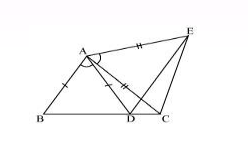
\includegraphics[width=\columnwidth]{figs/ABCDE.png}
	\caption{$\triangle ABC \hspace{12pt} and \hspace{12pt} \triangle ADE $}
 \label{fig:fig1}
\end{figure}
\textbf{Construction steps:}
		\begin{enumerate}[label=(\roman*)]
\item Let assume, the input parameters are, 
\begin{table}[H]
\centering
	\input{tables/table_1_bargav.tex}
	  \caption{Input Parameters}
	  \label{Table-1: }
\end{table}
$\therefore$ the output can be calculated as,
\begin{table}[H]
\centering
	\input{tables/table_2_bargav.tex}
	  \caption{Output Parameters}
	  \label{Table-2: }
\end{table}
$\therefore$ By, joining these points the required figure will be formed.
\begin{figure}[H]
    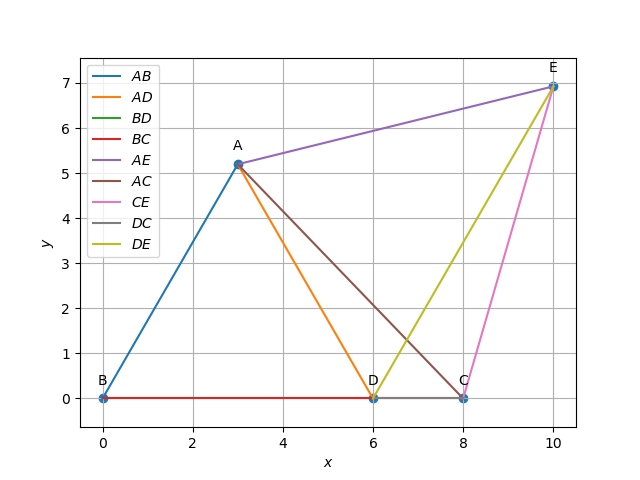
\includegraphics[width=\columnwidth]{figs/Final_python.png}
	\caption{$\triangle ABC \hspace{12pt} and \hspace{12pt} \triangle ADE$}
    \label{fig:fig2}
\end{figure}
\end{enumerate}
\end{enumerate}

\item 
	$AB$ is a line segment and $\vec{P}$ is its mid-point. $\vec{D}$ and $\vec{E}$ are points on the same side of
$AB$ such that $\angle BAD = \angle ABE$ and $\angle EPA = \angle DPB$. Show that
\label{chapters/9/7/1/7}
\begin{enumerate}
\item $\triangle DAP \cong \triangle EBP$
\item $AD = BE$.
\end{enumerate}
\solution
\begin{enumerate}[label=\thesection.\arabic*,ref=\thesection.\theenumi]
\numberwithin{equation}{enumi}
\numberwithin{figure}{enumi}
\numberwithin{table}{enumi}
\item Construct a triangle $ABC$ in which $BC=7cm, \angle{B}=75\degree$ and $AB + AC = 13 cm$.
\label{chapters/9/11/2/1}
%\input{chapters/9/11/2/1/line.tex}
%
\item Construct a triangle $ABC$ in which $BC=8cm, \angle{B}=45\degree$ and $AB - AC = 3.5 cm$.
\label{chapters/9/11/2/2}
\\
\solution
\input{chapters/9/11/2/2-new/vector-2.tex}
%
\item Construct a triangle $PQR$ in which $QR=6cm, \angle{Q}=60\degree$ and $PR - PQ = 2cm$.
\label{chapters/9/11/2/3}
%\input{chapters/9/11/2/3/line.tex}
%
\item Construct a triangle $XYZ$ in which $\angle{Y}=30\degree, \angle{Z}=90\degree$ and  $XY+YZ+ZX=11cm$.
\label{chapters/9/11/2/4}
%\input{chapters/9/11/2/4/line.tex}
%
\item Construct a right triangle whose base is 12cm and sum of its hypotenuse and other side is 18cm.
\label{chapters/9/11/2/5}
%\input{chapters/9/11/2/5/line.tex}
%
\item In Fig. \ref{fig:chapters/9/7/1/6/1}, $AC=AE,AB=AD$ and $\angle BAD=\angle EAC$. Show that $BC=DE$.
\label{chapters/9/7/1/6}
\begin{figure}[!h]
	\begin{center}
	\includegraphics[width=\columnwidth]{chapters/9/7/1/6/figs/fig.pdf}
	\end{center}
\caption{}
\label{fig:chapters/9/7/1/6/1}
\end{figure}
\\
\solution
\input{chapters/9/7/1/6/tri.tex}
\item 
	$AB$ is a line segment and $\vec{P}$ is its mid-point. $\vec{D}$ and $\vec{E}$ are points on the same side of
$AB$ such that $\angle BAD = \angle ABE$ and $\angle EPA = \angle DPB$. Show that
\label{chapters/9/7/1/7}
\begin{enumerate}
\item $\triangle DAP \cong \triangle EBP$
\item $AD = BE$.
\end{enumerate}
\solution
\input{chapters/9/7/1/7/tri.tex}
\item In right triangle ABC, right angled at C, M is the mid-point of hypotenuse AB. C is joined to M and produced to a point D such that DM = CM. Point D is joined to point B (see Figure \ref{fig:chapters/9/7/1/8/1}). Show that:
\begin{enumerate}
\item $\triangle AMC \cong \triangle BMD$
\item $\angle DBC$ is a right angle.
\item $\triangle DBC \cong \triangle ACB$
\item $CM = \dfrac{1}{2}AB$
\end{enumerate}
\label{chapters/9/7/1/8}
\input{chapters/9/7/1/8/vec.tex}
\item $AC = AE$ , $AB = AD$ and $\angle BAD = \angle EAC$. Show that $BC = DE$.
\begin{figure}[H]
    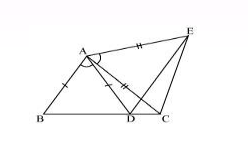
\includegraphics[width=\columnwidth]{figs/ABCDE.png}
	\caption{$\triangle ABC \hspace{12pt} and \hspace{12pt} \triangle ADE $}
 \label{fig:fig1}
\end{figure}
\textbf{Construction steps:}
		\begin{enumerate}[label=(\roman*)]
\item Let assume, the input parameters are, 
\begin{table}[H]
\centering
	\input{tables/table_1_bargav.tex}
	  \caption{Input Parameters}
	  \label{Table-1: }
\end{table}
$\therefore$ the output can be calculated as,
\begin{table}[H]
\centering
	\input{tables/table_2_bargav.tex}
	  \caption{Output Parameters}
	  \label{Table-2: }
\end{table}
$\therefore$ By, joining these points the required figure will be formed.
\begin{figure}[H]
    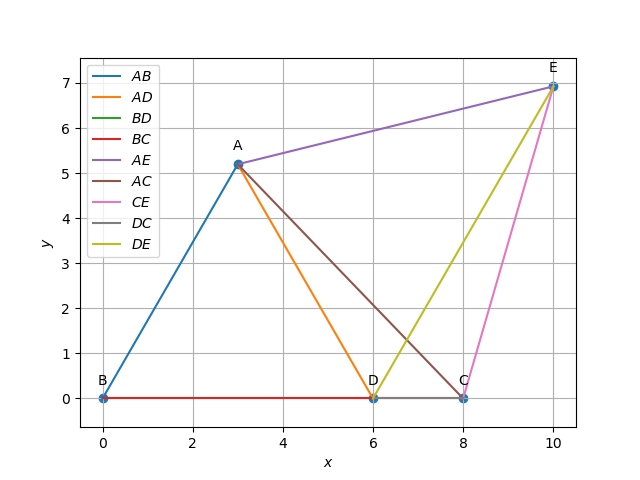
\includegraphics[width=\columnwidth]{figs/Final_python.png}
	\caption{$\triangle ABC \hspace{12pt} and \hspace{12pt} \triangle ADE$}
    \label{fig:fig2}
\end{figure}
\end{enumerate}
\end{enumerate}

\item In right triangle ABC, right angled at C, M is the mid-point of hypotenuse AB. C is joined to M and produced to a point D such that DM = CM. Point D is joined to point B (see Figure \ref{fig:chapters/9/7/1/8/1}). Show that:
\begin{enumerate}
\item $\triangle AMC \cong \triangle BMD$
\item $\angle DBC$ is a right angle.
\item $\triangle DBC \cong \triangle ACB$
\item $CM = \dfrac{1}{2}AB$
\end{enumerate}
\label{chapters/9/7/1/8}
\iffalse
\documentclass[10pt]{article}
\usepackage{graphicx}
\def\inputGnumericTable{}
\usepackage[latin1]{inputenc}
\usepackage{fullpage}
\usepackage{color}
\usepackage{array}
\usepackage{longtable}
\usepackage{calc}
\usepackage{multirow}
\usepackage{hhline}
\usepackage{ifthen}
\usepackage{amsmath}
\usepackage[none]{hyphenat}
\usepackage{listings}
\usepackage[english]{babel}
\usepackage{siunitx}
\usepackage{caption}
\usepackage{booktabs}
\usepackage{array}
\usepackage{extarrows}
\usepackage{enumerate}
\usepackage{enumitem}
\usepackage{amsmath}
\usepackage{commath}
\usepackage{gensymb}
\usepackage{amssymb}
\usepackage{multicol}
%\usepackage[utf8]{inputenc}
\lstset{
 frame=single,
 breaklines=true
}
\usepackage{hyperref}
\usepackage[margin=0.65in]{geometry}	 
%\usepackage{exsheets}% also loads the `tasks' package
\usepackage{atbegshi}
\AtBeginDocument{\AtBeginShipoutNext{\AtBeginShipoutDiscard}}

%new macro definitions
\renewcommand{\labelenumi}{(\roman{enumi})}
\newcommand{\mydet}[1]{\ensuremath{\begin{vmatrix}#1\end{vmatrix}}}
\providecommand{\brak}[1]{\ensuremath{\left(#1\right)}}
\newcommand{\solution}{\noindent \textbf{Solution: }}
\newcommand{\myvec}[1]{\ensuremath{\begin{pmatrix}#1\end{pmatrix}}}
\newenvironment{amatrix}[1]{%
	\left(\begin{array}{@{}*{#1}{c}|c@{}}
}{%
	\end{array}\right)
}

\newcommand{\myaugvec}[2]{\ensuremath{\begin{amatrix}{#1}#2\end{amatrix}}}
\providecommand{\norm}[1]{\left\1Vert#1\right\rVert}
\let\vec\mathbf{}


%\SetEnumitemKey{twocol}{
% before=\raggedcolumns\begin{multicols}{2},
% after=\end{multicols}}
%\SetEnumitemKey{fourcol}{
% before=\raggedcolumns\begin{multicols}{4},
% after=\end{multicols}} 


\begin{document}
\begin{center}
\title{\textbf{TRIANGLES}}
\date{\vspace{-5ex}}
\maketitle
\end{center}
\section*{9$^{th}$Math - Chapter 7}
This is Problem-8 from Exercise 7.1\\\\


\section*{\large Construction:}
\fi
The input parameters for construction
	are available in Table \ref{tab:chapters/9/7/1/8/table}.
\begin{table}[h!]
	\centering
	%\subimport{../chapters/9/7/1/8/tables/}{table.tex}
     \input{chapters/9/7/1/8/tables/table.tex}
	\caption{}
	\label{tab:chapters/9/7/1/8/table}
\end{table}
Thus, 
\begin{align}
	\vec{A}=\myvec{0\\b},\,
	\vec{B}=\myvec{a\\0},\,
	\vec{C}=\myvec{0\\0}
\end{align}
yielding
\begin{align}
	\vec{M}&=\frac{\vec{A}+\vec{B}}{2}=\frac{1}{2}\myvec{a\\b}
\end{align}
Also, 
\begin{align}
	\vec{M}&=\frac{\vec{C}+\vec{D}}{2}\\
	\implies \vec{D}&=2\vec{M}-\vec{C}=\myvec{a\\b}
\end{align}
\iffalse
\solution
Given
\begin{align}
	\vec{M}&=\frac{\vec{A}+\vec{B}}{2}
	\label{eq:chapters/9/7/1/8/1}\\
	\vec{D}-\vec{M}&=\vec{C}-\vec{M}
	\label{eq:chapters/9/7/1/8/2}\\
	\angle ACB&=90\degree
\end{align}
\textbf{Proof:} From Figure \ref{fig:chapters/9/7/1/8/1}
\fi
Thus,
\begin{align}
	\brak{\vec{D}-\vec{B}}^{\top}\brak{\vec{B}-\vec{C}} &= \myvec{0 & b}\myvec{a\\0}=0\\
	\implies BD & \perp BC\\
\end{align}
Also, 
\begin{align}
	\norm{\vec{A}-\vec{B}}&=\norm{\myvec{-a\\b}}\\
	\norm{\vec{C}-\vec{D}}&=\norm{\myvec{-a\\-b}}\\
	\implies \norm{\vec{A}-\vec{B}} &= \norm{\vec{C}-\vec{D}}\\
	\text{ or, } AB &= CD
	\label{eq:chapters/9/7/1/8/3}	
\end{align}
From \eqref{eq:chapters/9/7/1/8/3}
\begin{align}
	\implies CM = \frac{1}{2}CD = \frac{1}{2}AB 
\end{align}
See Fig. 
\ref{fig:chapters/9/7/1/8/1}.
\begin{figure}[H]
	\begin{center}
		\includegraphics[width=\columnwidth]{./chapters/9/7/1/8/figs/fig.pdf}
	\end{center}
\caption{}
\label{fig:chapters/9/7/1/8/1}
\end{figure}


\item $AC = AE$ , $AB = AD$ and $\angle BAD = \angle EAC$. Show that $BC = DE$.
\begin{figure}[H]
    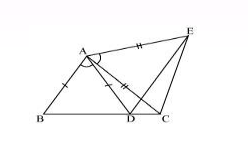
\includegraphics[width=\columnwidth]{figs/ABCDE.png}
	\caption{$\triangle ABC \hspace{12pt} and \hspace{12pt} \triangle ADE $}
 \label{fig:fig1}
\end{figure}
\textbf{Construction steps:}
		\begin{enumerate}[label=(\roman*)]
\item Let assume, the input parameters are, 
\begin{table}[H]
\centering
	\begin{tabular}{|c|c|p{5cm}|}
\hline
\textbf{Parameter} & \textbf{Value} & \textbf{Description} \\
\hline
	$\theta$ & $60\degree$ & $\angle{BAD} = \angle{CAE}$ \\
\hline
	$\vec{B}$ & $\myvec{0\\0}$ & Reference point at origin \\
\hline
	$\vec{D}$ & $\myvec{6\\0}$ & point $\vec{D}$ on the same axis of $\vec{B}$ \\
\hline
	$\vec{C}$ & $\myvec{8\\0}$ & point $\vec{C}$ on the same axis of $\vec{B}$ \\
\hline
\end{tabular}

	  \caption{Input Parameters}
	  \label{Table-1: }
\end{table}
$\therefore$ the output can be calculated as,
\begin{table}[H]
\centering
	\begin{tabular}{|c|c|p{5cm}|}
\hline
\textbf{Parameter} & \textbf{Value} & \textbf{Description} \\
\hline
	$BD$ & $\norm{\vec{B-D}}$ & Length of $BD$ \\
\hline
	$CD$ & $\norm{\vec{C-D}}$ & Length of $CD$ \\
\hline
	$\alpha$ & $\brak{\frac{180 - \theta}{2}}$ & $\angle ABD$ \\
\hline
	$AB$ & $BD \brak{\frac{\sin \alpha}{\sin \theta}}$ &  Length of $AB$ \\
\hline
	$\vec{A}$ & $\vec{B}$ + $\myvec{AB \cos \alpha  \\ AB \sin \alpha}$ & point $\vec{B}$ makes an angle $\alpha$  with line $(AB ,BD)$  \\
\hline
	$AD$ & $\norm{\vec{A-D}}$ & Length of $AD$ \\
\hline
	$AC$ & $\norm{\vec{A-C}}$ & Length of $AC$ \\
\hline
	  
	$\beta_1$ & $\cos^{-1} \brak{\frac{AC^2 +CD^2 - AD^2}{2 AC CD}}$ & $\angle ACD$ \\
\hline
	$CE$ & ${AC} \brak{\frac{\sin \theta}{\sin \alpha}}$ &  Length of $CE$ \\
\hline
	$\beta$ & $\alpha + \beta_1$ & $\angle ECB$\\

\hline
	$\vec{E}$ & $\vec{C}$ + $\myvec{-CE \cos \beta  \\ CE \sin \beta}$ & point $\vec{C}$ makes an angle $\beta$  with line $(BC ,CE)$  \\
\hline

\end{tabular}

	  \caption{Output Parameters}
	  \label{Table-2: }
\end{table}
$\therefore$ By, joining these points the required figure will be formed.
\begin{figure}[H]
    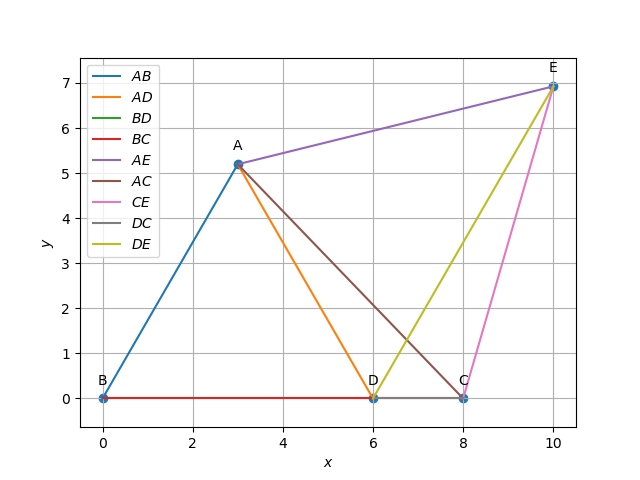
\includegraphics[width=\columnwidth]{figs/Final_python.png}
	\caption{$\triangle ABC \hspace{12pt} and \hspace{12pt} \triangle ADE$}
    \label{fig:fig2}
\end{figure}
\end{enumerate}
\end{enumerate}

\item In right triangle ABC, right angled at C, M is the mid-point of hypotenuse AB. C is joined to M and produced to a point D such that DM = CM. Point D is joined to point B (see Figure \ref{fig:chapters/9/7/1/8/1}). Show that:
\begin{enumerate}
\item $\triangle AMC \cong \triangle BMD$
\item $\angle DBC$ is a right angle.
\item $\triangle DBC \cong \triangle ACB$
\item $CM = \dfrac{1}{2}AB$
\end{enumerate}
\label{chapters/9/7/1/8}
\iffalse
\documentclass[10pt]{article}
\usepackage{graphicx}
\def\inputGnumericTable{}
\usepackage[latin1]{inputenc}
\usepackage{fullpage}
\usepackage{color}
\usepackage{array}
\usepackage{longtable}
\usepackage{calc}
\usepackage{multirow}
\usepackage{hhline}
\usepackage{ifthen}
\usepackage{amsmath}
\usepackage[none]{hyphenat}
\usepackage{listings}
\usepackage[english]{babel}
\usepackage{siunitx}
\usepackage{caption}
\usepackage{booktabs}
\usepackage{array}
\usepackage{extarrows}
\usepackage{enumerate}
\usepackage{enumitem}
\usepackage{amsmath}
\usepackage{commath}
\usepackage{gensymb}
\usepackage{amssymb}
\usepackage{multicol}
%\usepackage[utf8]{inputenc}
\lstset{
 frame=single,
 breaklines=true
}
\usepackage{hyperref}
\usepackage[margin=0.65in]{geometry}	 
%\usepackage{exsheets}% also loads the `tasks' package
\usepackage{atbegshi}
\AtBeginDocument{\AtBeginShipoutNext{\AtBeginShipoutDiscard}}

%new macro definitions
\renewcommand{\labelenumi}{(\roman{enumi})}
\newcommand{\mydet}[1]{\ensuremath{\begin{vmatrix}#1\end{vmatrix}}}
\providecommand{\brak}[1]{\ensuremath{\left(#1\right)}}
\newcommand{\solution}{\noindent \textbf{Solution: }}
\newcommand{\myvec}[1]{\ensuremath{\begin{pmatrix}#1\end{pmatrix}}}
\newenvironment{amatrix}[1]{%
	\left(\begin{array}{@{}*{#1}{c}|c@{}}
}{%
	\end{array}\right)
}

\newcommand{\myaugvec}[2]{\ensuremath{\begin{amatrix}{#1}#2\end{amatrix}}}
\providecommand{\norm}[1]{\left\1Vert#1\right\rVert}
\let\vec\mathbf{}


%\SetEnumitemKey{twocol}{
% before=\raggedcolumns\begin{multicols}{2},
% after=\end{multicols}}
%\SetEnumitemKey{fourcol}{
% before=\raggedcolumns\begin{multicols}{4},
% after=\end{multicols}} 


\begin{document}
\begin{center}
\title{\textbf{TRIANGLES}}
\date{\vspace{-5ex}}
\maketitle
\end{center}
\section*{9$^{th}$Math - Chapter 7}
This is Problem-8 from Exercise 7.1\\\\


\section*{\large Construction:}
\fi
The input parameters for construction
	are available in Table \ref{tab:chapters/9/7/1/8/table}.
\begin{table}[h!]
	\centering
	%\subimport{../chapters/9/7/1/8/tables/}{table.tex}
     \begin{tabular}{|c|c|p{5cm}|}
\hline
\textbf{Symbol} & \textbf{Value} & \textbf{Description} \\
\hline
$\theta$ & $30\degree$ & $\angle{BAP} = \angle{BAQ}$ \\
\hline
$a$ & $9$ & $AB$ \\
\hline
$c$ & $8$ & $AQ$ \\
\hline
$\vec{e}_1$ & $\myvec{1\\0}$ & Basis vector \\
\hline
\end{tabular}

	\caption{}
	\label{tab:chapters/9/7/1/8/table}
\end{table}
Thus, 
\begin{align}
	\vec{A}=\myvec{0\\b},\,
	\vec{B}=\myvec{a\\0},\,
	\vec{C}=\myvec{0\\0}
\end{align}
yielding
\begin{align}
	\vec{M}&=\frac{\vec{A}+\vec{B}}{2}=\frac{1}{2}\myvec{a\\b}
\end{align}
Also, 
\begin{align}
	\vec{M}&=\frac{\vec{C}+\vec{D}}{2}\\
	\implies \vec{D}&=2\vec{M}-\vec{C}=\myvec{a\\b}
\end{align}
\iffalse
\solution
Given
\begin{align}
	\vec{M}&=\frac{\vec{A}+\vec{B}}{2}
	\label{eq:chapters/9/7/1/8/1}\\
	\vec{D}-\vec{M}&=\vec{C}-\vec{M}
	\label{eq:chapters/9/7/1/8/2}\\
	\angle ACB&=90\degree
\end{align}
\textbf{Proof:} From Figure \ref{fig:chapters/9/7/1/8/1}
\fi
Thus,
\begin{align}
	\brak{\vec{D}-\vec{B}}^{\top}\brak{\vec{B}-\vec{C}} &= \myvec{0 & b}\myvec{a\\0}=0\\
	\implies BD & \perp BC\\
\end{align}
Also, 
\begin{align}
	\norm{\vec{A}-\vec{B}}&=\norm{\myvec{-a\\b}}\\
	\norm{\vec{C}-\vec{D}}&=\norm{\myvec{-a\\-b}}\\
	\implies \norm{\vec{A}-\vec{B}} &= \norm{\vec{C}-\vec{D}}\\
	\text{ or, } AB &= CD
	\label{eq:chapters/9/7/1/8/3}	
\end{align}
From \eqref{eq:chapters/9/7/1/8/3}
\begin{align}
	\implies CM = \frac{1}{2}CD = \frac{1}{2}AB 
\end{align}
See Fig. 
\ref{fig:chapters/9/7/1/8/1}.
\begin{figure}[H]
	\begin{center}
		\includegraphics[width=\columnwidth]{./chapters/9/7/1/8/figs/fig.pdf}
	\end{center}
\caption{}
\label{fig:chapters/9/7/1/8/1}
\end{figure}


\item $AC = AE$ , $AB = AD$ and $\angle BAD = \angle EAC$. Show that $BC = DE$.
\begin{figure}[H]
    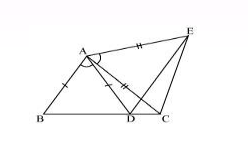
\includegraphics[width=\columnwidth]{figs/ABCDE.png}
	\caption{$\triangle ABC \hspace{12pt} and \hspace{12pt} \triangle ADE $}
 \label{fig:fig1}
\end{figure}
\textbf{Construction steps:}
		\begin{enumerate}[label=(\roman*)]
\item Let assume, the input parameters are, 
\begin{table}[H]
\centering
	\begin{tabular}{|c|c|p{5cm}|}
\hline
\textbf{Parameter} & \textbf{Value} & \textbf{Description} \\
\hline
	$\theta$ & $60\degree$ & $\angle{BAD} = \angle{CAE}$ \\
\hline
	$\vec{B}$ & $\myvec{0\\0}$ & Reference point at origin \\
\hline
	$\vec{D}$ & $\myvec{6\\0}$ & point $\vec{D}$ on the same axis of $\vec{B}$ \\
\hline
	$\vec{C}$ & $\myvec{8\\0}$ & point $\vec{C}$ on the same axis of $\vec{B}$ \\
\hline
\end{tabular}

	  \caption{Input Parameters}
	  \label{Table-1: }
\end{table}
$\therefore$ the output can be calculated as,
\begin{table}[H]
\centering
	\begin{tabular}{|c|c|p{5cm}|}
\hline
\textbf{Parameter} & \textbf{Value} & \textbf{Description} \\
\hline
	$BD$ & $\norm{\vec{B-D}}$ & Length of $BD$ \\
\hline
	$CD$ & $\norm{\vec{C-D}}$ & Length of $CD$ \\
\hline
	$\alpha$ & $\brak{\frac{180 - \theta}{2}}$ & $\angle ABD$ \\
\hline
	$AB$ & $BD \brak{\frac{\sin \alpha}{\sin \theta}}$ &  Length of $AB$ \\
\hline
	$\vec{A}$ & $\vec{B}$ + $\myvec{AB \cos \alpha  \\ AB \sin \alpha}$ & point $\vec{B}$ makes an angle $\alpha$  with line $(AB ,BD)$  \\
\hline
	$AD$ & $\norm{\vec{A-D}}$ & Length of $AD$ \\
\hline
	$AC$ & $\norm{\vec{A-C}}$ & Length of $AC$ \\
\hline
	  
	$\beta_1$ & $\cos^{-1} \brak{\frac{AC^2 +CD^2 - AD^2}{2 AC CD}}$ & $\angle ACD$ \\
\hline
	$CE$ & ${AC} \brak{\frac{\sin \theta}{\sin \alpha}}$ &  Length of $CE$ \\
\hline
	$\beta$ & $\alpha + \beta_1$ & $\angle ECB$\\

\hline
	$\vec{E}$ & $\vec{C}$ + $\myvec{-CE \cos \beta  \\ CE \sin \beta}$ & point $\vec{C}$ makes an angle $\beta$  with line $(BC ,CE)$  \\
\hline

\end{tabular}

	  \caption{Output Parameters}
	  \label{Table-2: }
\end{table}
$\therefore$ By, joining these points the required figure will be formed.
\begin{figure}[H]
    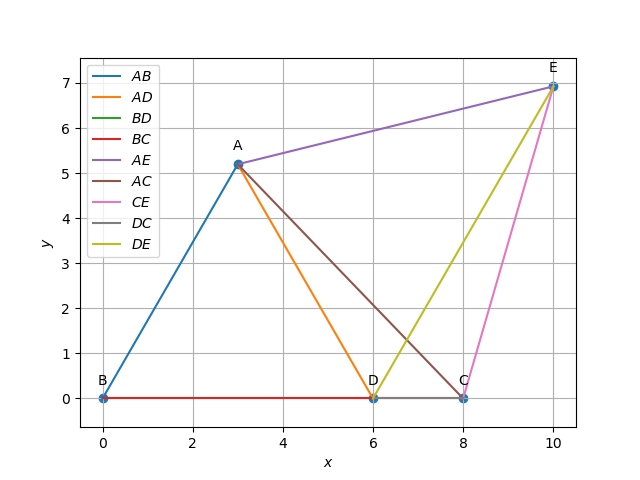
\includegraphics[width=\columnwidth]{figs/Final_python.png}
	\caption{$\triangle ABC \hspace{12pt} and \hspace{12pt} \triangle ADE$}
    \label{fig:fig2}
\end{figure}
\end{enumerate}
\end{enumerate}

\item 
	$AB$ is a line segment and $\vec{P}$ is its mid-point. $\vec{D}$ and $\vec{E}$ are points on the same side of
$AB$ such that $\angle BAD = \angle ABE$ and $\angle EPA = \angle DPB$. Show that
\label{chapters/9/7/1/7}
\begin{enumerate}
\item $\triangle DAP \cong \triangle EBP$
\item $AD = BE$.
\end{enumerate}
\solution
\begin{enumerate}[label=\thesection.\arabic*,ref=\thesection.\theenumi]
\numberwithin{equation}{enumi}
\numberwithin{figure}{enumi}
\numberwithin{table}{enumi}
\item Construct a triangle $ABC$ in which $BC=7cm, \angle{B}=75\degree$ and $AB + AC = 13 cm$.
\label{chapters/9/11/2/1}
%%\documentclass[12pt]{article}
%\usepackage[cmex10]{amsmath}
%\usepackage{amsthm}
%\usepackage{mathrsfs}
%\usepackage{txfonts}
%\usepackage{stfloats}
%\usepackage{bm}
%\usepackage{cite}
%\usepackage{cases}
%\usepackage{subfig}
%\usepackage{longtable}
%\usepackage{multirow}
%\usepackage{enumitem}
%\usepackage{mathtools}
%\usepackage{steinmetz}
%\usepackage{tikz}
%\usepackage{circuitikz}
%\usepackage{verbatim}
%\usepackage{tfrupee}
%\usepackage[breaklinks=true]{hyperref}
%\usepackage{tkz-euclide} % loads  TikZ and tkz-base
%\providecommand{\brak}[1]{\ensuremath{\left(#1\right)}}
%\usepackage{atbegshi}
%\AtBeginDocument{\AtBeginShipoutNext{\AtBeginShipoutDiscard}}
%\usetikzlibrary{calc,math}
%\usepackage{listings}
%    \usepackage{color}                                            %%
%    \usepackage{array}                                            %%
 %   \usepackage{longtable}                                        %%
  %  \usepackage{calc}                                             %%
   % \usepackage{multirow}                                         %%
    %\usepackage{hhline}                                           %%
    %\usepackage{ifthen}                                           %%
  %optionally (for landscape tables embedded in another document): %%
    %\usepackage{lscape}     
%\usepackage{multicol}
%\usepackage{chngcntr}

%\DeclareMathOperator*{\Res}{Res}
%\renewcommand{\baselinestretch}{2}
%\renewcommand\thesection{\arabic{section}}
%\renewcommand\thesubsection{\thesection.\arabic{subsection}}
%\renewcommand\thesubsubsection{\thesubsection.\arabic{subsubsection}}


% correct bad hyphenation here
%\hyphenation{op-tical net-works semi-conduc-tor}
%\def\inputGnumericTable{}                                 %%

%\lstset{
%language=C,
%frame=single, 
%breaklines=true,
%columns=fullflexible
%}
%\begin{document}
%\newtheorem{theorem}{Theorem}[section]
%\newtheorem{problem}{Problem}
%\newtheorem{proposition}{Proposition}[section]
%\newtheorem{lemma}{Lemma}[section]
%\newtheorem{corollary}[theorem]{Corollary}
%\newtheorem{example}{Example}[section]
%\newtheorem{definition}[problem]{Definition}
%\newcommand{\BEQA}{\begin{eqnarray}}
%\newcommand{\EEQA}{\end{eqnarray}}
%\newcommand{\define}{\stackrel{\triangle}{=}}

%\bibliographystyle{IEEEtran}
%\bibliographystyle{ieeetr}
%\providecommand{\mbf}{\mathbf}
%\providecommand{\pr}[1]{\ensuremath{\Pr\left(#1\right)}}
%\providecommand{\qfunc}[1]{\ensuremath{Q\left(#1\right)}}
%\providecommand{\sbrak}[1]{\ensuremath{{}\left[#1\right]}}
%\providecommand{\lsbrak}[1]{\ensuremath{{}\left[#1\right.}}
%\providecommand{\rsbrak}[1]{\ensuremath{{}\left.#1\right]}}
%\providecommand{\brak}[1]{\ensuremath{\left(#1\right)}}
%\providecommand{\lbrak}[1]{\ensuremath{\left(#1\right.}}
%\providecommand{\rbrak}[1]{\ensuremath{\left.#1\right)}}
%\providecommand{\cbrak}[1]{\ensuremath{\left\{#1\right\}}}
%\providecommand{\lcbrak}[1]{\ensuremath{\left\{#1\right.}}
%\providecommand{\rcbrak}[1]{\ensuremath{\left.#1\right\}}}
%\theoremstyle{remark}
%\newtheorem{rem}{Remark}
%\newcommand{\sgn}{\mathop{\mathrm{sgn}}}
%\providecommand{\res}[1]{\Res\displaylimits_{#1}} 
%\providecommand{\mtx}[1]{\mathbf{#1}}
%\providecommand{\fourier}{\overset{\mathcal{F}}{\rightleftharpoons}}
%\providecommand{\system}{\overset{\mathcal{H}}{\longleftrightarrow}}
	%\newcommand{\solution}[2]{\textbf{Solution:}{#1}}
%\newcommand{\solution}{\noindent \textbf{Solution: }}
%\newcommand{\cosec}{\,\text{cosec}\,}
%\providecommand{\dec}[2]{\ensuremath{\overset{#1}{\underset{#2}{\gtrless}}}}
%\newcommand{\myvec}[1]{\ensuremath{\begin{pmatrix}#1\end{pmatrix}}}
%\newcommand{\mydet}[1]{\ensuremath{\begin{vmatrix}#1\end{vmatrix}}}
%\let\vec\mathbf
%\begin{center}
%\title{\textbf{Straight Lines}}
%\date{\vspace{-5ex}} %Not to print date automatically
%\maketitle
%\end{center}
%\setcounter{page}{1}
%\section*{11$^{th}$ Maths - Chapter 10}
%This is Problem-10 from Exercise 10.4
%\begin{enumerate}
%    \item If three lines whose equations are $y=m_1x+c_1$, $y=m_2x+c_2$ and $y=m_3x+c_3$ are concurrent, then show that $m_1(c_2-c_3)+m_2(c_3-c_1)+m_3(c_1-c_2) = 0.$\\
%    \solution 
    Given lines can be written as \begin{align}
       m_1x-y+c_1=0
    \end{align}
    \begin{align}
        m_2x-y+c_2=0
    \end{align}
    \begin{align}
        m_3x-y+c_3=0
        \label{eq:3}
    \end{align}
    
    
   The above lines can be written in the form of \begin{align}
        \Vec{n}^{\top}\Vec{x} = c
    \end{align}
   Therefore,
		\begin{align}
       \myvec{m_1&-1}\vec{x}=c_1
       \label{eq:5}
   \end{align} 
   \begin{align}
       \myvec{m_2&-1}\vec{x}=c_2
       \label{eq:6}
   \end{align}
   \begin{align}
       \myvec{m_3&-1}\vec{x}=c_3
       \label{eq:7}
   \end{align}
   Solving equations \eqref{eq:5}, \eqref{eq:6}and \eqref{eq:7}
		augumented matrix is
 \begin{align}
    \myvec{m_1&-1&c_1\\m_2&-1&c_2\\m_3&-1&c_3}\\
    \xleftrightarrow{R_2 \leftarrow m_1R_2-m_2R_1}
    \myvec{m_1&-1&c_1\\0&m_2-m_1&m_1c_2-m_2c_1\\m_3&-1&c_3}\\
    \xleftrightarrow{R_3 \leftarrow m_1R_3-m_3R_1}
    \myvec{m_1&-1&c_1\\0&m_2-m_1&m_1c_2-m_2c_1\\0&m_3-m_1&m_1c_3-m_3c_1}\\
    \xleftrightarrow{R_3 \leftarrow R_3\frac{m_2-m_1}{m_3-m_1}-R_2}
        \myvec{m_1&-1&c_1\\0&m_2-m_1&m_1c_2-m_2c_1\\0&0&$\brak{m_1c_3-m_3c_1}$$\brak{\frac{m_2-m_1}{m_3-m_1}}$-$\brak{m_1c_2-m_2c_1}$}
\end{align}
Now, for lines to be concurrent, then the third row should be equal to zero. \\

Therefore,
\begin{align}
\brak{m_1c_3-m_3c_1}\brak{\frac{m_2-m_1}{m_3-m_1}}-\brak{m_1c_2-m_2c_1}=0\\
\frac{\brak{m_1c_3-m_3c_1}\brak{m_2-m_1}-\brak{m_1c_2-m_2c_1}\brak{m_3-m_1}}{m_3-m_1}=0\\
\brak{m_1c_3-m_3c_1}\brak{m_2-m_1}-\brak{m_1c_2-m_2c_1}\brak{m_3-m_1}=0\\
m_2c_3-m_1c_3+m_3c_1-m_3c_2+m_1c_2-m_2c_1=0\\
m_1\brak{c_2-c_3}+m_2\brak{c_3-c_1}+m_3\brak{c_1-c_2} = 0
\end{align}
           Hence proved
%\begin{figure}[h]
 %   \centering
  %  \includegraphics[width=\columnwidth]{concurrent-1.png}
   % \caption{Straight Lines}
    %\label{fig:concurrent-1.png}
%\end{figure}
%\end{enumerate}
%\end{document}

%
\item Construct a triangle $ABC$ in which $BC=8cm, \angle{B}=45\degree$ and $AB - AC = 3.5 cm$.
\label{chapters/9/11/2/2}
\\
\solution
\input{chapters/9/11/2/2-new/vector-2.tex}
%
\item Construct a triangle $PQR$ in which $QR=6cm, \angle{Q}=60\degree$ and $PR - PQ = 2cm$.
\label{chapters/9/11/2/3}
%%\documentclass[12pt]{article}
%\usepackage[cmex10]{amsmath}
%\usepackage{amsthm}
%\usepackage{mathrsfs}
%\usepackage{txfonts}
%\usepackage{stfloats}
%\usepackage{bm}
%\usepackage{cite}
%\usepackage{cases}
%\usepackage{subfig}
%\usepackage{longtable}
%\usepackage{multirow}
%\usepackage{enumitem}
%\usepackage{mathtools}
%\usepackage{steinmetz}
%\usepackage{tikz}
%\usepackage{circuitikz}
%\usepackage{verbatim}
%\usepackage{tfrupee}
%\usepackage[breaklinks=true]{hyperref}
%\usepackage{tkz-euclide} % loads  TikZ and tkz-base
%\providecommand{\brak}[1]{\ensuremath{\left(#1\right)}}
%\usepackage{atbegshi}
%\AtBeginDocument{\AtBeginShipoutNext{\AtBeginShipoutDiscard}}
%\usetikzlibrary{calc,math}
%\usepackage{listings}
%    \usepackage{color}                                            %%
%    \usepackage{array}                                            %%
 %   \usepackage{longtable}                                        %%
  %  \usepackage{calc}                                             %%
   % \usepackage{multirow}                                         %%
    %\usepackage{hhline}                                           %%
    %\usepackage{ifthen}                                           %%
  %optionally (for landscape tables embedded in another document): %%
    %\usepackage{lscape}     
%\usepackage{multicol}
%\usepackage{chngcntr}

%\DeclareMathOperator*{\Res}{Res}
%\renewcommand{\baselinestretch}{2}
%\renewcommand\thesection{\arabic{section}}
%\renewcommand\thesubsection{\thesection.\arabic{subsection}}
%\renewcommand\thesubsubsection{\thesubsection.\arabic{subsubsection}}


% correct bad hyphenation here
%\hyphenation{op-tical net-works semi-conduc-tor}
%\def\inputGnumericTable{}                                 %%

%\lstset{
%language=C,
%frame=single, 
%breaklines=true,
%columns=fullflexible
%}
%\begin{document}
%\newtheorem{theorem}{Theorem}[section]
%\newtheorem{problem}{Problem}
%\newtheorem{proposition}{Proposition}[section]
%\newtheorem{lemma}{Lemma}[section]
%\newtheorem{corollary}[theorem]{Corollary}
%\newtheorem{example}{Example}[section]
%\newtheorem{definition}[problem]{Definition}
%\newcommand{\BEQA}{\begin{eqnarray}}
%\newcommand{\EEQA}{\end{eqnarray}}
%\newcommand{\define}{\stackrel{\triangle}{=}}

%\bibliographystyle{IEEEtran}
%\bibliographystyle{ieeetr}
%\providecommand{\mbf}{\mathbf}
%\providecommand{\pr}[1]{\ensuremath{\Pr\left(#1\right)}}
%\providecommand{\qfunc}[1]{\ensuremath{Q\left(#1\right)}}
%\providecommand{\sbrak}[1]{\ensuremath{{}\left[#1\right]}}
%\providecommand{\lsbrak}[1]{\ensuremath{{}\left[#1\right.}}
%\providecommand{\rsbrak}[1]{\ensuremath{{}\left.#1\right]}}
%\providecommand{\brak}[1]{\ensuremath{\left(#1\right)}}
%\providecommand{\lbrak}[1]{\ensuremath{\left(#1\right.}}
%\providecommand{\rbrak}[1]{\ensuremath{\left.#1\right)}}
%\providecommand{\cbrak}[1]{\ensuremath{\left\{#1\right\}}}
%\providecommand{\lcbrak}[1]{\ensuremath{\left\{#1\right.}}
%\providecommand{\rcbrak}[1]{\ensuremath{\left.#1\right\}}}
%\theoremstyle{remark}
%\newtheorem{rem}{Remark}
%\newcommand{\sgn}{\mathop{\mathrm{sgn}}}
%\providecommand{\res}[1]{\Res\displaylimits_{#1}} 
%\providecommand{\mtx}[1]{\mathbf{#1}}
%\providecommand{\fourier}{\overset{\mathcal{F}}{\rightleftharpoons}}
%\providecommand{\system}{\overset{\mathcal{H}}{\longleftrightarrow}}
	%\newcommand{\solution}[2]{\textbf{Solution:}{#1}}
%\newcommand{\solution}{\noindent \textbf{Solution: }}
%\newcommand{\cosec}{\,\text{cosec}\,}
%\providecommand{\dec}[2]{\ensuremath{\overset{#1}{\underset{#2}{\gtrless}}}}
%\newcommand{\myvec}[1]{\ensuremath{\begin{pmatrix}#1\end{pmatrix}}}
%\newcommand{\mydet}[1]{\ensuremath{\begin{vmatrix}#1\end{vmatrix}}}
%\let\vec\mathbf
%\begin{center}
%\title{\textbf{Straight Lines}}
%\date{\vspace{-5ex}} %Not to print date automatically
%\maketitle
%\end{center}
%\setcounter{page}{1}
%\section*{11$^{th}$ Maths - Chapter 10}
%This is Problem-10 from Exercise 10.4
%\begin{enumerate}
%    \item If three lines whose equations are $y=m_1x+c_1$, $y=m_2x+c_2$ and $y=m_3x+c_3$ are concurrent, then show that $m_1(c_2-c_3)+m_2(c_3-c_1)+m_3(c_1-c_2) = 0.$\\
%    \solution 
    Given lines can be written as \begin{align}
       m_1x-y+c_1=0
    \end{align}
    \begin{align}
        m_2x-y+c_2=0
    \end{align}
    \begin{align}
        m_3x-y+c_3=0
        \label{eq:3}
    \end{align}
    
    
   The above lines can be written in the form of \begin{align}
        \Vec{n}^{\top}\Vec{x} = c
    \end{align}
   Therefore,
		\begin{align}
       \myvec{m_1&-1}\vec{x}=c_1
       \label{eq:5}
   \end{align} 
   \begin{align}
       \myvec{m_2&-1}\vec{x}=c_2
       \label{eq:6}
   \end{align}
   \begin{align}
       \myvec{m_3&-1}\vec{x}=c_3
       \label{eq:7}
   \end{align}
   Solving equations \eqref{eq:5}, \eqref{eq:6}and \eqref{eq:7}
		augumented matrix is
 \begin{align}
    \myvec{m_1&-1&c_1\\m_2&-1&c_2\\m_3&-1&c_3}\\
    \xleftrightarrow{R_2 \leftarrow m_1R_2-m_2R_1}
    \myvec{m_1&-1&c_1\\0&m_2-m_1&m_1c_2-m_2c_1\\m_3&-1&c_3}\\
    \xleftrightarrow{R_3 \leftarrow m_1R_3-m_3R_1}
    \myvec{m_1&-1&c_1\\0&m_2-m_1&m_1c_2-m_2c_1\\0&m_3-m_1&m_1c_3-m_3c_1}\\
    \xleftrightarrow{R_3 \leftarrow R_3\frac{m_2-m_1}{m_3-m_1}-R_2}
        \myvec{m_1&-1&c_1\\0&m_2-m_1&m_1c_2-m_2c_1\\0&0&$\brak{m_1c_3-m_3c_1}$$\brak{\frac{m_2-m_1}{m_3-m_1}}$-$\brak{m_1c_2-m_2c_1}$}
\end{align}
Now, for lines to be concurrent, then the third row should be equal to zero. \\

Therefore,
\begin{align}
\brak{m_1c_3-m_3c_1}\brak{\frac{m_2-m_1}{m_3-m_1}}-\brak{m_1c_2-m_2c_1}=0\\
\frac{\brak{m_1c_3-m_3c_1}\brak{m_2-m_1}-\brak{m_1c_2-m_2c_1}\brak{m_3-m_1}}{m_3-m_1}=0\\
\brak{m_1c_3-m_3c_1}\brak{m_2-m_1}-\brak{m_1c_2-m_2c_1}\brak{m_3-m_1}=0\\
m_2c_3-m_1c_3+m_3c_1-m_3c_2+m_1c_2-m_2c_1=0\\
m_1\brak{c_2-c_3}+m_2\brak{c_3-c_1}+m_3\brak{c_1-c_2} = 0
\end{align}
           Hence proved
%\begin{figure}[h]
 %   \centering
  %  \includegraphics[width=\columnwidth]{concurrent-1.png}
   % \caption{Straight Lines}
    %\label{fig:concurrent-1.png}
%\end{figure}
%\end{enumerate}
%\end{document}

%
\item Construct a triangle $XYZ$ in which $\angle{Y}=30\degree, \angle{Z}=90\degree$ and  $XY+YZ+ZX=11cm$.
\label{chapters/9/11/2/4}
%%\documentclass[12pt]{article}
%\usepackage[cmex10]{amsmath}
%\usepackage{amsthm}
%\usepackage{mathrsfs}
%\usepackage{txfonts}
%\usepackage{stfloats}
%\usepackage{bm}
%\usepackage{cite}
%\usepackage{cases}
%\usepackage{subfig}
%\usepackage{longtable}
%\usepackage{multirow}
%\usepackage{enumitem}
%\usepackage{mathtools}
%\usepackage{steinmetz}
%\usepackage{tikz}
%\usepackage{circuitikz}
%\usepackage{verbatim}
%\usepackage{tfrupee}
%\usepackage[breaklinks=true]{hyperref}
%\usepackage{tkz-euclide} % loads  TikZ and tkz-base
%\providecommand{\brak}[1]{\ensuremath{\left(#1\right)}}
%\usepackage{atbegshi}
%\AtBeginDocument{\AtBeginShipoutNext{\AtBeginShipoutDiscard}}
%\usetikzlibrary{calc,math}
%\usepackage{listings}
%    \usepackage{color}                                            %%
%    \usepackage{array}                                            %%
 %   \usepackage{longtable}                                        %%
  %  \usepackage{calc}                                             %%
   % \usepackage{multirow}                                         %%
    %\usepackage{hhline}                                           %%
    %\usepackage{ifthen}                                           %%
  %optionally (for landscape tables embedded in another document): %%
    %\usepackage{lscape}     
%\usepackage{multicol}
%\usepackage{chngcntr}

%\DeclareMathOperator*{\Res}{Res}
%\renewcommand{\baselinestretch}{2}
%\renewcommand\thesection{\arabic{section}}
%\renewcommand\thesubsection{\thesection.\arabic{subsection}}
%\renewcommand\thesubsubsection{\thesubsection.\arabic{subsubsection}}


% correct bad hyphenation here
%\hyphenation{op-tical net-works semi-conduc-tor}
%\def\inputGnumericTable{}                                 %%

%\lstset{
%language=C,
%frame=single, 
%breaklines=true,
%columns=fullflexible
%}
%\begin{document}
%\newtheorem{theorem}{Theorem}[section]
%\newtheorem{problem}{Problem}
%\newtheorem{proposition}{Proposition}[section]
%\newtheorem{lemma}{Lemma}[section]
%\newtheorem{corollary}[theorem]{Corollary}
%\newtheorem{example}{Example}[section]
%\newtheorem{definition}[problem]{Definition}
%\newcommand{\BEQA}{\begin{eqnarray}}
%\newcommand{\EEQA}{\end{eqnarray}}
%\newcommand{\define}{\stackrel{\triangle}{=}}

%\bibliographystyle{IEEEtran}
%\bibliographystyle{ieeetr}
%\providecommand{\mbf}{\mathbf}
%\providecommand{\pr}[1]{\ensuremath{\Pr\left(#1\right)}}
%\providecommand{\qfunc}[1]{\ensuremath{Q\left(#1\right)}}
%\providecommand{\sbrak}[1]{\ensuremath{{}\left[#1\right]}}
%\providecommand{\lsbrak}[1]{\ensuremath{{}\left[#1\right.}}
%\providecommand{\rsbrak}[1]{\ensuremath{{}\left.#1\right]}}
%\providecommand{\brak}[1]{\ensuremath{\left(#1\right)}}
%\providecommand{\lbrak}[1]{\ensuremath{\left(#1\right.}}
%\providecommand{\rbrak}[1]{\ensuremath{\left.#1\right)}}
%\providecommand{\cbrak}[1]{\ensuremath{\left\{#1\right\}}}
%\providecommand{\lcbrak}[1]{\ensuremath{\left\{#1\right.}}
%\providecommand{\rcbrak}[1]{\ensuremath{\left.#1\right\}}}
%\theoremstyle{remark}
%\newtheorem{rem}{Remark}
%\newcommand{\sgn}{\mathop{\mathrm{sgn}}}
%\providecommand{\res}[1]{\Res\displaylimits_{#1}} 
%\providecommand{\mtx}[1]{\mathbf{#1}}
%\providecommand{\fourier}{\overset{\mathcal{F}}{\rightleftharpoons}}
%\providecommand{\system}{\overset{\mathcal{H}}{\longleftrightarrow}}
	%\newcommand{\solution}[2]{\textbf{Solution:}{#1}}
%\newcommand{\solution}{\noindent \textbf{Solution: }}
%\newcommand{\cosec}{\,\text{cosec}\,}
%\providecommand{\dec}[2]{\ensuremath{\overset{#1}{\underset{#2}{\gtrless}}}}
%\newcommand{\myvec}[1]{\ensuremath{\begin{pmatrix}#1\end{pmatrix}}}
%\newcommand{\mydet}[1]{\ensuremath{\begin{vmatrix}#1\end{vmatrix}}}
%\let\vec\mathbf
%\begin{center}
%\title{\textbf{Straight Lines}}
%\date{\vspace{-5ex}} %Not to print date automatically
%\maketitle
%\end{center}
%\setcounter{page}{1}
%\section*{11$^{th}$ Maths - Chapter 10}
%This is Problem-10 from Exercise 10.4
%\begin{enumerate}
%    \item If three lines whose equations are $y=m_1x+c_1$, $y=m_2x+c_2$ and $y=m_3x+c_3$ are concurrent, then show that $m_1(c_2-c_3)+m_2(c_3-c_1)+m_3(c_1-c_2) = 0.$\\
%    \solution 
    Given lines can be written as \begin{align}
       m_1x-y+c_1=0
    \end{align}
    \begin{align}
        m_2x-y+c_2=0
    \end{align}
    \begin{align}
        m_3x-y+c_3=0
        \label{eq:3}
    \end{align}
    
    
   The above lines can be written in the form of \begin{align}
        \Vec{n}^{\top}\Vec{x} = c
    \end{align}
   Therefore,
		\begin{align}
       \myvec{m_1&-1}\vec{x}=c_1
       \label{eq:5}
   \end{align} 
   \begin{align}
       \myvec{m_2&-1}\vec{x}=c_2
       \label{eq:6}
   \end{align}
   \begin{align}
       \myvec{m_3&-1}\vec{x}=c_3
       \label{eq:7}
   \end{align}
   Solving equations \eqref{eq:5}, \eqref{eq:6}and \eqref{eq:7}
		augumented matrix is
 \begin{align}
    \myvec{m_1&-1&c_1\\m_2&-1&c_2\\m_3&-1&c_3}\\
    \xleftrightarrow{R_2 \leftarrow m_1R_2-m_2R_1}
    \myvec{m_1&-1&c_1\\0&m_2-m_1&m_1c_2-m_2c_1\\m_3&-1&c_3}\\
    \xleftrightarrow{R_3 \leftarrow m_1R_3-m_3R_1}
    \myvec{m_1&-1&c_1\\0&m_2-m_1&m_1c_2-m_2c_1\\0&m_3-m_1&m_1c_3-m_3c_1}\\
    \xleftrightarrow{R_3 \leftarrow R_3\frac{m_2-m_1}{m_3-m_1}-R_2}
        \myvec{m_1&-1&c_1\\0&m_2-m_1&m_1c_2-m_2c_1\\0&0&$\brak{m_1c_3-m_3c_1}$$\brak{\frac{m_2-m_1}{m_3-m_1}}$-$\brak{m_1c_2-m_2c_1}$}
\end{align}
Now, for lines to be concurrent, then the third row should be equal to zero. \\

Therefore,
\begin{align}
\brak{m_1c_3-m_3c_1}\brak{\frac{m_2-m_1}{m_3-m_1}}-\brak{m_1c_2-m_2c_1}=0\\
\frac{\brak{m_1c_3-m_3c_1}\brak{m_2-m_1}-\brak{m_1c_2-m_2c_1}\brak{m_3-m_1}}{m_3-m_1}=0\\
\brak{m_1c_3-m_3c_1}\brak{m_2-m_1}-\brak{m_1c_2-m_2c_1}\brak{m_3-m_1}=0\\
m_2c_3-m_1c_3+m_3c_1-m_3c_2+m_1c_2-m_2c_1=0\\
m_1\brak{c_2-c_3}+m_2\brak{c_3-c_1}+m_3\brak{c_1-c_2} = 0
\end{align}
           Hence proved
%\begin{figure}[h]
 %   \centering
  %  \includegraphics[width=\columnwidth]{concurrent-1.png}
   % \caption{Straight Lines}
    %\label{fig:concurrent-1.png}
%\end{figure}
%\end{enumerate}
%\end{document}

%
\item Construct a right triangle whose base is 12cm and sum of its hypotenuse and other side is 18cm.
\label{chapters/9/11/2/5}
%%\documentclass[12pt]{article}
%\usepackage[cmex10]{amsmath}
%\usepackage{amsthm}
%\usepackage{mathrsfs}
%\usepackage{txfonts}
%\usepackage{stfloats}
%\usepackage{bm}
%\usepackage{cite}
%\usepackage{cases}
%\usepackage{subfig}
%\usepackage{longtable}
%\usepackage{multirow}
%\usepackage{enumitem}
%\usepackage{mathtools}
%\usepackage{steinmetz}
%\usepackage{tikz}
%\usepackage{circuitikz}
%\usepackage{verbatim}
%\usepackage{tfrupee}
%\usepackage[breaklinks=true]{hyperref}
%\usepackage{tkz-euclide} % loads  TikZ and tkz-base
%\providecommand{\brak}[1]{\ensuremath{\left(#1\right)}}
%\usepackage{atbegshi}
%\AtBeginDocument{\AtBeginShipoutNext{\AtBeginShipoutDiscard}}
%\usetikzlibrary{calc,math}
%\usepackage{listings}
%    \usepackage{color}                                            %%
%    \usepackage{array}                                            %%
 %   \usepackage{longtable}                                        %%
  %  \usepackage{calc}                                             %%
   % \usepackage{multirow}                                         %%
    %\usepackage{hhline}                                           %%
    %\usepackage{ifthen}                                           %%
  %optionally (for landscape tables embedded in another document): %%
    %\usepackage{lscape}     
%\usepackage{multicol}
%\usepackage{chngcntr}

%\DeclareMathOperator*{\Res}{Res}
%\renewcommand{\baselinestretch}{2}
%\renewcommand\thesection{\arabic{section}}
%\renewcommand\thesubsection{\thesection.\arabic{subsection}}
%\renewcommand\thesubsubsection{\thesubsection.\arabic{subsubsection}}


% correct bad hyphenation here
%\hyphenation{op-tical net-works semi-conduc-tor}
%\def\inputGnumericTable{}                                 %%

%\lstset{
%language=C,
%frame=single, 
%breaklines=true,
%columns=fullflexible
%}
%\begin{document}
%\newtheorem{theorem}{Theorem}[section]
%\newtheorem{problem}{Problem}
%\newtheorem{proposition}{Proposition}[section]
%\newtheorem{lemma}{Lemma}[section]
%\newtheorem{corollary}[theorem]{Corollary}
%\newtheorem{example}{Example}[section]
%\newtheorem{definition}[problem]{Definition}
%\newcommand{\BEQA}{\begin{eqnarray}}
%\newcommand{\EEQA}{\end{eqnarray}}
%\newcommand{\define}{\stackrel{\triangle}{=}}

%\bibliographystyle{IEEEtran}
%\bibliographystyle{ieeetr}
%\providecommand{\mbf}{\mathbf}
%\providecommand{\pr}[1]{\ensuremath{\Pr\left(#1\right)}}
%\providecommand{\qfunc}[1]{\ensuremath{Q\left(#1\right)}}
%\providecommand{\sbrak}[1]{\ensuremath{{}\left[#1\right]}}
%\providecommand{\lsbrak}[1]{\ensuremath{{}\left[#1\right.}}
%\providecommand{\rsbrak}[1]{\ensuremath{{}\left.#1\right]}}
%\providecommand{\brak}[1]{\ensuremath{\left(#1\right)}}
%\providecommand{\lbrak}[1]{\ensuremath{\left(#1\right.}}
%\providecommand{\rbrak}[1]{\ensuremath{\left.#1\right)}}
%\providecommand{\cbrak}[1]{\ensuremath{\left\{#1\right\}}}
%\providecommand{\lcbrak}[1]{\ensuremath{\left\{#1\right.}}
%\providecommand{\rcbrak}[1]{\ensuremath{\left.#1\right\}}}
%\theoremstyle{remark}
%\newtheorem{rem}{Remark}
%\newcommand{\sgn}{\mathop{\mathrm{sgn}}}
%\providecommand{\res}[1]{\Res\displaylimits_{#1}} 
%\providecommand{\mtx}[1]{\mathbf{#1}}
%\providecommand{\fourier}{\overset{\mathcal{F}}{\rightleftharpoons}}
%\providecommand{\system}{\overset{\mathcal{H}}{\longleftrightarrow}}
	%\newcommand{\solution}[2]{\textbf{Solution:}{#1}}
%\newcommand{\solution}{\noindent \textbf{Solution: }}
%\newcommand{\cosec}{\,\text{cosec}\,}
%\providecommand{\dec}[2]{\ensuremath{\overset{#1}{\underset{#2}{\gtrless}}}}
%\newcommand{\myvec}[1]{\ensuremath{\begin{pmatrix}#1\end{pmatrix}}}
%\newcommand{\mydet}[1]{\ensuremath{\begin{vmatrix}#1\end{vmatrix}}}
%\let\vec\mathbf
%\begin{center}
%\title{\textbf{Straight Lines}}
%\date{\vspace{-5ex}} %Not to print date automatically
%\maketitle
%\end{center}
%\setcounter{page}{1}
%\section*{11$^{th}$ Maths - Chapter 10}
%This is Problem-10 from Exercise 10.4
%\begin{enumerate}
%    \item If three lines whose equations are $y=m_1x+c_1$, $y=m_2x+c_2$ and $y=m_3x+c_3$ are concurrent, then show that $m_1(c_2-c_3)+m_2(c_3-c_1)+m_3(c_1-c_2) = 0.$\\
%    \solution 
    Given lines can be written as \begin{align}
       m_1x-y+c_1=0
    \end{align}
    \begin{align}
        m_2x-y+c_2=0
    \end{align}
    \begin{align}
        m_3x-y+c_3=0
        \label{eq:3}
    \end{align}
    
    
   The above lines can be written in the form of \begin{align}
        \Vec{n}^{\top}\Vec{x} = c
    \end{align}
   Therefore,
		\begin{align}
       \myvec{m_1&-1}\vec{x}=c_1
       \label{eq:5}
   \end{align} 
   \begin{align}
       \myvec{m_2&-1}\vec{x}=c_2
       \label{eq:6}
   \end{align}
   \begin{align}
       \myvec{m_3&-1}\vec{x}=c_3
       \label{eq:7}
   \end{align}
   Solving equations \eqref{eq:5}, \eqref{eq:6}and \eqref{eq:7}
		augumented matrix is
 \begin{align}
    \myvec{m_1&-1&c_1\\m_2&-1&c_2\\m_3&-1&c_3}\\
    \xleftrightarrow{R_2 \leftarrow m_1R_2-m_2R_1}
    \myvec{m_1&-1&c_1\\0&m_2-m_1&m_1c_2-m_2c_1\\m_3&-1&c_3}\\
    \xleftrightarrow{R_3 \leftarrow m_1R_3-m_3R_1}
    \myvec{m_1&-1&c_1\\0&m_2-m_1&m_1c_2-m_2c_1\\0&m_3-m_1&m_1c_3-m_3c_1}\\
    \xleftrightarrow{R_3 \leftarrow R_3\frac{m_2-m_1}{m_3-m_1}-R_2}
        \myvec{m_1&-1&c_1\\0&m_2-m_1&m_1c_2-m_2c_1\\0&0&$\brak{m_1c_3-m_3c_1}$$\brak{\frac{m_2-m_1}{m_3-m_1}}$-$\brak{m_1c_2-m_2c_1}$}
\end{align}
Now, for lines to be concurrent, then the third row should be equal to zero. \\

Therefore,
\begin{align}
\brak{m_1c_3-m_3c_1}\brak{\frac{m_2-m_1}{m_3-m_1}}-\brak{m_1c_2-m_2c_1}=0\\
\frac{\brak{m_1c_3-m_3c_1}\brak{m_2-m_1}-\brak{m_1c_2-m_2c_1}\brak{m_3-m_1}}{m_3-m_1}=0\\
\brak{m_1c_3-m_3c_1}\brak{m_2-m_1}-\brak{m_1c_2-m_2c_1}\brak{m_3-m_1}=0\\
m_2c_3-m_1c_3+m_3c_1-m_3c_2+m_1c_2-m_2c_1=0\\
m_1\brak{c_2-c_3}+m_2\brak{c_3-c_1}+m_3\brak{c_1-c_2} = 0
\end{align}
           Hence proved
%\begin{figure}[h]
 %   \centering
  %  \includegraphics[width=\columnwidth]{concurrent-1.png}
   % \caption{Straight Lines}
    %\label{fig:concurrent-1.png}
%\end{figure}
%\end{enumerate}
%\end{document}

%
\item In Fig. \ref{fig:chapters/9/7/1/6/1}, $AC=AE,AB=AD$ and $\angle BAD=\angle EAC$. Show that $BC=DE$.
\label{chapters/9/7/1/6}
\begin{figure}[!h]
	\begin{center}
	\includegraphics[width=\columnwidth]{chapters/9/7/1/6/figs/fig.pdf}
	\end{center}
\caption{}
\label{fig:chapters/9/7/1/6/1}
\end{figure}
\\
\solution
\begin{enumerate}[label=\thesection.\arabic*,ref=\thesection.\theenumi]
\numberwithin{equation}{enumi}
\numberwithin{figure}{enumi}
\numberwithin{table}{enumi}
\item Construct a triangle $ABC$ in which $BC=7cm, \angle{B}=75\degree$ and $AB + AC = 13 cm$.
\label{chapters/9/11/2/1}
%%\documentclass[12pt]{article}
%\usepackage[cmex10]{amsmath}
%\usepackage{amsthm}
%\usepackage{mathrsfs}
%\usepackage{txfonts}
%\usepackage{stfloats}
%\usepackage{bm}
%\usepackage{cite}
%\usepackage{cases}
%\usepackage{subfig}
%\usepackage{longtable}
%\usepackage{multirow}
%\usepackage{enumitem}
%\usepackage{mathtools}
%\usepackage{steinmetz}
%\usepackage{tikz}
%\usepackage{circuitikz}
%\usepackage{verbatim}
%\usepackage{tfrupee}
%\usepackage[breaklinks=true]{hyperref}
%\usepackage{tkz-euclide} % loads  TikZ and tkz-base
%\providecommand{\brak}[1]{\ensuremath{\left(#1\right)}}
%\usepackage{atbegshi}
%\AtBeginDocument{\AtBeginShipoutNext{\AtBeginShipoutDiscard}}
%\usetikzlibrary{calc,math}
%\usepackage{listings}
%    \usepackage{color}                                            %%
%    \usepackage{array}                                            %%
 %   \usepackage{longtable}                                        %%
  %  \usepackage{calc}                                             %%
   % \usepackage{multirow}                                         %%
    %\usepackage{hhline}                                           %%
    %\usepackage{ifthen}                                           %%
  %optionally (for landscape tables embedded in another document): %%
    %\usepackage{lscape}     
%\usepackage{multicol}
%\usepackage{chngcntr}

%\DeclareMathOperator*{\Res}{Res}
%\renewcommand{\baselinestretch}{2}
%\renewcommand\thesection{\arabic{section}}
%\renewcommand\thesubsection{\thesection.\arabic{subsection}}
%\renewcommand\thesubsubsection{\thesubsection.\arabic{subsubsection}}


% correct bad hyphenation here
%\hyphenation{op-tical net-works semi-conduc-tor}
%\def\inputGnumericTable{}                                 %%

%\lstset{
%language=C,
%frame=single, 
%breaklines=true,
%columns=fullflexible
%}
%\begin{document}
%\newtheorem{theorem}{Theorem}[section]
%\newtheorem{problem}{Problem}
%\newtheorem{proposition}{Proposition}[section]
%\newtheorem{lemma}{Lemma}[section]
%\newtheorem{corollary}[theorem]{Corollary}
%\newtheorem{example}{Example}[section]
%\newtheorem{definition}[problem]{Definition}
%\newcommand{\BEQA}{\begin{eqnarray}}
%\newcommand{\EEQA}{\end{eqnarray}}
%\newcommand{\define}{\stackrel{\triangle}{=}}

%\bibliographystyle{IEEEtran}
%\bibliographystyle{ieeetr}
%\providecommand{\mbf}{\mathbf}
%\providecommand{\pr}[1]{\ensuremath{\Pr\left(#1\right)}}
%\providecommand{\qfunc}[1]{\ensuremath{Q\left(#1\right)}}
%\providecommand{\sbrak}[1]{\ensuremath{{}\left[#1\right]}}
%\providecommand{\lsbrak}[1]{\ensuremath{{}\left[#1\right.}}
%\providecommand{\rsbrak}[1]{\ensuremath{{}\left.#1\right]}}
%\providecommand{\brak}[1]{\ensuremath{\left(#1\right)}}
%\providecommand{\lbrak}[1]{\ensuremath{\left(#1\right.}}
%\providecommand{\rbrak}[1]{\ensuremath{\left.#1\right)}}
%\providecommand{\cbrak}[1]{\ensuremath{\left\{#1\right\}}}
%\providecommand{\lcbrak}[1]{\ensuremath{\left\{#1\right.}}
%\providecommand{\rcbrak}[1]{\ensuremath{\left.#1\right\}}}
%\theoremstyle{remark}
%\newtheorem{rem}{Remark}
%\newcommand{\sgn}{\mathop{\mathrm{sgn}}}
%\providecommand{\res}[1]{\Res\displaylimits_{#1}} 
%\providecommand{\mtx}[1]{\mathbf{#1}}
%\providecommand{\fourier}{\overset{\mathcal{F}}{\rightleftharpoons}}
%\providecommand{\system}{\overset{\mathcal{H}}{\longleftrightarrow}}
	%\newcommand{\solution}[2]{\textbf{Solution:}{#1}}
%\newcommand{\solution}{\noindent \textbf{Solution: }}
%\newcommand{\cosec}{\,\text{cosec}\,}
%\providecommand{\dec}[2]{\ensuremath{\overset{#1}{\underset{#2}{\gtrless}}}}
%\newcommand{\myvec}[1]{\ensuremath{\begin{pmatrix}#1\end{pmatrix}}}
%\newcommand{\mydet}[1]{\ensuremath{\begin{vmatrix}#1\end{vmatrix}}}
%\let\vec\mathbf
%\begin{center}
%\title{\textbf{Straight Lines}}
%\date{\vspace{-5ex}} %Not to print date automatically
%\maketitle
%\end{center}
%\setcounter{page}{1}
%\section*{11$^{th}$ Maths - Chapter 10}
%This is Problem-10 from Exercise 10.4
%\begin{enumerate}
%    \item If three lines whose equations are $y=m_1x+c_1$, $y=m_2x+c_2$ and $y=m_3x+c_3$ are concurrent, then show that $m_1(c_2-c_3)+m_2(c_3-c_1)+m_3(c_1-c_2) = 0.$\\
%    \solution 
    Given lines can be written as \begin{align}
       m_1x-y+c_1=0
    \end{align}
    \begin{align}
        m_2x-y+c_2=0
    \end{align}
    \begin{align}
        m_3x-y+c_3=0
        \label{eq:3}
    \end{align}
    
    
   The above lines can be written in the form of \begin{align}
        \Vec{n}^{\top}\Vec{x} = c
    \end{align}
   Therefore,
		\begin{align}
       \myvec{m_1&-1}\vec{x}=c_1
       \label{eq:5}
   \end{align} 
   \begin{align}
       \myvec{m_2&-1}\vec{x}=c_2
       \label{eq:6}
   \end{align}
   \begin{align}
       \myvec{m_3&-1}\vec{x}=c_3
       \label{eq:7}
   \end{align}
   Solving equations \eqref{eq:5}, \eqref{eq:6}and \eqref{eq:7}
		augumented matrix is
 \begin{align}
    \myvec{m_1&-1&c_1\\m_2&-1&c_2\\m_3&-1&c_3}\\
    \xleftrightarrow{R_2 \leftarrow m_1R_2-m_2R_1}
    \myvec{m_1&-1&c_1\\0&m_2-m_1&m_1c_2-m_2c_1\\m_3&-1&c_3}\\
    \xleftrightarrow{R_3 \leftarrow m_1R_3-m_3R_1}
    \myvec{m_1&-1&c_1\\0&m_2-m_1&m_1c_2-m_2c_1\\0&m_3-m_1&m_1c_3-m_3c_1}\\
    \xleftrightarrow{R_3 \leftarrow R_3\frac{m_2-m_1}{m_3-m_1}-R_2}
        \myvec{m_1&-1&c_1\\0&m_2-m_1&m_1c_2-m_2c_1\\0&0&$\brak{m_1c_3-m_3c_1}$$\brak{\frac{m_2-m_1}{m_3-m_1}}$-$\brak{m_1c_2-m_2c_1}$}
\end{align}
Now, for lines to be concurrent, then the third row should be equal to zero. \\

Therefore,
\begin{align}
\brak{m_1c_3-m_3c_1}\brak{\frac{m_2-m_1}{m_3-m_1}}-\brak{m_1c_2-m_2c_1}=0\\
\frac{\brak{m_1c_3-m_3c_1}\brak{m_2-m_1}-\brak{m_1c_2-m_2c_1}\brak{m_3-m_1}}{m_3-m_1}=0\\
\brak{m_1c_3-m_3c_1}\brak{m_2-m_1}-\brak{m_1c_2-m_2c_1}\brak{m_3-m_1}=0\\
m_2c_3-m_1c_3+m_3c_1-m_3c_2+m_1c_2-m_2c_1=0\\
m_1\brak{c_2-c_3}+m_2\brak{c_3-c_1}+m_3\brak{c_1-c_2} = 0
\end{align}
           Hence proved
%\begin{figure}[h]
 %   \centering
  %  \includegraphics[width=\columnwidth]{concurrent-1.png}
   % \caption{Straight Lines}
    %\label{fig:concurrent-1.png}
%\end{figure}
%\end{enumerate}
%\end{document}

%
\item Construct a triangle $ABC$ in which $BC=8cm, \angle{B}=45\degree$ and $AB - AC = 3.5 cm$.
\label{chapters/9/11/2/2}
\\
\solution
\input{chapters/9/11/2/2-new/vector-2.tex}
%
\item Construct a triangle $PQR$ in which $QR=6cm, \angle{Q}=60\degree$ and $PR - PQ = 2cm$.
\label{chapters/9/11/2/3}
%%\documentclass[12pt]{article}
%\usepackage[cmex10]{amsmath}
%\usepackage{amsthm}
%\usepackage{mathrsfs}
%\usepackage{txfonts}
%\usepackage{stfloats}
%\usepackage{bm}
%\usepackage{cite}
%\usepackage{cases}
%\usepackage{subfig}
%\usepackage{longtable}
%\usepackage{multirow}
%\usepackage{enumitem}
%\usepackage{mathtools}
%\usepackage{steinmetz}
%\usepackage{tikz}
%\usepackage{circuitikz}
%\usepackage{verbatim}
%\usepackage{tfrupee}
%\usepackage[breaklinks=true]{hyperref}
%\usepackage{tkz-euclide} % loads  TikZ and tkz-base
%\providecommand{\brak}[1]{\ensuremath{\left(#1\right)}}
%\usepackage{atbegshi}
%\AtBeginDocument{\AtBeginShipoutNext{\AtBeginShipoutDiscard}}
%\usetikzlibrary{calc,math}
%\usepackage{listings}
%    \usepackage{color}                                            %%
%    \usepackage{array}                                            %%
 %   \usepackage{longtable}                                        %%
  %  \usepackage{calc}                                             %%
   % \usepackage{multirow}                                         %%
    %\usepackage{hhline}                                           %%
    %\usepackage{ifthen}                                           %%
  %optionally (for landscape tables embedded in another document): %%
    %\usepackage{lscape}     
%\usepackage{multicol}
%\usepackage{chngcntr}

%\DeclareMathOperator*{\Res}{Res}
%\renewcommand{\baselinestretch}{2}
%\renewcommand\thesection{\arabic{section}}
%\renewcommand\thesubsection{\thesection.\arabic{subsection}}
%\renewcommand\thesubsubsection{\thesubsection.\arabic{subsubsection}}


% correct bad hyphenation here
%\hyphenation{op-tical net-works semi-conduc-tor}
%\def\inputGnumericTable{}                                 %%

%\lstset{
%language=C,
%frame=single, 
%breaklines=true,
%columns=fullflexible
%}
%\begin{document}
%\newtheorem{theorem}{Theorem}[section]
%\newtheorem{problem}{Problem}
%\newtheorem{proposition}{Proposition}[section]
%\newtheorem{lemma}{Lemma}[section]
%\newtheorem{corollary}[theorem]{Corollary}
%\newtheorem{example}{Example}[section]
%\newtheorem{definition}[problem]{Definition}
%\newcommand{\BEQA}{\begin{eqnarray}}
%\newcommand{\EEQA}{\end{eqnarray}}
%\newcommand{\define}{\stackrel{\triangle}{=}}

%\bibliographystyle{IEEEtran}
%\bibliographystyle{ieeetr}
%\providecommand{\mbf}{\mathbf}
%\providecommand{\pr}[1]{\ensuremath{\Pr\left(#1\right)}}
%\providecommand{\qfunc}[1]{\ensuremath{Q\left(#1\right)}}
%\providecommand{\sbrak}[1]{\ensuremath{{}\left[#1\right]}}
%\providecommand{\lsbrak}[1]{\ensuremath{{}\left[#1\right.}}
%\providecommand{\rsbrak}[1]{\ensuremath{{}\left.#1\right]}}
%\providecommand{\brak}[1]{\ensuremath{\left(#1\right)}}
%\providecommand{\lbrak}[1]{\ensuremath{\left(#1\right.}}
%\providecommand{\rbrak}[1]{\ensuremath{\left.#1\right)}}
%\providecommand{\cbrak}[1]{\ensuremath{\left\{#1\right\}}}
%\providecommand{\lcbrak}[1]{\ensuremath{\left\{#1\right.}}
%\providecommand{\rcbrak}[1]{\ensuremath{\left.#1\right\}}}
%\theoremstyle{remark}
%\newtheorem{rem}{Remark}
%\newcommand{\sgn}{\mathop{\mathrm{sgn}}}
%\providecommand{\res}[1]{\Res\displaylimits_{#1}} 
%\providecommand{\mtx}[1]{\mathbf{#1}}
%\providecommand{\fourier}{\overset{\mathcal{F}}{\rightleftharpoons}}
%\providecommand{\system}{\overset{\mathcal{H}}{\longleftrightarrow}}
	%\newcommand{\solution}[2]{\textbf{Solution:}{#1}}
%\newcommand{\solution}{\noindent \textbf{Solution: }}
%\newcommand{\cosec}{\,\text{cosec}\,}
%\providecommand{\dec}[2]{\ensuremath{\overset{#1}{\underset{#2}{\gtrless}}}}
%\newcommand{\myvec}[1]{\ensuremath{\begin{pmatrix}#1\end{pmatrix}}}
%\newcommand{\mydet}[1]{\ensuremath{\begin{vmatrix}#1\end{vmatrix}}}
%\let\vec\mathbf
%\begin{center}
%\title{\textbf{Straight Lines}}
%\date{\vspace{-5ex}} %Not to print date automatically
%\maketitle
%\end{center}
%\setcounter{page}{1}
%\section*{11$^{th}$ Maths - Chapter 10}
%This is Problem-10 from Exercise 10.4
%\begin{enumerate}
%    \item If three lines whose equations are $y=m_1x+c_1$, $y=m_2x+c_2$ and $y=m_3x+c_3$ are concurrent, then show that $m_1(c_2-c_3)+m_2(c_3-c_1)+m_3(c_1-c_2) = 0.$\\
%    \solution 
    Given lines can be written as \begin{align}
       m_1x-y+c_1=0
    \end{align}
    \begin{align}
        m_2x-y+c_2=0
    \end{align}
    \begin{align}
        m_3x-y+c_3=0
        \label{eq:3}
    \end{align}
    
    
   The above lines can be written in the form of \begin{align}
        \Vec{n}^{\top}\Vec{x} = c
    \end{align}
   Therefore,
		\begin{align}
       \myvec{m_1&-1}\vec{x}=c_1
       \label{eq:5}
   \end{align} 
   \begin{align}
       \myvec{m_2&-1}\vec{x}=c_2
       \label{eq:6}
   \end{align}
   \begin{align}
       \myvec{m_3&-1}\vec{x}=c_3
       \label{eq:7}
   \end{align}
   Solving equations \eqref{eq:5}, \eqref{eq:6}and \eqref{eq:7}
		augumented matrix is
 \begin{align}
    \myvec{m_1&-1&c_1\\m_2&-1&c_2\\m_3&-1&c_3}\\
    \xleftrightarrow{R_2 \leftarrow m_1R_2-m_2R_1}
    \myvec{m_1&-1&c_1\\0&m_2-m_1&m_1c_2-m_2c_1\\m_3&-1&c_3}\\
    \xleftrightarrow{R_3 \leftarrow m_1R_3-m_3R_1}
    \myvec{m_1&-1&c_1\\0&m_2-m_1&m_1c_2-m_2c_1\\0&m_3-m_1&m_1c_3-m_3c_1}\\
    \xleftrightarrow{R_3 \leftarrow R_3\frac{m_2-m_1}{m_3-m_1}-R_2}
        \myvec{m_1&-1&c_1\\0&m_2-m_1&m_1c_2-m_2c_1\\0&0&$\brak{m_1c_3-m_3c_1}$$\brak{\frac{m_2-m_1}{m_3-m_1}}$-$\brak{m_1c_2-m_2c_1}$}
\end{align}
Now, for lines to be concurrent, then the third row should be equal to zero. \\

Therefore,
\begin{align}
\brak{m_1c_3-m_3c_1}\brak{\frac{m_2-m_1}{m_3-m_1}}-\brak{m_1c_2-m_2c_1}=0\\
\frac{\brak{m_1c_3-m_3c_1}\brak{m_2-m_1}-\brak{m_1c_2-m_2c_1}\brak{m_3-m_1}}{m_3-m_1}=0\\
\brak{m_1c_3-m_3c_1}\brak{m_2-m_1}-\brak{m_1c_2-m_2c_1}\brak{m_3-m_1}=0\\
m_2c_3-m_1c_3+m_3c_1-m_3c_2+m_1c_2-m_2c_1=0\\
m_1\brak{c_2-c_3}+m_2\brak{c_3-c_1}+m_3\brak{c_1-c_2} = 0
\end{align}
           Hence proved
%\begin{figure}[h]
 %   \centering
  %  \includegraphics[width=\columnwidth]{concurrent-1.png}
   % \caption{Straight Lines}
    %\label{fig:concurrent-1.png}
%\end{figure}
%\end{enumerate}
%\end{document}

%
\item Construct a triangle $XYZ$ in which $\angle{Y}=30\degree, \angle{Z}=90\degree$ and  $XY+YZ+ZX=11cm$.
\label{chapters/9/11/2/4}
%%\documentclass[12pt]{article}
%\usepackage[cmex10]{amsmath}
%\usepackage{amsthm}
%\usepackage{mathrsfs}
%\usepackage{txfonts}
%\usepackage{stfloats}
%\usepackage{bm}
%\usepackage{cite}
%\usepackage{cases}
%\usepackage{subfig}
%\usepackage{longtable}
%\usepackage{multirow}
%\usepackage{enumitem}
%\usepackage{mathtools}
%\usepackage{steinmetz}
%\usepackage{tikz}
%\usepackage{circuitikz}
%\usepackage{verbatim}
%\usepackage{tfrupee}
%\usepackage[breaklinks=true]{hyperref}
%\usepackage{tkz-euclide} % loads  TikZ and tkz-base
%\providecommand{\brak}[1]{\ensuremath{\left(#1\right)}}
%\usepackage{atbegshi}
%\AtBeginDocument{\AtBeginShipoutNext{\AtBeginShipoutDiscard}}
%\usetikzlibrary{calc,math}
%\usepackage{listings}
%    \usepackage{color}                                            %%
%    \usepackage{array}                                            %%
 %   \usepackage{longtable}                                        %%
  %  \usepackage{calc}                                             %%
   % \usepackage{multirow}                                         %%
    %\usepackage{hhline}                                           %%
    %\usepackage{ifthen}                                           %%
  %optionally (for landscape tables embedded in another document): %%
    %\usepackage{lscape}     
%\usepackage{multicol}
%\usepackage{chngcntr}

%\DeclareMathOperator*{\Res}{Res}
%\renewcommand{\baselinestretch}{2}
%\renewcommand\thesection{\arabic{section}}
%\renewcommand\thesubsection{\thesection.\arabic{subsection}}
%\renewcommand\thesubsubsection{\thesubsection.\arabic{subsubsection}}


% correct bad hyphenation here
%\hyphenation{op-tical net-works semi-conduc-tor}
%\def\inputGnumericTable{}                                 %%

%\lstset{
%language=C,
%frame=single, 
%breaklines=true,
%columns=fullflexible
%}
%\begin{document}
%\newtheorem{theorem}{Theorem}[section]
%\newtheorem{problem}{Problem}
%\newtheorem{proposition}{Proposition}[section]
%\newtheorem{lemma}{Lemma}[section]
%\newtheorem{corollary}[theorem]{Corollary}
%\newtheorem{example}{Example}[section]
%\newtheorem{definition}[problem]{Definition}
%\newcommand{\BEQA}{\begin{eqnarray}}
%\newcommand{\EEQA}{\end{eqnarray}}
%\newcommand{\define}{\stackrel{\triangle}{=}}

%\bibliographystyle{IEEEtran}
%\bibliographystyle{ieeetr}
%\providecommand{\mbf}{\mathbf}
%\providecommand{\pr}[1]{\ensuremath{\Pr\left(#1\right)}}
%\providecommand{\qfunc}[1]{\ensuremath{Q\left(#1\right)}}
%\providecommand{\sbrak}[1]{\ensuremath{{}\left[#1\right]}}
%\providecommand{\lsbrak}[1]{\ensuremath{{}\left[#1\right.}}
%\providecommand{\rsbrak}[1]{\ensuremath{{}\left.#1\right]}}
%\providecommand{\brak}[1]{\ensuremath{\left(#1\right)}}
%\providecommand{\lbrak}[1]{\ensuremath{\left(#1\right.}}
%\providecommand{\rbrak}[1]{\ensuremath{\left.#1\right)}}
%\providecommand{\cbrak}[1]{\ensuremath{\left\{#1\right\}}}
%\providecommand{\lcbrak}[1]{\ensuremath{\left\{#1\right.}}
%\providecommand{\rcbrak}[1]{\ensuremath{\left.#1\right\}}}
%\theoremstyle{remark}
%\newtheorem{rem}{Remark}
%\newcommand{\sgn}{\mathop{\mathrm{sgn}}}
%\providecommand{\res}[1]{\Res\displaylimits_{#1}} 
%\providecommand{\mtx}[1]{\mathbf{#1}}
%\providecommand{\fourier}{\overset{\mathcal{F}}{\rightleftharpoons}}
%\providecommand{\system}{\overset{\mathcal{H}}{\longleftrightarrow}}
	%\newcommand{\solution}[2]{\textbf{Solution:}{#1}}
%\newcommand{\solution}{\noindent \textbf{Solution: }}
%\newcommand{\cosec}{\,\text{cosec}\,}
%\providecommand{\dec}[2]{\ensuremath{\overset{#1}{\underset{#2}{\gtrless}}}}
%\newcommand{\myvec}[1]{\ensuremath{\begin{pmatrix}#1\end{pmatrix}}}
%\newcommand{\mydet}[1]{\ensuremath{\begin{vmatrix}#1\end{vmatrix}}}
%\let\vec\mathbf
%\begin{center}
%\title{\textbf{Straight Lines}}
%\date{\vspace{-5ex}} %Not to print date automatically
%\maketitle
%\end{center}
%\setcounter{page}{1}
%\section*{11$^{th}$ Maths - Chapter 10}
%This is Problem-10 from Exercise 10.4
%\begin{enumerate}
%    \item If three lines whose equations are $y=m_1x+c_1$, $y=m_2x+c_2$ and $y=m_3x+c_3$ are concurrent, then show that $m_1(c_2-c_3)+m_2(c_3-c_1)+m_3(c_1-c_2) = 0.$\\
%    \solution 
    Given lines can be written as \begin{align}
       m_1x-y+c_1=0
    \end{align}
    \begin{align}
        m_2x-y+c_2=0
    \end{align}
    \begin{align}
        m_3x-y+c_3=0
        \label{eq:3}
    \end{align}
    
    
   The above lines can be written in the form of \begin{align}
        \Vec{n}^{\top}\Vec{x} = c
    \end{align}
   Therefore,
		\begin{align}
       \myvec{m_1&-1}\vec{x}=c_1
       \label{eq:5}
   \end{align} 
   \begin{align}
       \myvec{m_2&-1}\vec{x}=c_2
       \label{eq:6}
   \end{align}
   \begin{align}
       \myvec{m_3&-1}\vec{x}=c_3
       \label{eq:7}
   \end{align}
   Solving equations \eqref{eq:5}, \eqref{eq:6}and \eqref{eq:7}
		augumented matrix is
 \begin{align}
    \myvec{m_1&-1&c_1\\m_2&-1&c_2\\m_3&-1&c_3}\\
    \xleftrightarrow{R_2 \leftarrow m_1R_2-m_2R_1}
    \myvec{m_1&-1&c_1\\0&m_2-m_1&m_1c_2-m_2c_1\\m_3&-1&c_3}\\
    \xleftrightarrow{R_3 \leftarrow m_1R_3-m_3R_1}
    \myvec{m_1&-1&c_1\\0&m_2-m_1&m_1c_2-m_2c_1\\0&m_3-m_1&m_1c_3-m_3c_1}\\
    \xleftrightarrow{R_3 \leftarrow R_3\frac{m_2-m_1}{m_3-m_1}-R_2}
        \myvec{m_1&-1&c_1\\0&m_2-m_1&m_1c_2-m_2c_1\\0&0&$\brak{m_1c_3-m_3c_1}$$\brak{\frac{m_2-m_1}{m_3-m_1}}$-$\brak{m_1c_2-m_2c_1}$}
\end{align}
Now, for lines to be concurrent, then the third row should be equal to zero. \\

Therefore,
\begin{align}
\brak{m_1c_3-m_3c_1}\brak{\frac{m_2-m_1}{m_3-m_1}}-\brak{m_1c_2-m_2c_1}=0\\
\frac{\brak{m_1c_3-m_3c_1}\brak{m_2-m_1}-\brak{m_1c_2-m_2c_1}\brak{m_3-m_1}}{m_3-m_1}=0\\
\brak{m_1c_3-m_3c_1}\brak{m_2-m_1}-\brak{m_1c_2-m_2c_1}\brak{m_3-m_1}=0\\
m_2c_3-m_1c_3+m_3c_1-m_3c_2+m_1c_2-m_2c_1=0\\
m_1\brak{c_2-c_3}+m_2\brak{c_3-c_1}+m_3\brak{c_1-c_2} = 0
\end{align}
           Hence proved
%\begin{figure}[h]
 %   \centering
  %  \includegraphics[width=\columnwidth]{concurrent-1.png}
   % \caption{Straight Lines}
    %\label{fig:concurrent-1.png}
%\end{figure}
%\end{enumerate}
%\end{document}

%
\item Construct a right triangle whose base is 12cm and sum of its hypotenuse and other side is 18cm.
\label{chapters/9/11/2/5}
%%\documentclass[12pt]{article}
%\usepackage[cmex10]{amsmath}
%\usepackage{amsthm}
%\usepackage{mathrsfs}
%\usepackage{txfonts}
%\usepackage{stfloats}
%\usepackage{bm}
%\usepackage{cite}
%\usepackage{cases}
%\usepackage{subfig}
%\usepackage{longtable}
%\usepackage{multirow}
%\usepackage{enumitem}
%\usepackage{mathtools}
%\usepackage{steinmetz}
%\usepackage{tikz}
%\usepackage{circuitikz}
%\usepackage{verbatim}
%\usepackage{tfrupee}
%\usepackage[breaklinks=true]{hyperref}
%\usepackage{tkz-euclide} % loads  TikZ and tkz-base
%\providecommand{\brak}[1]{\ensuremath{\left(#1\right)}}
%\usepackage{atbegshi}
%\AtBeginDocument{\AtBeginShipoutNext{\AtBeginShipoutDiscard}}
%\usetikzlibrary{calc,math}
%\usepackage{listings}
%    \usepackage{color}                                            %%
%    \usepackage{array}                                            %%
 %   \usepackage{longtable}                                        %%
  %  \usepackage{calc}                                             %%
   % \usepackage{multirow}                                         %%
    %\usepackage{hhline}                                           %%
    %\usepackage{ifthen}                                           %%
  %optionally (for landscape tables embedded in another document): %%
    %\usepackage{lscape}     
%\usepackage{multicol}
%\usepackage{chngcntr}

%\DeclareMathOperator*{\Res}{Res}
%\renewcommand{\baselinestretch}{2}
%\renewcommand\thesection{\arabic{section}}
%\renewcommand\thesubsection{\thesection.\arabic{subsection}}
%\renewcommand\thesubsubsection{\thesubsection.\arabic{subsubsection}}


% correct bad hyphenation here
%\hyphenation{op-tical net-works semi-conduc-tor}
%\def\inputGnumericTable{}                                 %%

%\lstset{
%language=C,
%frame=single, 
%breaklines=true,
%columns=fullflexible
%}
%\begin{document}
%\newtheorem{theorem}{Theorem}[section]
%\newtheorem{problem}{Problem}
%\newtheorem{proposition}{Proposition}[section]
%\newtheorem{lemma}{Lemma}[section]
%\newtheorem{corollary}[theorem]{Corollary}
%\newtheorem{example}{Example}[section]
%\newtheorem{definition}[problem]{Definition}
%\newcommand{\BEQA}{\begin{eqnarray}}
%\newcommand{\EEQA}{\end{eqnarray}}
%\newcommand{\define}{\stackrel{\triangle}{=}}

%\bibliographystyle{IEEEtran}
%\bibliographystyle{ieeetr}
%\providecommand{\mbf}{\mathbf}
%\providecommand{\pr}[1]{\ensuremath{\Pr\left(#1\right)}}
%\providecommand{\qfunc}[1]{\ensuremath{Q\left(#1\right)}}
%\providecommand{\sbrak}[1]{\ensuremath{{}\left[#1\right]}}
%\providecommand{\lsbrak}[1]{\ensuremath{{}\left[#1\right.}}
%\providecommand{\rsbrak}[1]{\ensuremath{{}\left.#1\right]}}
%\providecommand{\brak}[1]{\ensuremath{\left(#1\right)}}
%\providecommand{\lbrak}[1]{\ensuremath{\left(#1\right.}}
%\providecommand{\rbrak}[1]{\ensuremath{\left.#1\right)}}
%\providecommand{\cbrak}[1]{\ensuremath{\left\{#1\right\}}}
%\providecommand{\lcbrak}[1]{\ensuremath{\left\{#1\right.}}
%\providecommand{\rcbrak}[1]{\ensuremath{\left.#1\right\}}}
%\theoremstyle{remark}
%\newtheorem{rem}{Remark}
%\newcommand{\sgn}{\mathop{\mathrm{sgn}}}
%\providecommand{\res}[1]{\Res\displaylimits_{#1}} 
%\providecommand{\mtx}[1]{\mathbf{#1}}
%\providecommand{\fourier}{\overset{\mathcal{F}}{\rightleftharpoons}}
%\providecommand{\system}{\overset{\mathcal{H}}{\longleftrightarrow}}
	%\newcommand{\solution}[2]{\textbf{Solution:}{#1}}
%\newcommand{\solution}{\noindent \textbf{Solution: }}
%\newcommand{\cosec}{\,\text{cosec}\,}
%\providecommand{\dec}[2]{\ensuremath{\overset{#1}{\underset{#2}{\gtrless}}}}
%\newcommand{\myvec}[1]{\ensuremath{\begin{pmatrix}#1\end{pmatrix}}}
%\newcommand{\mydet}[1]{\ensuremath{\begin{vmatrix}#1\end{vmatrix}}}
%\let\vec\mathbf
%\begin{center}
%\title{\textbf{Straight Lines}}
%\date{\vspace{-5ex}} %Not to print date automatically
%\maketitle
%\end{center}
%\setcounter{page}{1}
%\section*{11$^{th}$ Maths - Chapter 10}
%This is Problem-10 from Exercise 10.4
%\begin{enumerate}
%    \item If three lines whose equations are $y=m_1x+c_1$, $y=m_2x+c_2$ and $y=m_3x+c_3$ are concurrent, then show that $m_1(c_2-c_3)+m_2(c_3-c_1)+m_3(c_1-c_2) = 0.$\\
%    \solution 
    Given lines can be written as \begin{align}
       m_1x-y+c_1=0
    \end{align}
    \begin{align}
        m_2x-y+c_2=0
    \end{align}
    \begin{align}
        m_3x-y+c_3=0
        \label{eq:3}
    \end{align}
    
    
   The above lines can be written in the form of \begin{align}
        \Vec{n}^{\top}\Vec{x} = c
    \end{align}
   Therefore,
		\begin{align}
       \myvec{m_1&-1}\vec{x}=c_1
       \label{eq:5}
   \end{align} 
   \begin{align}
       \myvec{m_2&-1}\vec{x}=c_2
       \label{eq:6}
   \end{align}
   \begin{align}
       \myvec{m_3&-1}\vec{x}=c_3
       \label{eq:7}
   \end{align}
   Solving equations \eqref{eq:5}, \eqref{eq:6}and \eqref{eq:7}
		augumented matrix is
 \begin{align}
    \myvec{m_1&-1&c_1\\m_2&-1&c_2\\m_3&-1&c_3}\\
    \xleftrightarrow{R_2 \leftarrow m_1R_2-m_2R_1}
    \myvec{m_1&-1&c_1\\0&m_2-m_1&m_1c_2-m_2c_1\\m_3&-1&c_3}\\
    \xleftrightarrow{R_3 \leftarrow m_1R_3-m_3R_1}
    \myvec{m_1&-1&c_1\\0&m_2-m_1&m_1c_2-m_2c_1\\0&m_3-m_1&m_1c_3-m_3c_1}\\
    \xleftrightarrow{R_3 \leftarrow R_3\frac{m_2-m_1}{m_3-m_1}-R_2}
        \myvec{m_1&-1&c_1\\0&m_2-m_1&m_1c_2-m_2c_1\\0&0&$\brak{m_1c_3-m_3c_1}$$\brak{\frac{m_2-m_1}{m_3-m_1}}$-$\brak{m_1c_2-m_2c_1}$}
\end{align}
Now, for lines to be concurrent, then the third row should be equal to zero. \\

Therefore,
\begin{align}
\brak{m_1c_3-m_3c_1}\brak{\frac{m_2-m_1}{m_3-m_1}}-\brak{m_1c_2-m_2c_1}=0\\
\frac{\brak{m_1c_3-m_3c_1}\brak{m_2-m_1}-\brak{m_1c_2-m_2c_1}\brak{m_3-m_1}}{m_3-m_1}=0\\
\brak{m_1c_3-m_3c_1}\brak{m_2-m_1}-\brak{m_1c_2-m_2c_1}\brak{m_3-m_1}=0\\
m_2c_3-m_1c_3+m_3c_1-m_3c_2+m_1c_2-m_2c_1=0\\
m_1\brak{c_2-c_3}+m_2\brak{c_3-c_1}+m_3\brak{c_1-c_2} = 0
\end{align}
           Hence proved
%\begin{figure}[h]
 %   \centering
  %  \includegraphics[width=\columnwidth]{concurrent-1.png}
   % \caption{Straight Lines}
    %\label{fig:concurrent-1.png}
%\end{figure}
%\end{enumerate}
%\end{document}

%
\item In Fig. \ref{fig:chapters/9/7/1/6/1}, $AC=AE,AB=AD$ and $\angle BAD=\angle EAC$. Show that $BC=DE$.
\label{chapters/9/7/1/6}
\begin{figure}[!h]
	\begin{center}
	\includegraphics[width=\columnwidth]{chapters/9/7/1/6/figs/fig.pdf}
	\end{center}
\caption{}
\label{fig:chapters/9/7/1/6/1}
\end{figure}
\\
\solution
\begin{enumerate}[label=\thesection.\arabic*,ref=\thesection.\theenumi]
\numberwithin{equation}{enumi}
\numberwithin{figure}{enumi}
\numberwithin{table}{enumi}
\item Construct a triangle $ABC$ in which $BC=7cm, \angle{B}=75\degree$ and $AB + AC = 13 cm$.
\label{chapters/9/11/2/1}
%\input{chapters/9/11/2/1/line.tex}
%
\item Construct a triangle $ABC$ in which $BC=8cm, \angle{B}=45\degree$ and $AB - AC = 3.5 cm$.
\label{chapters/9/11/2/2}
\\
\solution
\input{chapters/9/11/2/2-new/vector-2.tex}
%
\item Construct a triangle $PQR$ in which $QR=6cm, \angle{Q}=60\degree$ and $PR - PQ = 2cm$.
\label{chapters/9/11/2/3}
%\input{chapters/9/11/2/3/line.tex}
%
\item Construct a triangle $XYZ$ in which $\angle{Y}=30\degree, \angle{Z}=90\degree$ and  $XY+YZ+ZX=11cm$.
\label{chapters/9/11/2/4}
%\input{chapters/9/11/2/4/line.tex}
%
\item Construct a right triangle whose base is 12cm and sum of its hypotenuse and other side is 18cm.
\label{chapters/9/11/2/5}
%\input{chapters/9/11/2/5/line.tex}
%
\item In Fig. \ref{fig:chapters/9/7/1/6/1}, $AC=AE,AB=AD$ and $\angle BAD=\angle EAC$. Show that $BC=DE$.
\label{chapters/9/7/1/6}
\begin{figure}[!h]
	\begin{center}
	\includegraphics[width=\columnwidth]{chapters/9/7/1/6/figs/fig.pdf}
	\end{center}
\caption{}
\label{fig:chapters/9/7/1/6/1}
\end{figure}
\\
\solution
\input{chapters/9/7/1/6/tri.tex}
\item 
	$AB$ is a line segment and $\vec{P}$ is its mid-point. $\vec{D}$ and $\vec{E}$ are points on the same side of
$AB$ such that $\angle BAD = \angle ABE$ and $\angle EPA = \angle DPB$. Show that
\label{chapters/9/7/1/7}
\begin{enumerate}
\item $\triangle DAP \cong \triangle EBP$
\item $AD = BE$.
\end{enumerate}
\solution
\input{chapters/9/7/1/7/tri.tex}
\item In right triangle ABC, right angled at C, M is the mid-point of hypotenuse AB. C is joined to M and produced to a point D such that DM = CM. Point D is joined to point B (see Figure \ref{fig:chapters/9/7/1/8/1}). Show that:
\begin{enumerate}
\item $\triangle AMC \cong \triangle BMD$
\item $\angle DBC$ is a right angle.
\item $\triangle DBC \cong \triangle ACB$
\item $CM = \dfrac{1}{2}AB$
\end{enumerate}
\label{chapters/9/7/1/8}
\input{chapters/9/7/1/8/vec.tex}
\item $AC = AE$ , $AB = AD$ and $\angle BAD = \angle EAC$. Show that $BC = DE$.
\begin{figure}[H]
    \includegraphics[width=\columnwidth]{figs/ABCDE.png}
	\caption{$\triangle ABC \hspace{12pt} and \hspace{12pt} \triangle ADE $}
 \label{fig:fig1}
\end{figure}
\textbf{Construction steps:}
		\begin{enumerate}[label=(\roman*)]
\item Let assume, the input parameters are, 
\begin{table}[H]
\centering
	\input{tables/table_1_bargav.tex}
	  \caption{Input Parameters}
	  \label{Table-1: }
\end{table}
$\therefore$ the output can be calculated as,
\begin{table}[H]
\centering
	\input{tables/table_2_bargav.tex}
	  \caption{Output Parameters}
	  \label{Table-2: }
\end{table}
$\therefore$ By, joining these points the required figure will be formed.
\begin{figure}[H]
    \includegraphics[width=\columnwidth]{figs/Final_python.png}
	\caption{$\triangle ABC \hspace{12pt} and \hspace{12pt} \triangle ADE$}
    \label{fig:fig2}
\end{figure}
\end{enumerate}
\end{enumerate}

\item 
	$AB$ is a line segment and $\vec{P}$ is its mid-point. $\vec{D}$ and $\vec{E}$ are points on the same side of
$AB$ such that $\angle BAD = \angle ABE$ and $\angle EPA = \angle DPB$. Show that
\label{chapters/9/7/1/7}
\begin{enumerate}
\item $\triangle DAP \cong \triangle EBP$
\item $AD = BE$.
\end{enumerate}
\solution
\begin{enumerate}[label=\thesection.\arabic*,ref=\thesection.\theenumi]
\numberwithin{equation}{enumi}
\numberwithin{figure}{enumi}
\numberwithin{table}{enumi}
\item Construct a triangle $ABC$ in which $BC=7cm, \angle{B}=75\degree$ and $AB + AC = 13 cm$.
\label{chapters/9/11/2/1}
%\input{chapters/9/11/2/1/line.tex}
%
\item Construct a triangle $ABC$ in which $BC=8cm, \angle{B}=45\degree$ and $AB - AC = 3.5 cm$.
\label{chapters/9/11/2/2}
\\
\solution
\input{chapters/9/11/2/2-new/vector-2.tex}
%
\item Construct a triangle $PQR$ in which $QR=6cm, \angle{Q}=60\degree$ and $PR - PQ = 2cm$.
\label{chapters/9/11/2/3}
%\input{chapters/9/11/2/3/line.tex}
%
\item Construct a triangle $XYZ$ in which $\angle{Y}=30\degree, \angle{Z}=90\degree$ and  $XY+YZ+ZX=11cm$.
\label{chapters/9/11/2/4}
%\input{chapters/9/11/2/4/line.tex}
%
\item Construct a right triangle whose base is 12cm and sum of its hypotenuse and other side is 18cm.
\label{chapters/9/11/2/5}
%\input{chapters/9/11/2/5/line.tex}
%
\item In Fig. \ref{fig:chapters/9/7/1/6/1}, $AC=AE,AB=AD$ and $\angle BAD=\angle EAC$. Show that $BC=DE$.
\label{chapters/9/7/1/6}
\begin{figure}[!h]
	\begin{center}
	\includegraphics[width=\columnwidth]{chapters/9/7/1/6/figs/fig.pdf}
	\end{center}
\caption{}
\label{fig:chapters/9/7/1/6/1}
\end{figure}
\\
\solution
\input{chapters/9/7/1/6/tri.tex}
\item 
	$AB$ is a line segment and $\vec{P}$ is its mid-point. $\vec{D}$ and $\vec{E}$ are points on the same side of
$AB$ such that $\angle BAD = \angle ABE$ and $\angle EPA = \angle DPB$. Show that
\label{chapters/9/7/1/7}
\begin{enumerate}
\item $\triangle DAP \cong \triangle EBP$
\item $AD = BE$.
\end{enumerate}
\solution
\input{chapters/9/7/1/7/tri.tex}
\item In right triangle ABC, right angled at C, M is the mid-point of hypotenuse AB. C is joined to M and produced to a point D such that DM = CM. Point D is joined to point B (see Figure \ref{fig:chapters/9/7/1/8/1}). Show that:
\begin{enumerate}
\item $\triangle AMC \cong \triangle BMD$
\item $\angle DBC$ is a right angle.
\item $\triangle DBC \cong \triangle ACB$
\item $CM = \dfrac{1}{2}AB$
\end{enumerate}
\label{chapters/9/7/1/8}
\input{chapters/9/7/1/8/vec.tex}
\item $AC = AE$ , $AB = AD$ and $\angle BAD = \angle EAC$. Show that $BC = DE$.
\begin{figure}[H]
    \includegraphics[width=\columnwidth]{figs/ABCDE.png}
	\caption{$\triangle ABC \hspace{12pt} and \hspace{12pt} \triangle ADE $}
 \label{fig:fig1}
\end{figure}
\textbf{Construction steps:}
		\begin{enumerate}[label=(\roman*)]
\item Let assume, the input parameters are, 
\begin{table}[H]
\centering
	\input{tables/table_1_bargav.tex}
	  \caption{Input Parameters}
	  \label{Table-1: }
\end{table}
$\therefore$ the output can be calculated as,
\begin{table}[H]
\centering
	\input{tables/table_2_bargav.tex}
	  \caption{Output Parameters}
	  \label{Table-2: }
\end{table}
$\therefore$ By, joining these points the required figure will be formed.
\begin{figure}[H]
    \includegraphics[width=\columnwidth]{figs/Final_python.png}
	\caption{$\triangle ABC \hspace{12pt} and \hspace{12pt} \triangle ADE$}
    \label{fig:fig2}
\end{figure}
\end{enumerate}
\end{enumerate}

\item In right triangle ABC, right angled at C, M is the mid-point of hypotenuse AB. C is joined to M and produced to a point D such that DM = CM. Point D is joined to point B (see Figure \ref{fig:chapters/9/7/1/8/1}). Show that:
\begin{enumerate}
\item $\triangle AMC \cong \triangle BMD$
\item $\angle DBC$ is a right angle.
\item $\triangle DBC \cong \triangle ACB$
\item $CM = \dfrac{1}{2}AB$
\end{enumerate}
\label{chapters/9/7/1/8}
\iffalse
\documentclass[10pt]{article}
\usepackage{graphicx}
\def\inputGnumericTable{}
\usepackage[latin1]{inputenc}
\usepackage{fullpage}
\usepackage{color}
\usepackage{array}
\usepackage{longtable}
\usepackage{calc}
\usepackage{multirow}
\usepackage{hhline}
\usepackage{ifthen}
\usepackage{amsmath}
\usepackage[none]{hyphenat}
\usepackage{listings}
\usepackage[english]{babel}
\usepackage{siunitx}
\usepackage{caption}
\usepackage{booktabs}
\usepackage{array}
\usepackage{extarrows}
\usepackage{enumerate}
\usepackage{enumitem}
\usepackage{amsmath}
\usepackage{commath}
\usepackage{gensymb}
\usepackage{amssymb}
\usepackage{multicol}
%\usepackage[utf8]{inputenc}
\lstset{
 frame=single,
 breaklines=true
}
\usepackage{hyperref}
\usepackage[margin=0.65in]{geometry}	 
%\usepackage{exsheets}% also loads the `tasks' package
\usepackage{atbegshi}
\AtBeginDocument{\AtBeginShipoutNext{\AtBeginShipoutDiscard}}

%new macro definitions
\renewcommand{\labelenumi}{(\roman{enumi})}
\newcommand{\mydet}[1]{\ensuremath{\begin{vmatrix}#1\end{vmatrix}}}
\providecommand{\brak}[1]{\ensuremath{\left(#1\right)}}
\newcommand{\solution}{\noindent \textbf{Solution: }}
\newcommand{\myvec}[1]{\ensuremath{\begin{pmatrix}#1\end{pmatrix}}}
\newenvironment{amatrix}[1]{%
	\left(\begin{array}{@{}*{#1}{c}|c@{}}
}{%
	\end{array}\right)
}

\newcommand{\myaugvec}[2]{\ensuremath{\begin{amatrix}{#1}#2\end{amatrix}}}
\providecommand{\norm}[1]{\left\1Vert#1\right\rVert}
\let\vec\mathbf{}


%\SetEnumitemKey{twocol}{
% before=\raggedcolumns\begin{multicols}{2},
% after=\end{multicols}}
%\SetEnumitemKey{fourcol}{
% before=\raggedcolumns\begin{multicols}{4},
% after=\end{multicols}} 


\begin{document}
\begin{center}
\title{\textbf{TRIANGLES}}
\date{\vspace{-5ex}}
\maketitle
\end{center}
\section*{9$^{th}$Math - Chapter 7}
This is Problem-8 from Exercise 7.1\\\\


\section*{\large Construction:}
\fi
The input parameters for construction
	are available in Table \ref{tab:chapters/9/7/1/8/table}.
\begin{table}[h!]
	\centering
	%\subimport{../chapters/9/7/1/8/tables/}{table.tex}
     \input{chapters/9/7/1/8/tables/table.tex}
	\caption{}
	\label{tab:chapters/9/7/1/8/table}
\end{table}
Thus, 
\begin{align}
	\vec{A}=\myvec{0\\b},\,
	\vec{B}=\myvec{a\\0},\,
	\vec{C}=\myvec{0\\0}
\end{align}
yielding
\begin{align}
	\vec{M}&=\frac{\vec{A}+\vec{B}}{2}=\frac{1}{2}\myvec{a\\b}
\end{align}
Also, 
\begin{align}
	\vec{M}&=\frac{\vec{C}+\vec{D}}{2}\\
	\implies \vec{D}&=2\vec{M}-\vec{C}=\myvec{a\\b}
\end{align}
\iffalse
\solution
Given
\begin{align}
	\vec{M}&=\frac{\vec{A}+\vec{B}}{2}
	\label{eq:chapters/9/7/1/8/1}\\
	\vec{D}-\vec{M}&=\vec{C}-\vec{M}
	\label{eq:chapters/9/7/1/8/2}\\
	\angle ACB&=90\degree
\end{align}
\textbf{Proof:} From Figure \ref{fig:chapters/9/7/1/8/1}
\fi
Thus,
\begin{align}
	\brak{\vec{D}-\vec{B}}^{\top}\brak{\vec{B}-\vec{C}} &= \myvec{0 & b}\myvec{a\\0}=0\\
	\implies BD & \perp BC\\
\end{align}
Also, 
\begin{align}
	\norm{\vec{A}-\vec{B}}&=\norm{\myvec{-a\\b}}\\
	\norm{\vec{C}-\vec{D}}&=\norm{\myvec{-a\\-b}}\\
	\implies \norm{\vec{A}-\vec{B}} &= \norm{\vec{C}-\vec{D}}\\
	\text{ or, } AB &= CD
	\label{eq:chapters/9/7/1/8/3}	
\end{align}
From \eqref{eq:chapters/9/7/1/8/3}
\begin{align}
	\implies CM = \frac{1}{2}CD = \frac{1}{2}AB 
\end{align}
See Fig. 
\ref{fig:chapters/9/7/1/8/1}.
\begin{figure}[H]
	\begin{center}
		\includegraphics[width=\columnwidth]{./chapters/9/7/1/8/figs/fig.pdf}
	\end{center}
\caption{}
\label{fig:chapters/9/7/1/8/1}
\end{figure}


\item $AC = AE$ , $AB = AD$ and $\angle BAD = \angle EAC$. Show that $BC = DE$.
\begin{figure}[H]
    \includegraphics[width=\columnwidth]{figs/ABCDE.png}
	\caption{$\triangle ABC \hspace{12pt} and \hspace{12pt} \triangle ADE $}
 \label{fig:fig1}
\end{figure}
\textbf{Construction steps:}
		\begin{enumerate}[label=(\roman*)]
\item Let assume, the input parameters are, 
\begin{table}[H]
\centering
	\begin{tabular}{|c|c|p{5cm}|}
\hline
\textbf{Parameter} & \textbf{Value} & \textbf{Description} \\
\hline
	$\theta$ & $60\degree$ & $\angle{BAD} = \angle{CAE}$ \\
\hline
	$\vec{B}$ & $\myvec{0\\0}$ & Reference point at origin \\
\hline
	$\vec{D}$ & $\myvec{6\\0}$ & point $\vec{D}$ on the same axis of $\vec{B}$ \\
\hline
	$\vec{C}$ & $\myvec{8\\0}$ & point $\vec{C}$ on the same axis of $\vec{B}$ \\
\hline
\end{tabular}

	  \caption{Input Parameters}
	  \label{Table-1: }
\end{table}
$\therefore$ the output can be calculated as,
\begin{table}[H]
\centering
	\begin{tabular}{|c|c|p{5cm}|}
\hline
\textbf{Parameter} & \textbf{Value} & \textbf{Description} \\
\hline
	$BD$ & $\norm{\vec{B-D}}$ & Length of $BD$ \\
\hline
	$CD$ & $\norm{\vec{C-D}}$ & Length of $CD$ \\
\hline
	$\alpha$ & $\brak{\frac{180 - \theta}{2}}$ & $\angle ABD$ \\
\hline
	$AB$ & $BD \brak{\frac{\sin \alpha}{\sin \theta}}$ &  Length of $AB$ \\
\hline
	$\vec{A}$ & $\vec{B}$ + $\myvec{AB \cos \alpha  \\ AB \sin \alpha}$ & point $\vec{B}$ makes an angle $\alpha$  with line $(AB ,BD)$  \\
\hline
	$AD$ & $\norm{\vec{A-D}}$ & Length of $AD$ \\
\hline
	$AC$ & $\norm{\vec{A-C}}$ & Length of $AC$ \\
\hline
	  
	$\beta_1$ & $\cos^{-1} \brak{\frac{AC^2 +CD^2 - AD^2}{2 AC CD}}$ & $\angle ACD$ \\
\hline
	$CE$ & ${AC} \brak{\frac{\sin \theta}{\sin \alpha}}$ &  Length of $CE$ \\
\hline
	$\beta$ & $\alpha + \beta_1$ & $\angle ECB$\\

\hline
	$\vec{E}$ & $\vec{C}$ + $\myvec{-CE \cos \beta  \\ CE \sin \beta}$ & point $\vec{C}$ makes an angle $\beta$  with line $(BC ,CE)$  \\
\hline

\end{tabular}

	  \caption{Output Parameters}
	  \label{Table-2: }
\end{table}
$\therefore$ By, joining these points the required figure will be formed.
\begin{figure}[H]
    \includegraphics[width=\columnwidth]{figs/Final_python.png}
	\caption{$\triangle ABC \hspace{12pt} and \hspace{12pt} \triangle ADE$}
    \label{fig:fig2}
\end{figure}
\end{enumerate}
\end{enumerate}

\item 
	$AB$ is a line segment and $\vec{P}$ is its mid-point. $\vec{D}$ and $\vec{E}$ are points on the same side of
$AB$ such that $\angle BAD = \angle ABE$ and $\angle EPA = \angle DPB$. Show that
\label{chapters/9/7/1/7}
\begin{enumerate}
\item $\triangle DAP \cong \triangle EBP$
\item $AD = BE$.
\end{enumerate}
\solution
\begin{enumerate}[label=\thesection.\arabic*,ref=\thesection.\theenumi]
\numberwithin{equation}{enumi}
\numberwithin{figure}{enumi}
\numberwithin{table}{enumi}
\item Construct a triangle $ABC$ in which $BC=7cm, \angle{B}=75\degree$ and $AB + AC = 13 cm$.
\label{chapters/9/11/2/1}
%%\documentclass[12pt]{article}
%\usepackage[cmex10]{amsmath}
%\usepackage{amsthm}
%\usepackage{mathrsfs}
%\usepackage{txfonts}
%\usepackage{stfloats}
%\usepackage{bm}
%\usepackage{cite}
%\usepackage{cases}
%\usepackage{subfig}
%\usepackage{longtable}
%\usepackage{multirow}
%\usepackage{enumitem}
%\usepackage{mathtools}
%\usepackage{steinmetz}
%\usepackage{tikz}
%\usepackage{circuitikz}
%\usepackage{verbatim}
%\usepackage{tfrupee}
%\usepackage[breaklinks=true]{hyperref}
%\usepackage{tkz-euclide} % loads  TikZ and tkz-base
%\providecommand{\brak}[1]{\ensuremath{\left(#1\right)}}
%\usepackage{atbegshi}
%\AtBeginDocument{\AtBeginShipoutNext{\AtBeginShipoutDiscard}}
%\usetikzlibrary{calc,math}
%\usepackage{listings}
%    \usepackage{color}                                            %%
%    \usepackage{array}                                            %%
 %   \usepackage{longtable}                                        %%
  %  \usepackage{calc}                                             %%
   % \usepackage{multirow}                                         %%
    %\usepackage{hhline}                                           %%
    %\usepackage{ifthen}                                           %%
  %optionally (for landscape tables embedded in another document): %%
    %\usepackage{lscape}     
%\usepackage{multicol}
%\usepackage{chngcntr}

%\DeclareMathOperator*{\Res}{Res}
%\renewcommand{\baselinestretch}{2}
%\renewcommand\thesection{\arabic{section}}
%\renewcommand\thesubsection{\thesection.\arabic{subsection}}
%\renewcommand\thesubsubsection{\thesubsection.\arabic{subsubsection}}


% correct bad hyphenation here
%\hyphenation{op-tical net-works semi-conduc-tor}
%\def\inputGnumericTable{}                                 %%

%\lstset{
%language=C,
%frame=single, 
%breaklines=true,
%columns=fullflexible
%}
%\begin{document}
%\newtheorem{theorem}{Theorem}[section]
%\newtheorem{problem}{Problem}
%\newtheorem{proposition}{Proposition}[section]
%\newtheorem{lemma}{Lemma}[section]
%\newtheorem{corollary}[theorem]{Corollary}
%\newtheorem{example}{Example}[section]
%\newtheorem{definition}[problem]{Definition}
%\newcommand{\BEQA}{\begin{eqnarray}}
%\newcommand{\EEQA}{\end{eqnarray}}
%\newcommand{\define}{\stackrel{\triangle}{=}}

%\bibliographystyle{IEEEtran}
%\bibliographystyle{ieeetr}
%\providecommand{\mbf}{\mathbf}
%\providecommand{\pr}[1]{\ensuremath{\Pr\left(#1\right)}}
%\providecommand{\qfunc}[1]{\ensuremath{Q\left(#1\right)}}
%\providecommand{\sbrak}[1]{\ensuremath{{}\left[#1\right]}}
%\providecommand{\lsbrak}[1]{\ensuremath{{}\left[#1\right.}}
%\providecommand{\rsbrak}[1]{\ensuremath{{}\left.#1\right]}}
%\providecommand{\brak}[1]{\ensuremath{\left(#1\right)}}
%\providecommand{\lbrak}[1]{\ensuremath{\left(#1\right.}}
%\providecommand{\rbrak}[1]{\ensuremath{\left.#1\right)}}
%\providecommand{\cbrak}[1]{\ensuremath{\left\{#1\right\}}}
%\providecommand{\lcbrak}[1]{\ensuremath{\left\{#1\right.}}
%\providecommand{\rcbrak}[1]{\ensuremath{\left.#1\right\}}}
%\theoremstyle{remark}
%\newtheorem{rem}{Remark}
%\newcommand{\sgn}{\mathop{\mathrm{sgn}}}
%\providecommand{\res}[1]{\Res\displaylimits_{#1}} 
%\providecommand{\mtx}[1]{\mathbf{#1}}
%\providecommand{\fourier}{\overset{\mathcal{F}}{\rightleftharpoons}}
%\providecommand{\system}{\overset{\mathcal{H}}{\longleftrightarrow}}
	%\newcommand{\solution}[2]{\textbf{Solution:}{#1}}
%\newcommand{\solution}{\noindent \textbf{Solution: }}
%\newcommand{\cosec}{\,\text{cosec}\,}
%\providecommand{\dec}[2]{\ensuremath{\overset{#1}{\underset{#2}{\gtrless}}}}
%\newcommand{\myvec}[1]{\ensuremath{\begin{pmatrix}#1\end{pmatrix}}}
%\newcommand{\mydet}[1]{\ensuremath{\begin{vmatrix}#1\end{vmatrix}}}
%\let\vec\mathbf
%\begin{center}
%\title{\textbf{Straight Lines}}
%\date{\vspace{-5ex}} %Not to print date automatically
%\maketitle
%\end{center}
%\setcounter{page}{1}
%\section*{11$^{th}$ Maths - Chapter 10}
%This is Problem-10 from Exercise 10.4
%\begin{enumerate}
%    \item If three lines whose equations are $y=m_1x+c_1$, $y=m_2x+c_2$ and $y=m_3x+c_3$ are concurrent, then show that $m_1(c_2-c_3)+m_2(c_3-c_1)+m_3(c_1-c_2) = 0.$\\
%    \solution 
    Given lines can be written as \begin{align}
       m_1x-y+c_1=0
    \end{align}
    \begin{align}
        m_2x-y+c_2=0
    \end{align}
    \begin{align}
        m_3x-y+c_3=0
        \label{eq:3}
    \end{align}
    
    
   The above lines can be written in the form of \begin{align}
        \Vec{n}^{\top}\Vec{x} = c
    \end{align}
   Therefore,
		\begin{align}
       \myvec{m_1&-1}\vec{x}=c_1
       \label{eq:5}
   \end{align} 
   \begin{align}
       \myvec{m_2&-1}\vec{x}=c_2
       \label{eq:6}
   \end{align}
   \begin{align}
       \myvec{m_3&-1}\vec{x}=c_3
       \label{eq:7}
   \end{align}
   Solving equations \eqref{eq:5}, \eqref{eq:6}and \eqref{eq:7}
		augumented matrix is
 \begin{align}
    \myvec{m_1&-1&c_1\\m_2&-1&c_2\\m_3&-1&c_3}\\
    \xleftrightarrow{R_2 \leftarrow m_1R_2-m_2R_1}
    \myvec{m_1&-1&c_1\\0&m_2-m_1&m_1c_2-m_2c_1\\m_3&-1&c_3}\\
    \xleftrightarrow{R_3 \leftarrow m_1R_3-m_3R_1}
    \myvec{m_1&-1&c_1\\0&m_2-m_1&m_1c_2-m_2c_1\\0&m_3-m_1&m_1c_3-m_3c_1}\\
    \xleftrightarrow{R_3 \leftarrow R_3\frac{m_2-m_1}{m_3-m_1}-R_2}
        \myvec{m_1&-1&c_1\\0&m_2-m_1&m_1c_2-m_2c_1\\0&0&$\brak{m_1c_3-m_3c_1}$$\brak{\frac{m_2-m_1}{m_3-m_1}}$-$\brak{m_1c_2-m_2c_1}$}
\end{align}
Now, for lines to be concurrent, then the third row should be equal to zero. \\

Therefore,
\begin{align}
\brak{m_1c_3-m_3c_1}\brak{\frac{m_2-m_1}{m_3-m_1}}-\brak{m_1c_2-m_2c_1}=0\\
\frac{\brak{m_1c_3-m_3c_1}\brak{m_2-m_1}-\brak{m_1c_2-m_2c_1}\brak{m_3-m_1}}{m_3-m_1}=0\\
\brak{m_1c_3-m_3c_1}\brak{m_2-m_1}-\brak{m_1c_2-m_2c_1}\brak{m_3-m_1}=0\\
m_2c_3-m_1c_3+m_3c_1-m_3c_2+m_1c_2-m_2c_1=0\\
m_1\brak{c_2-c_3}+m_2\brak{c_3-c_1}+m_3\brak{c_1-c_2} = 0
\end{align}
           Hence proved
%\begin{figure}[h]
 %   \centering
  %  \includegraphics[width=\columnwidth]{concurrent-1.png}
   % \caption{Straight Lines}
    %\label{fig:concurrent-1.png}
%\end{figure}
%\end{enumerate}
%\end{document}

%
\item Construct a triangle $ABC$ in which $BC=8cm, \angle{B}=45\degree$ and $AB - AC = 3.5 cm$.
\label{chapters/9/11/2/2}
\\
\solution
\input{chapters/9/11/2/2-new/vector-2.tex}
%
\item Construct a triangle $PQR$ in which $QR=6cm, \angle{Q}=60\degree$ and $PR - PQ = 2cm$.
\label{chapters/9/11/2/3}
%%\documentclass[12pt]{article}
%\usepackage[cmex10]{amsmath}
%\usepackage{amsthm}
%\usepackage{mathrsfs}
%\usepackage{txfonts}
%\usepackage{stfloats}
%\usepackage{bm}
%\usepackage{cite}
%\usepackage{cases}
%\usepackage{subfig}
%\usepackage{longtable}
%\usepackage{multirow}
%\usepackage{enumitem}
%\usepackage{mathtools}
%\usepackage{steinmetz}
%\usepackage{tikz}
%\usepackage{circuitikz}
%\usepackage{verbatim}
%\usepackage{tfrupee}
%\usepackage[breaklinks=true]{hyperref}
%\usepackage{tkz-euclide} % loads  TikZ and tkz-base
%\providecommand{\brak}[1]{\ensuremath{\left(#1\right)}}
%\usepackage{atbegshi}
%\AtBeginDocument{\AtBeginShipoutNext{\AtBeginShipoutDiscard}}
%\usetikzlibrary{calc,math}
%\usepackage{listings}
%    \usepackage{color}                                            %%
%    \usepackage{array}                                            %%
 %   \usepackage{longtable}                                        %%
  %  \usepackage{calc}                                             %%
   % \usepackage{multirow}                                         %%
    %\usepackage{hhline}                                           %%
    %\usepackage{ifthen}                                           %%
  %optionally (for landscape tables embedded in another document): %%
    %\usepackage{lscape}     
%\usepackage{multicol}
%\usepackage{chngcntr}

%\DeclareMathOperator*{\Res}{Res}
%\renewcommand{\baselinestretch}{2}
%\renewcommand\thesection{\arabic{section}}
%\renewcommand\thesubsection{\thesection.\arabic{subsection}}
%\renewcommand\thesubsubsection{\thesubsection.\arabic{subsubsection}}


% correct bad hyphenation here
%\hyphenation{op-tical net-works semi-conduc-tor}
%\def\inputGnumericTable{}                                 %%

%\lstset{
%language=C,
%frame=single, 
%breaklines=true,
%columns=fullflexible
%}
%\begin{document}
%\newtheorem{theorem}{Theorem}[section]
%\newtheorem{problem}{Problem}
%\newtheorem{proposition}{Proposition}[section]
%\newtheorem{lemma}{Lemma}[section]
%\newtheorem{corollary}[theorem]{Corollary}
%\newtheorem{example}{Example}[section]
%\newtheorem{definition}[problem]{Definition}
%\newcommand{\BEQA}{\begin{eqnarray}}
%\newcommand{\EEQA}{\end{eqnarray}}
%\newcommand{\define}{\stackrel{\triangle}{=}}

%\bibliographystyle{IEEEtran}
%\bibliographystyle{ieeetr}
%\providecommand{\mbf}{\mathbf}
%\providecommand{\pr}[1]{\ensuremath{\Pr\left(#1\right)}}
%\providecommand{\qfunc}[1]{\ensuremath{Q\left(#1\right)}}
%\providecommand{\sbrak}[1]{\ensuremath{{}\left[#1\right]}}
%\providecommand{\lsbrak}[1]{\ensuremath{{}\left[#1\right.}}
%\providecommand{\rsbrak}[1]{\ensuremath{{}\left.#1\right]}}
%\providecommand{\brak}[1]{\ensuremath{\left(#1\right)}}
%\providecommand{\lbrak}[1]{\ensuremath{\left(#1\right.}}
%\providecommand{\rbrak}[1]{\ensuremath{\left.#1\right)}}
%\providecommand{\cbrak}[1]{\ensuremath{\left\{#1\right\}}}
%\providecommand{\lcbrak}[1]{\ensuremath{\left\{#1\right.}}
%\providecommand{\rcbrak}[1]{\ensuremath{\left.#1\right\}}}
%\theoremstyle{remark}
%\newtheorem{rem}{Remark}
%\newcommand{\sgn}{\mathop{\mathrm{sgn}}}
%\providecommand{\res}[1]{\Res\displaylimits_{#1}} 
%\providecommand{\mtx}[1]{\mathbf{#1}}
%\providecommand{\fourier}{\overset{\mathcal{F}}{\rightleftharpoons}}
%\providecommand{\system}{\overset{\mathcal{H}}{\longleftrightarrow}}
	%\newcommand{\solution}[2]{\textbf{Solution:}{#1}}
%\newcommand{\solution}{\noindent \textbf{Solution: }}
%\newcommand{\cosec}{\,\text{cosec}\,}
%\providecommand{\dec}[2]{\ensuremath{\overset{#1}{\underset{#2}{\gtrless}}}}
%\newcommand{\myvec}[1]{\ensuremath{\begin{pmatrix}#1\end{pmatrix}}}
%\newcommand{\mydet}[1]{\ensuremath{\begin{vmatrix}#1\end{vmatrix}}}
%\let\vec\mathbf
%\begin{center}
%\title{\textbf{Straight Lines}}
%\date{\vspace{-5ex}} %Not to print date automatically
%\maketitle
%\end{center}
%\setcounter{page}{1}
%\section*{11$^{th}$ Maths - Chapter 10}
%This is Problem-10 from Exercise 10.4
%\begin{enumerate}
%    \item If three lines whose equations are $y=m_1x+c_1$, $y=m_2x+c_2$ and $y=m_3x+c_3$ are concurrent, then show that $m_1(c_2-c_3)+m_2(c_3-c_1)+m_3(c_1-c_2) = 0.$\\
%    \solution 
    Given lines can be written as \begin{align}
       m_1x-y+c_1=0
    \end{align}
    \begin{align}
        m_2x-y+c_2=0
    \end{align}
    \begin{align}
        m_3x-y+c_3=0
        \label{eq:3}
    \end{align}
    
    
   The above lines can be written in the form of \begin{align}
        \Vec{n}^{\top}\Vec{x} = c
    \end{align}
   Therefore,
		\begin{align}
       \myvec{m_1&-1}\vec{x}=c_1
       \label{eq:5}
   \end{align} 
   \begin{align}
       \myvec{m_2&-1}\vec{x}=c_2
       \label{eq:6}
   \end{align}
   \begin{align}
       \myvec{m_3&-1}\vec{x}=c_3
       \label{eq:7}
   \end{align}
   Solving equations \eqref{eq:5}, \eqref{eq:6}and \eqref{eq:7}
		augumented matrix is
 \begin{align}
    \myvec{m_1&-1&c_1\\m_2&-1&c_2\\m_3&-1&c_3}\\
    \xleftrightarrow{R_2 \leftarrow m_1R_2-m_2R_1}
    \myvec{m_1&-1&c_1\\0&m_2-m_1&m_1c_2-m_2c_1\\m_3&-1&c_3}\\
    \xleftrightarrow{R_3 \leftarrow m_1R_3-m_3R_1}
    \myvec{m_1&-1&c_1\\0&m_2-m_1&m_1c_2-m_2c_1\\0&m_3-m_1&m_1c_3-m_3c_1}\\
    \xleftrightarrow{R_3 \leftarrow R_3\frac{m_2-m_1}{m_3-m_1}-R_2}
        \myvec{m_1&-1&c_1\\0&m_2-m_1&m_1c_2-m_2c_1\\0&0&$\brak{m_1c_3-m_3c_1}$$\brak{\frac{m_2-m_1}{m_3-m_1}}$-$\brak{m_1c_2-m_2c_1}$}
\end{align}
Now, for lines to be concurrent, then the third row should be equal to zero. \\

Therefore,
\begin{align}
\brak{m_1c_3-m_3c_1}\brak{\frac{m_2-m_1}{m_3-m_1}}-\brak{m_1c_2-m_2c_1}=0\\
\frac{\brak{m_1c_3-m_3c_1}\brak{m_2-m_1}-\brak{m_1c_2-m_2c_1}\brak{m_3-m_1}}{m_3-m_1}=0\\
\brak{m_1c_3-m_3c_1}\brak{m_2-m_1}-\brak{m_1c_2-m_2c_1}\brak{m_3-m_1}=0\\
m_2c_3-m_1c_3+m_3c_1-m_3c_2+m_1c_2-m_2c_1=0\\
m_1\brak{c_2-c_3}+m_2\brak{c_3-c_1}+m_3\brak{c_1-c_2} = 0
\end{align}
           Hence proved
%\begin{figure}[h]
 %   \centering
  %  \includegraphics[width=\columnwidth]{concurrent-1.png}
   % \caption{Straight Lines}
    %\label{fig:concurrent-1.png}
%\end{figure}
%\end{enumerate}
%\end{document}

%
\item Construct a triangle $XYZ$ in which $\angle{Y}=30\degree, \angle{Z}=90\degree$ and  $XY+YZ+ZX=11cm$.
\label{chapters/9/11/2/4}
%%\documentclass[12pt]{article}
%\usepackage[cmex10]{amsmath}
%\usepackage{amsthm}
%\usepackage{mathrsfs}
%\usepackage{txfonts}
%\usepackage{stfloats}
%\usepackage{bm}
%\usepackage{cite}
%\usepackage{cases}
%\usepackage{subfig}
%\usepackage{longtable}
%\usepackage{multirow}
%\usepackage{enumitem}
%\usepackage{mathtools}
%\usepackage{steinmetz}
%\usepackage{tikz}
%\usepackage{circuitikz}
%\usepackage{verbatim}
%\usepackage{tfrupee}
%\usepackage[breaklinks=true]{hyperref}
%\usepackage{tkz-euclide} % loads  TikZ and tkz-base
%\providecommand{\brak}[1]{\ensuremath{\left(#1\right)}}
%\usepackage{atbegshi}
%\AtBeginDocument{\AtBeginShipoutNext{\AtBeginShipoutDiscard}}
%\usetikzlibrary{calc,math}
%\usepackage{listings}
%    \usepackage{color}                                            %%
%    \usepackage{array}                                            %%
 %   \usepackage{longtable}                                        %%
  %  \usepackage{calc}                                             %%
   % \usepackage{multirow}                                         %%
    %\usepackage{hhline}                                           %%
    %\usepackage{ifthen}                                           %%
  %optionally (for landscape tables embedded in another document): %%
    %\usepackage{lscape}     
%\usepackage{multicol}
%\usepackage{chngcntr}

%\DeclareMathOperator*{\Res}{Res}
%\renewcommand{\baselinestretch}{2}
%\renewcommand\thesection{\arabic{section}}
%\renewcommand\thesubsection{\thesection.\arabic{subsection}}
%\renewcommand\thesubsubsection{\thesubsection.\arabic{subsubsection}}


% correct bad hyphenation here
%\hyphenation{op-tical net-works semi-conduc-tor}
%\def\inputGnumericTable{}                                 %%

%\lstset{
%language=C,
%frame=single, 
%breaklines=true,
%columns=fullflexible
%}
%\begin{document}
%\newtheorem{theorem}{Theorem}[section]
%\newtheorem{problem}{Problem}
%\newtheorem{proposition}{Proposition}[section]
%\newtheorem{lemma}{Lemma}[section]
%\newtheorem{corollary}[theorem]{Corollary}
%\newtheorem{example}{Example}[section]
%\newtheorem{definition}[problem]{Definition}
%\newcommand{\BEQA}{\begin{eqnarray}}
%\newcommand{\EEQA}{\end{eqnarray}}
%\newcommand{\define}{\stackrel{\triangle}{=}}

%\bibliographystyle{IEEEtran}
%\bibliographystyle{ieeetr}
%\providecommand{\mbf}{\mathbf}
%\providecommand{\pr}[1]{\ensuremath{\Pr\left(#1\right)}}
%\providecommand{\qfunc}[1]{\ensuremath{Q\left(#1\right)}}
%\providecommand{\sbrak}[1]{\ensuremath{{}\left[#1\right]}}
%\providecommand{\lsbrak}[1]{\ensuremath{{}\left[#1\right.}}
%\providecommand{\rsbrak}[1]{\ensuremath{{}\left.#1\right]}}
%\providecommand{\brak}[1]{\ensuremath{\left(#1\right)}}
%\providecommand{\lbrak}[1]{\ensuremath{\left(#1\right.}}
%\providecommand{\rbrak}[1]{\ensuremath{\left.#1\right)}}
%\providecommand{\cbrak}[1]{\ensuremath{\left\{#1\right\}}}
%\providecommand{\lcbrak}[1]{\ensuremath{\left\{#1\right.}}
%\providecommand{\rcbrak}[1]{\ensuremath{\left.#1\right\}}}
%\theoremstyle{remark}
%\newtheorem{rem}{Remark}
%\newcommand{\sgn}{\mathop{\mathrm{sgn}}}
%\providecommand{\res}[1]{\Res\displaylimits_{#1}} 
%\providecommand{\mtx}[1]{\mathbf{#1}}
%\providecommand{\fourier}{\overset{\mathcal{F}}{\rightleftharpoons}}
%\providecommand{\system}{\overset{\mathcal{H}}{\longleftrightarrow}}
	%\newcommand{\solution}[2]{\textbf{Solution:}{#1}}
%\newcommand{\solution}{\noindent \textbf{Solution: }}
%\newcommand{\cosec}{\,\text{cosec}\,}
%\providecommand{\dec}[2]{\ensuremath{\overset{#1}{\underset{#2}{\gtrless}}}}
%\newcommand{\myvec}[1]{\ensuremath{\begin{pmatrix}#1\end{pmatrix}}}
%\newcommand{\mydet}[1]{\ensuremath{\begin{vmatrix}#1\end{vmatrix}}}
%\let\vec\mathbf
%\begin{center}
%\title{\textbf{Straight Lines}}
%\date{\vspace{-5ex}} %Not to print date automatically
%\maketitle
%\end{center}
%\setcounter{page}{1}
%\section*{11$^{th}$ Maths - Chapter 10}
%This is Problem-10 from Exercise 10.4
%\begin{enumerate}
%    \item If three lines whose equations are $y=m_1x+c_1$, $y=m_2x+c_2$ and $y=m_3x+c_3$ are concurrent, then show that $m_1(c_2-c_3)+m_2(c_3-c_1)+m_3(c_1-c_2) = 0.$\\
%    \solution 
    Given lines can be written as \begin{align}
       m_1x-y+c_1=0
    \end{align}
    \begin{align}
        m_2x-y+c_2=0
    \end{align}
    \begin{align}
        m_3x-y+c_3=0
        \label{eq:3}
    \end{align}
    
    
   The above lines can be written in the form of \begin{align}
        \Vec{n}^{\top}\Vec{x} = c
    \end{align}
   Therefore,
		\begin{align}
       \myvec{m_1&-1}\vec{x}=c_1
       \label{eq:5}
   \end{align} 
   \begin{align}
       \myvec{m_2&-1}\vec{x}=c_2
       \label{eq:6}
   \end{align}
   \begin{align}
       \myvec{m_3&-1}\vec{x}=c_3
       \label{eq:7}
   \end{align}
   Solving equations \eqref{eq:5}, \eqref{eq:6}and \eqref{eq:7}
		augumented matrix is
 \begin{align}
    \myvec{m_1&-1&c_1\\m_2&-1&c_2\\m_3&-1&c_3}\\
    \xleftrightarrow{R_2 \leftarrow m_1R_2-m_2R_1}
    \myvec{m_1&-1&c_1\\0&m_2-m_1&m_1c_2-m_2c_1\\m_3&-1&c_3}\\
    \xleftrightarrow{R_3 \leftarrow m_1R_3-m_3R_1}
    \myvec{m_1&-1&c_1\\0&m_2-m_1&m_1c_2-m_2c_1\\0&m_3-m_1&m_1c_3-m_3c_1}\\
    \xleftrightarrow{R_3 \leftarrow R_3\frac{m_2-m_1}{m_3-m_1}-R_2}
        \myvec{m_1&-1&c_1\\0&m_2-m_1&m_1c_2-m_2c_1\\0&0&$\brak{m_1c_3-m_3c_1}$$\brak{\frac{m_2-m_1}{m_3-m_1}}$-$\brak{m_1c_2-m_2c_1}$}
\end{align}
Now, for lines to be concurrent, then the third row should be equal to zero. \\

Therefore,
\begin{align}
\brak{m_1c_3-m_3c_1}\brak{\frac{m_2-m_1}{m_3-m_1}}-\brak{m_1c_2-m_2c_1}=0\\
\frac{\brak{m_1c_3-m_3c_1}\brak{m_2-m_1}-\brak{m_1c_2-m_2c_1}\brak{m_3-m_1}}{m_3-m_1}=0\\
\brak{m_1c_3-m_3c_1}\brak{m_2-m_1}-\brak{m_1c_2-m_2c_1}\brak{m_3-m_1}=0\\
m_2c_3-m_1c_3+m_3c_1-m_3c_2+m_1c_2-m_2c_1=0\\
m_1\brak{c_2-c_3}+m_2\brak{c_3-c_1}+m_3\brak{c_1-c_2} = 0
\end{align}
           Hence proved
%\begin{figure}[h]
 %   \centering
  %  \includegraphics[width=\columnwidth]{concurrent-1.png}
   % \caption{Straight Lines}
    %\label{fig:concurrent-1.png}
%\end{figure}
%\end{enumerate}
%\end{document}

%
\item Construct a right triangle whose base is 12cm and sum of its hypotenuse and other side is 18cm.
\label{chapters/9/11/2/5}
%%\documentclass[12pt]{article}
%\usepackage[cmex10]{amsmath}
%\usepackage{amsthm}
%\usepackage{mathrsfs}
%\usepackage{txfonts}
%\usepackage{stfloats}
%\usepackage{bm}
%\usepackage{cite}
%\usepackage{cases}
%\usepackage{subfig}
%\usepackage{longtable}
%\usepackage{multirow}
%\usepackage{enumitem}
%\usepackage{mathtools}
%\usepackage{steinmetz}
%\usepackage{tikz}
%\usepackage{circuitikz}
%\usepackage{verbatim}
%\usepackage{tfrupee}
%\usepackage[breaklinks=true]{hyperref}
%\usepackage{tkz-euclide} % loads  TikZ and tkz-base
%\providecommand{\brak}[1]{\ensuremath{\left(#1\right)}}
%\usepackage{atbegshi}
%\AtBeginDocument{\AtBeginShipoutNext{\AtBeginShipoutDiscard}}
%\usetikzlibrary{calc,math}
%\usepackage{listings}
%    \usepackage{color}                                            %%
%    \usepackage{array}                                            %%
 %   \usepackage{longtable}                                        %%
  %  \usepackage{calc}                                             %%
   % \usepackage{multirow}                                         %%
    %\usepackage{hhline}                                           %%
    %\usepackage{ifthen}                                           %%
  %optionally (for landscape tables embedded in another document): %%
    %\usepackage{lscape}     
%\usepackage{multicol}
%\usepackage{chngcntr}

%\DeclareMathOperator*{\Res}{Res}
%\renewcommand{\baselinestretch}{2}
%\renewcommand\thesection{\arabic{section}}
%\renewcommand\thesubsection{\thesection.\arabic{subsection}}
%\renewcommand\thesubsubsection{\thesubsection.\arabic{subsubsection}}


% correct bad hyphenation here
%\hyphenation{op-tical net-works semi-conduc-tor}
%\def\inputGnumericTable{}                                 %%

%\lstset{
%language=C,
%frame=single, 
%breaklines=true,
%columns=fullflexible
%}
%\begin{document}
%\newtheorem{theorem}{Theorem}[section]
%\newtheorem{problem}{Problem}
%\newtheorem{proposition}{Proposition}[section]
%\newtheorem{lemma}{Lemma}[section]
%\newtheorem{corollary}[theorem]{Corollary}
%\newtheorem{example}{Example}[section]
%\newtheorem{definition}[problem]{Definition}
%\newcommand{\BEQA}{\begin{eqnarray}}
%\newcommand{\EEQA}{\end{eqnarray}}
%\newcommand{\define}{\stackrel{\triangle}{=}}

%\bibliographystyle{IEEEtran}
%\bibliographystyle{ieeetr}
%\providecommand{\mbf}{\mathbf}
%\providecommand{\pr}[1]{\ensuremath{\Pr\left(#1\right)}}
%\providecommand{\qfunc}[1]{\ensuremath{Q\left(#1\right)}}
%\providecommand{\sbrak}[1]{\ensuremath{{}\left[#1\right]}}
%\providecommand{\lsbrak}[1]{\ensuremath{{}\left[#1\right.}}
%\providecommand{\rsbrak}[1]{\ensuremath{{}\left.#1\right]}}
%\providecommand{\brak}[1]{\ensuremath{\left(#1\right)}}
%\providecommand{\lbrak}[1]{\ensuremath{\left(#1\right.}}
%\providecommand{\rbrak}[1]{\ensuremath{\left.#1\right)}}
%\providecommand{\cbrak}[1]{\ensuremath{\left\{#1\right\}}}
%\providecommand{\lcbrak}[1]{\ensuremath{\left\{#1\right.}}
%\providecommand{\rcbrak}[1]{\ensuremath{\left.#1\right\}}}
%\theoremstyle{remark}
%\newtheorem{rem}{Remark}
%\newcommand{\sgn}{\mathop{\mathrm{sgn}}}
%\providecommand{\res}[1]{\Res\displaylimits_{#1}} 
%\providecommand{\mtx}[1]{\mathbf{#1}}
%\providecommand{\fourier}{\overset{\mathcal{F}}{\rightleftharpoons}}
%\providecommand{\system}{\overset{\mathcal{H}}{\longleftrightarrow}}
	%\newcommand{\solution}[2]{\textbf{Solution:}{#1}}
%\newcommand{\solution}{\noindent \textbf{Solution: }}
%\newcommand{\cosec}{\,\text{cosec}\,}
%\providecommand{\dec}[2]{\ensuremath{\overset{#1}{\underset{#2}{\gtrless}}}}
%\newcommand{\myvec}[1]{\ensuremath{\begin{pmatrix}#1\end{pmatrix}}}
%\newcommand{\mydet}[1]{\ensuremath{\begin{vmatrix}#1\end{vmatrix}}}
%\let\vec\mathbf
%\begin{center}
%\title{\textbf{Straight Lines}}
%\date{\vspace{-5ex}} %Not to print date automatically
%\maketitle
%\end{center}
%\setcounter{page}{1}
%\section*{11$^{th}$ Maths - Chapter 10}
%This is Problem-10 from Exercise 10.4
%\begin{enumerate}
%    \item If three lines whose equations are $y=m_1x+c_1$, $y=m_2x+c_2$ and $y=m_3x+c_3$ are concurrent, then show that $m_1(c_2-c_3)+m_2(c_3-c_1)+m_3(c_1-c_2) = 0.$\\
%    \solution 
    Given lines can be written as \begin{align}
       m_1x-y+c_1=0
    \end{align}
    \begin{align}
        m_2x-y+c_2=0
    \end{align}
    \begin{align}
        m_3x-y+c_3=0
        \label{eq:3}
    \end{align}
    
    
   The above lines can be written in the form of \begin{align}
        \Vec{n}^{\top}\Vec{x} = c
    \end{align}
   Therefore,
		\begin{align}
       \myvec{m_1&-1}\vec{x}=c_1
       \label{eq:5}
   \end{align} 
   \begin{align}
       \myvec{m_2&-1}\vec{x}=c_2
       \label{eq:6}
   \end{align}
   \begin{align}
       \myvec{m_3&-1}\vec{x}=c_3
       \label{eq:7}
   \end{align}
   Solving equations \eqref{eq:5}, \eqref{eq:6}and \eqref{eq:7}
		augumented matrix is
 \begin{align}
    \myvec{m_1&-1&c_1\\m_2&-1&c_2\\m_3&-1&c_3}\\
    \xleftrightarrow{R_2 \leftarrow m_1R_2-m_2R_1}
    \myvec{m_1&-1&c_1\\0&m_2-m_1&m_1c_2-m_2c_1\\m_3&-1&c_3}\\
    \xleftrightarrow{R_3 \leftarrow m_1R_3-m_3R_1}
    \myvec{m_1&-1&c_1\\0&m_2-m_1&m_1c_2-m_2c_1\\0&m_3-m_1&m_1c_3-m_3c_1}\\
    \xleftrightarrow{R_3 \leftarrow R_3\frac{m_2-m_1}{m_3-m_1}-R_2}
        \myvec{m_1&-1&c_1\\0&m_2-m_1&m_1c_2-m_2c_1\\0&0&$\brak{m_1c_3-m_3c_1}$$\brak{\frac{m_2-m_1}{m_3-m_1}}$-$\brak{m_1c_2-m_2c_1}$}
\end{align}
Now, for lines to be concurrent, then the third row should be equal to zero. \\

Therefore,
\begin{align}
\brak{m_1c_3-m_3c_1}\brak{\frac{m_2-m_1}{m_3-m_1}}-\brak{m_1c_2-m_2c_1}=0\\
\frac{\brak{m_1c_3-m_3c_1}\brak{m_2-m_1}-\brak{m_1c_2-m_2c_1}\brak{m_3-m_1}}{m_3-m_1}=0\\
\brak{m_1c_3-m_3c_1}\brak{m_2-m_1}-\brak{m_1c_2-m_2c_1}\brak{m_3-m_1}=0\\
m_2c_3-m_1c_3+m_3c_1-m_3c_2+m_1c_2-m_2c_1=0\\
m_1\brak{c_2-c_3}+m_2\brak{c_3-c_1}+m_3\brak{c_1-c_2} = 0
\end{align}
           Hence proved
%\begin{figure}[h]
 %   \centering
  %  \includegraphics[width=\columnwidth]{concurrent-1.png}
   % \caption{Straight Lines}
    %\label{fig:concurrent-1.png}
%\end{figure}
%\end{enumerate}
%\end{document}

%
\item In Fig. \ref{fig:chapters/9/7/1/6/1}, $AC=AE,AB=AD$ and $\angle BAD=\angle EAC$. Show that $BC=DE$.
\label{chapters/9/7/1/6}
\begin{figure}[!h]
	\begin{center}
	\includegraphics[width=\columnwidth]{chapters/9/7/1/6/figs/fig.pdf}
	\end{center}
\caption{}
\label{fig:chapters/9/7/1/6/1}
\end{figure}
\\
\solution
\begin{enumerate}[label=\thesection.\arabic*,ref=\thesection.\theenumi]
\numberwithin{equation}{enumi}
\numberwithin{figure}{enumi}
\numberwithin{table}{enumi}
\item Construct a triangle $ABC$ in which $BC=7cm, \angle{B}=75\degree$ and $AB + AC = 13 cm$.
\label{chapters/9/11/2/1}
%\input{chapters/9/11/2/1/line.tex}
%
\item Construct a triangle $ABC$ in which $BC=8cm, \angle{B}=45\degree$ and $AB - AC = 3.5 cm$.
\label{chapters/9/11/2/2}
\\
\solution
\input{chapters/9/11/2/2-new/vector-2.tex}
%
\item Construct a triangle $PQR$ in which $QR=6cm, \angle{Q}=60\degree$ and $PR - PQ = 2cm$.
\label{chapters/9/11/2/3}
%\input{chapters/9/11/2/3/line.tex}
%
\item Construct a triangle $XYZ$ in which $\angle{Y}=30\degree, \angle{Z}=90\degree$ and  $XY+YZ+ZX=11cm$.
\label{chapters/9/11/2/4}
%\input{chapters/9/11/2/4/line.tex}
%
\item Construct a right triangle whose base is 12cm and sum of its hypotenuse and other side is 18cm.
\label{chapters/9/11/2/5}
%\input{chapters/9/11/2/5/line.tex}
%
\item In Fig. \ref{fig:chapters/9/7/1/6/1}, $AC=AE,AB=AD$ and $\angle BAD=\angle EAC$. Show that $BC=DE$.
\label{chapters/9/7/1/6}
\begin{figure}[!h]
	\begin{center}
	\includegraphics[width=\columnwidth]{chapters/9/7/1/6/figs/fig.pdf}
	\end{center}
\caption{}
\label{fig:chapters/9/7/1/6/1}
\end{figure}
\\
\solution
\input{chapters/9/7/1/6/tri.tex}
\item 
	$AB$ is a line segment and $\vec{P}$ is its mid-point. $\vec{D}$ and $\vec{E}$ are points on the same side of
$AB$ such that $\angle BAD = \angle ABE$ and $\angle EPA = \angle DPB$. Show that
\label{chapters/9/7/1/7}
\begin{enumerate}
\item $\triangle DAP \cong \triangle EBP$
\item $AD = BE$.
\end{enumerate}
\solution
\input{chapters/9/7/1/7/tri.tex}
\item In right triangle ABC, right angled at C, M is the mid-point of hypotenuse AB. C is joined to M and produced to a point D such that DM = CM. Point D is joined to point B (see Figure \ref{fig:chapters/9/7/1/8/1}). Show that:
\begin{enumerate}
\item $\triangle AMC \cong \triangle BMD$
\item $\angle DBC$ is a right angle.
\item $\triangle DBC \cong \triangle ACB$
\item $CM = \dfrac{1}{2}AB$
\end{enumerate}
\label{chapters/9/7/1/8}
\input{chapters/9/7/1/8/vec.tex}
\item $AC = AE$ , $AB = AD$ and $\angle BAD = \angle EAC$. Show that $BC = DE$.
\begin{figure}[H]
    \includegraphics[width=\columnwidth]{figs/ABCDE.png}
	\caption{$\triangle ABC \hspace{12pt} and \hspace{12pt} \triangle ADE $}
 \label{fig:fig1}
\end{figure}
\textbf{Construction steps:}
		\begin{enumerate}[label=(\roman*)]
\item Let assume, the input parameters are, 
\begin{table}[H]
\centering
	\input{tables/table_1_bargav.tex}
	  \caption{Input Parameters}
	  \label{Table-1: }
\end{table}
$\therefore$ the output can be calculated as,
\begin{table}[H]
\centering
	\input{tables/table_2_bargav.tex}
	  \caption{Output Parameters}
	  \label{Table-2: }
\end{table}
$\therefore$ By, joining these points the required figure will be formed.
\begin{figure}[H]
    \includegraphics[width=\columnwidth]{figs/Final_python.png}
	\caption{$\triangle ABC \hspace{12pt} and \hspace{12pt} \triangle ADE$}
    \label{fig:fig2}
\end{figure}
\end{enumerate}
\end{enumerate}

\item 
	$AB$ is a line segment and $\vec{P}$ is its mid-point. $\vec{D}$ and $\vec{E}$ are points on the same side of
$AB$ such that $\angle BAD = \angle ABE$ and $\angle EPA = \angle DPB$. Show that
\label{chapters/9/7/1/7}
\begin{enumerate}
\item $\triangle DAP \cong \triangle EBP$
\item $AD = BE$.
\end{enumerate}
\solution
\begin{enumerate}[label=\thesection.\arabic*,ref=\thesection.\theenumi]
\numberwithin{equation}{enumi}
\numberwithin{figure}{enumi}
\numberwithin{table}{enumi}
\item Construct a triangle $ABC$ in which $BC=7cm, \angle{B}=75\degree$ and $AB + AC = 13 cm$.
\label{chapters/9/11/2/1}
%\input{chapters/9/11/2/1/line.tex}
%
\item Construct a triangle $ABC$ in which $BC=8cm, \angle{B}=45\degree$ and $AB - AC = 3.5 cm$.
\label{chapters/9/11/2/2}
\\
\solution
\input{chapters/9/11/2/2-new/vector-2.tex}
%
\item Construct a triangle $PQR$ in which $QR=6cm, \angle{Q}=60\degree$ and $PR - PQ = 2cm$.
\label{chapters/9/11/2/3}
%\input{chapters/9/11/2/3/line.tex}
%
\item Construct a triangle $XYZ$ in which $\angle{Y}=30\degree, \angle{Z}=90\degree$ and  $XY+YZ+ZX=11cm$.
\label{chapters/9/11/2/4}
%\input{chapters/9/11/2/4/line.tex}
%
\item Construct a right triangle whose base is 12cm and sum of its hypotenuse and other side is 18cm.
\label{chapters/9/11/2/5}
%\input{chapters/9/11/2/5/line.tex}
%
\item In Fig. \ref{fig:chapters/9/7/1/6/1}, $AC=AE,AB=AD$ and $\angle BAD=\angle EAC$. Show that $BC=DE$.
\label{chapters/9/7/1/6}
\begin{figure}[!h]
	\begin{center}
	\includegraphics[width=\columnwidth]{chapters/9/7/1/6/figs/fig.pdf}
	\end{center}
\caption{}
\label{fig:chapters/9/7/1/6/1}
\end{figure}
\\
\solution
\input{chapters/9/7/1/6/tri.tex}
\item 
	$AB$ is a line segment and $\vec{P}$ is its mid-point. $\vec{D}$ and $\vec{E}$ are points on the same side of
$AB$ such that $\angle BAD = \angle ABE$ and $\angle EPA = \angle DPB$. Show that
\label{chapters/9/7/1/7}
\begin{enumerate}
\item $\triangle DAP \cong \triangle EBP$
\item $AD = BE$.
\end{enumerate}
\solution
\input{chapters/9/7/1/7/tri.tex}
\item In right triangle ABC, right angled at C, M is the mid-point of hypotenuse AB. C is joined to M and produced to a point D such that DM = CM. Point D is joined to point B (see Figure \ref{fig:chapters/9/7/1/8/1}). Show that:
\begin{enumerate}
\item $\triangle AMC \cong \triangle BMD$
\item $\angle DBC$ is a right angle.
\item $\triangle DBC \cong \triangle ACB$
\item $CM = \dfrac{1}{2}AB$
\end{enumerate}
\label{chapters/9/7/1/8}
\input{chapters/9/7/1/8/vec.tex}
\item $AC = AE$ , $AB = AD$ and $\angle BAD = \angle EAC$. Show that $BC = DE$.
\begin{figure}[H]
    \includegraphics[width=\columnwidth]{figs/ABCDE.png}
	\caption{$\triangle ABC \hspace{12pt} and \hspace{12pt} \triangle ADE $}
 \label{fig:fig1}
\end{figure}
\textbf{Construction steps:}
		\begin{enumerate}[label=(\roman*)]
\item Let assume, the input parameters are, 
\begin{table}[H]
\centering
	\input{tables/table_1_bargav.tex}
	  \caption{Input Parameters}
	  \label{Table-1: }
\end{table}
$\therefore$ the output can be calculated as,
\begin{table}[H]
\centering
	\input{tables/table_2_bargav.tex}
	  \caption{Output Parameters}
	  \label{Table-2: }
\end{table}
$\therefore$ By, joining these points the required figure will be formed.
\begin{figure}[H]
    \includegraphics[width=\columnwidth]{figs/Final_python.png}
	\caption{$\triangle ABC \hspace{12pt} and \hspace{12pt} \triangle ADE$}
    \label{fig:fig2}
\end{figure}
\end{enumerate}
\end{enumerate}

\item In right triangle ABC, right angled at C, M is the mid-point of hypotenuse AB. C is joined to M and produced to a point D such that DM = CM. Point D is joined to point B (see Figure \ref{fig:chapters/9/7/1/8/1}). Show that:
\begin{enumerate}
\item $\triangle AMC \cong \triangle BMD$
\item $\angle DBC$ is a right angle.
\item $\triangle DBC \cong \triangle ACB$
\item $CM = \dfrac{1}{2}AB$
\end{enumerate}
\label{chapters/9/7/1/8}
\iffalse
\documentclass[10pt]{article}
\usepackage{graphicx}
\def\inputGnumericTable{}
\usepackage[latin1]{inputenc}
\usepackage{fullpage}
\usepackage{color}
\usepackage{array}
\usepackage{longtable}
\usepackage{calc}
\usepackage{multirow}
\usepackage{hhline}
\usepackage{ifthen}
\usepackage{amsmath}
\usepackage[none]{hyphenat}
\usepackage{listings}
\usepackage[english]{babel}
\usepackage{siunitx}
\usepackage{caption}
\usepackage{booktabs}
\usepackage{array}
\usepackage{extarrows}
\usepackage{enumerate}
\usepackage{enumitem}
\usepackage{amsmath}
\usepackage{commath}
\usepackage{gensymb}
\usepackage{amssymb}
\usepackage{multicol}
%\usepackage[utf8]{inputenc}
\lstset{
 frame=single,
 breaklines=true
}
\usepackage{hyperref}
\usepackage[margin=0.65in]{geometry}	 
%\usepackage{exsheets}% also loads the `tasks' package
\usepackage{atbegshi}
\AtBeginDocument{\AtBeginShipoutNext{\AtBeginShipoutDiscard}}

%new macro definitions
\renewcommand{\labelenumi}{(\roman{enumi})}
\newcommand{\mydet}[1]{\ensuremath{\begin{vmatrix}#1\end{vmatrix}}}
\providecommand{\brak}[1]{\ensuremath{\left(#1\right)}}
\newcommand{\solution}{\noindent \textbf{Solution: }}
\newcommand{\myvec}[1]{\ensuremath{\begin{pmatrix}#1\end{pmatrix}}}
\newenvironment{amatrix}[1]{%
	\left(\begin{array}{@{}*{#1}{c}|c@{}}
}{%
	\end{array}\right)
}

\newcommand{\myaugvec}[2]{\ensuremath{\begin{amatrix}{#1}#2\end{amatrix}}}
\providecommand{\norm}[1]{\left\1Vert#1\right\rVert}
\let\vec\mathbf{}


%\SetEnumitemKey{twocol}{
% before=\raggedcolumns\begin{multicols}{2},
% after=\end{multicols}}
%\SetEnumitemKey{fourcol}{
% before=\raggedcolumns\begin{multicols}{4},
% after=\end{multicols}} 


\begin{document}
\begin{center}
\title{\textbf{TRIANGLES}}
\date{\vspace{-5ex}}
\maketitle
\end{center}
\section*{9$^{th}$Math - Chapter 7}
This is Problem-8 from Exercise 7.1\\\\


\section*{\large Construction:}
\fi
The input parameters for construction
	are available in Table \ref{tab:chapters/9/7/1/8/table}.
\begin{table}[h!]
	\centering
	%\subimport{../chapters/9/7/1/8/tables/}{table.tex}
     \input{chapters/9/7/1/8/tables/table.tex}
	\caption{}
	\label{tab:chapters/9/7/1/8/table}
\end{table}
Thus, 
\begin{align}
	\vec{A}=\myvec{0\\b},\,
	\vec{B}=\myvec{a\\0},\,
	\vec{C}=\myvec{0\\0}
\end{align}
yielding
\begin{align}
	\vec{M}&=\frac{\vec{A}+\vec{B}}{2}=\frac{1}{2}\myvec{a\\b}
\end{align}
Also, 
\begin{align}
	\vec{M}&=\frac{\vec{C}+\vec{D}}{2}\\
	\implies \vec{D}&=2\vec{M}-\vec{C}=\myvec{a\\b}
\end{align}
\iffalse
\solution
Given
\begin{align}
	\vec{M}&=\frac{\vec{A}+\vec{B}}{2}
	\label{eq:chapters/9/7/1/8/1}\\
	\vec{D}-\vec{M}&=\vec{C}-\vec{M}
	\label{eq:chapters/9/7/1/8/2}\\
	\angle ACB&=90\degree
\end{align}
\textbf{Proof:} From Figure \ref{fig:chapters/9/7/1/8/1}
\fi
Thus,
\begin{align}
	\brak{\vec{D}-\vec{B}}^{\top}\brak{\vec{B}-\vec{C}} &= \myvec{0 & b}\myvec{a\\0}=0\\
	\implies BD & \perp BC\\
\end{align}
Also, 
\begin{align}
	\norm{\vec{A}-\vec{B}}&=\norm{\myvec{-a\\b}}\\
	\norm{\vec{C}-\vec{D}}&=\norm{\myvec{-a\\-b}}\\
	\implies \norm{\vec{A}-\vec{B}} &= \norm{\vec{C}-\vec{D}}\\
	\text{ or, } AB &= CD
	\label{eq:chapters/9/7/1/8/3}	
\end{align}
From \eqref{eq:chapters/9/7/1/8/3}
\begin{align}
	\implies CM = \frac{1}{2}CD = \frac{1}{2}AB 
\end{align}
See Fig. 
\ref{fig:chapters/9/7/1/8/1}.
\begin{figure}[H]
	\begin{center}
		\includegraphics[width=\columnwidth]{./chapters/9/7/1/8/figs/fig.pdf}
	\end{center}
\caption{}
\label{fig:chapters/9/7/1/8/1}
\end{figure}


\item $AC = AE$ , $AB = AD$ and $\angle BAD = \angle EAC$. Show that $BC = DE$.
\begin{figure}[H]
    \includegraphics[width=\columnwidth]{figs/ABCDE.png}
	\caption{$\triangle ABC \hspace{12pt} and \hspace{12pt} \triangle ADE $}
 \label{fig:fig1}
\end{figure}
\textbf{Construction steps:}
		\begin{enumerate}[label=(\roman*)]
\item Let assume, the input parameters are, 
\begin{table}[H]
\centering
	\begin{tabular}{|c|c|p{5cm}|}
\hline
\textbf{Parameter} & \textbf{Value} & \textbf{Description} \\
\hline
	$\theta$ & $60\degree$ & $\angle{BAD} = \angle{CAE}$ \\
\hline
	$\vec{B}$ & $\myvec{0\\0}$ & Reference point at origin \\
\hline
	$\vec{D}$ & $\myvec{6\\0}$ & point $\vec{D}$ on the same axis of $\vec{B}$ \\
\hline
	$\vec{C}$ & $\myvec{8\\0}$ & point $\vec{C}$ on the same axis of $\vec{B}$ \\
\hline
\end{tabular}

	  \caption{Input Parameters}
	  \label{Table-1: }
\end{table}
$\therefore$ the output can be calculated as,
\begin{table}[H]
\centering
	\begin{tabular}{|c|c|p{5cm}|}
\hline
\textbf{Parameter} & \textbf{Value} & \textbf{Description} \\
\hline
	$BD$ & $\norm{\vec{B-D}}$ & Length of $BD$ \\
\hline
	$CD$ & $\norm{\vec{C-D}}$ & Length of $CD$ \\
\hline
	$\alpha$ & $\brak{\frac{180 - \theta}{2}}$ & $\angle ABD$ \\
\hline
	$AB$ & $BD \brak{\frac{\sin \alpha}{\sin \theta}}$ &  Length of $AB$ \\
\hline
	$\vec{A}$ & $\vec{B}$ + $\myvec{AB \cos \alpha  \\ AB \sin \alpha}$ & point $\vec{B}$ makes an angle $\alpha$  with line $(AB ,BD)$  \\
\hline
	$AD$ & $\norm{\vec{A-D}}$ & Length of $AD$ \\
\hline
	$AC$ & $\norm{\vec{A-C}}$ & Length of $AC$ \\
\hline
	  
	$\beta_1$ & $\cos^{-1} \brak{\frac{AC^2 +CD^2 - AD^2}{2 AC CD}}$ & $\angle ACD$ \\
\hline
	$CE$ & ${AC} \brak{\frac{\sin \theta}{\sin \alpha}}$ &  Length of $CE$ \\
\hline
	$\beta$ & $\alpha + \beta_1$ & $\angle ECB$\\

\hline
	$\vec{E}$ & $\vec{C}$ + $\myvec{-CE \cos \beta  \\ CE \sin \beta}$ & point $\vec{C}$ makes an angle $\beta$  with line $(BC ,CE)$  \\
\hline

\end{tabular}

	  \caption{Output Parameters}
	  \label{Table-2: }
\end{table}
$\therefore$ By, joining these points the required figure will be formed.
\begin{figure}[H]
    \includegraphics[width=\columnwidth]{figs/Final_python.png}
	\caption{$\triangle ABC \hspace{12pt} and \hspace{12pt} \triangle ADE$}
    \label{fig:fig2}
\end{figure}
\end{enumerate}
\end{enumerate}

\item In right triangle ABC, right angled at C, M is the mid-point of hypotenuse AB. C is joined to M and produced to a point D such that DM = CM. Point D is joined to point B (see Figure \ref{fig:chapters/9/7/1/8/1}). Show that:
\begin{enumerate}
\item $\triangle AMC \cong \triangle BMD$
\item $\angle DBC$ is a right angle.
\item $\triangle DBC \cong \triangle ACB$
\item $CM = \dfrac{1}{2}AB$
\end{enumerate}
\label{chapters/9/7/1/8}
\iffalse
\documentclass[10pt]{article}
\usepackage{graphicx}
\def\inputGnumericTable{}
\usepackage[latin1]{inputenc}
\usepackage{fullpage}
\usepackage{color}
\usepackage{array}
\usepackage{longtable}
\usepackage{calc}
\usepackage{multirow}
\usepackage{hhline}
\usepackage{ifthen}
\usepackage{amsmath}
\usepackage[none]{hyphenat}
\usepackage{listings}
\usepackage[english]{babel}
\usepackage{siunitx}
\usepackage{caption}
\usepackage{booktabs}
\usepackage{array}
\usepackage{extarrows}
\usepackage{enumerate}
\usepackage{enumitem}
\usepackage{amsmath}
\usepackage{commath}
\usepackage{gensymb}
\usepackage{amssymb}
\usepackage{multicol}
%\usepackage[utf8]{inputenc}
\lstset{
 frame=single,
 breaklines=true
}
\usepackage{hyperref}
\usepackage[margin=0.65in]{geometry}	 
%\usepackage{exsheets}% also loads the `tasks' package
\usepackage{atbegshi}
\AtBeginDocument{\AtBeginShipoutNext{\AtBeginShipoutDiscard}}

%new macro definitions
\renewcommand{\labelenumi}{(\roman{enumi})}
\newcommand{\mydet}[1]{\ensuremath{\begin{vmatrix}#1\end{vmatrix}}}
\providecommand{\brak}[1]{\ensuremath{\left(#1\right)}}
\newcommand{\solution}{\noindent \textbf{Solution: }}
\newcommand{\myvec}[1]{\ensuremath{\begin{pmatrix}#1\end{pmatrix}}}
\newenvironment{amatrix}[1]{%
	\left(\begin{array}{@{}*{#1}{c}|c@{}}
}{%
	\end{array}\right)
}

\newcommand{\myaugvec}[2]{\ensuremath{\begin{amatrix}{#1}#2\end{amatrix}}}
\providecommand{\norm}[1]{\left\1Vert#1\right\rVert}
\let\vec\mathbf{}


%\SetEnumitemKey{twocol}{
% before=\raggedcolumns\begin{multicols}{2},
% after=\end{multicols}}
%\SetEnumitemKey{fourcol}{
% before=\raggedcolumns\begin{multicols}{4},
% after=\end{multicols}} 


\begin{document}
\begin{center}
\title{\textbf{TRIANGLES}}
\date{\vspace{-5ex}}
\maketitle
\end{center}
\section*{9$^{th}$Math - Chapter 7}
This is Problem-8 from Exercise 7.1\\\\


\section*{\large Construction:}
\fi
The input parameters for construction
	are available in Table \ref{tab:chapters/9/7/1/8/table}.
\begin{table}[h!]
	\centering
	%\subimport{../chapters/9/7/1/8/tables/}{table.tex}
     \begin{tabular}{|c|c|p{5cm}|}
\hline
\textbf{Symbol} & \textbf{Value} & \textbf{Description} \\
\hline
$\theta$ & $30\degree$ & $\angle{BAP} = \angle{BAQ}$ \\
\hline
$a$ & $9$ & $AB$ \\
\hline
$c$ & $8$ & $AQ$ \\
\hline
$\vec{e}_1$ & $\myvec{1\\0}$ & Basis vector \\
\hline
\end{tabular}

	\caption{}
	\label{tab:chapters/9/7/1/8/table}
\end{table}
Thus, 
\begin{align}
	\vec{A}=\myvec{0\\b},\,
	\vec{B}=\myvec{a\\0},\,
	\vec{C}=\myvec{0\\0}
\end{align}
yielding
\begin{align}
	\vec{M}&=\frac{\vec{A}+\vec{B}}{2}=\frac{1}{2}\myvec{a\\b}
\end{align}
Also, 
\begin{align}
	\vec{M}&=\frac{\vec{C}+\vec{D}}{2}\\
	\implies \vec{D}&=2\vec{M}-\vec{C}=\myvec{a\\b}
\end{align}
\iffalse
\solution
Given
\begin{align}
	\vec{M}&=\frac{\vec{A}+\vec{B}}{2}
	\label{eq:chapters/9/7/1/8/1}\\
	\vec{D}-\vec{M}&=\vec{C}-\vec{M}
	\label{eq:chapters/9/7/1/8/2}\\
	\angle ACB&=90\degree
\end{align}
\textbf{Proof:} From Figure \ref{fig:chapters/9/7/1/8/1}
\fi
Thus,
\begin{align}
	\brak{\vec{D}-\vec{B}}^{\top}\brak{\vec{B}-\vec{C}} &= \myvec{0 & b}\myvec{a\\0}=0\\
	\implies BD & \perp BC\\
\end{align}
Also, 
\begin{align}
	\norm{\vec{A}-\vec{B}}&=\norm{\myvec{-a\\b}}\\
	\norm{\vec{C}-\vec{D}}&=\norm{\myvec{-a\\-b}}\\
	\implies \norm{\vec{A}-\vec{B}} &= \norm{\vec{C}-\vec{D}}\\
	\text{ or, } AB &= CD
	\label{eq:chapters/9/7/1/8/3}	
\end{align}
From \eqref{eq:chapters/9/7/1/8/3}
\begin{align}
	\implies CM = \frac{1}{2}CD = \frac{1}{2}AB 
\end{align}
See Fig. 
\ref{fig:chapters/9/7/1/8/1}.
\begin{figure}[H]
	\begin{center}
		\includegraphics[width=\columnwidth]{./chapters/9/7/1/8/figs/fig.pdf}
	\end{center}
\caption{}
\label{fig:chapters/9/7/1/8/1}
\end{figure}


\item $AC = AE$ , $AB = AD$ and $\angle BAD = \angle EAC$. Show that $BC = DE$.
\begin{figure}[H]
    \includegraphics[width=\columnwidth]{figs/ABCDE.png}
	\caption{$\triangle ABC \hspace{12pt} and \hspace{12pt} \triangle ADE $}
 \label{fig:fig1}
\end{figure}
\textbf{Construction steps:}
		\begin{enumerate}[label=(\roman*)]
\item Let assume, the input parameters are, 
\begin{table}[H]
\centering
	\begin{tabular}{|c|c|p{5cm}|}
\hline
\textbf{Parameter} & \textbf{Value} & \textbf{Description} \\
\hline
	$\theta$ & $60\degree$ & $\angle{BAD} = \angle{CAE}$ \\
\hline
	$\vec{B}$ & $\myvec{0\\0}$ & Reference point at origin \\
\hline
	$\vec{D}$ & $\myvec{6\\0}$ & point $\vec{D}$ on the same axis of $\vec{B}$ \\
\hline
	$\vec{C}$ & $\myvec{8\\0}$ & point $\vec{C}$ on the same axis of $\vec{B}$ \\
\hline
\end{tabular}

	  \caption{Input Parameters}
	  \label{Table-1: }
\end{table}
$\therefore$ the output can be calculated as,
\begin{table}[H]
\centering
	\begin{tabular}{|c|c|p{5cm}|}
\hline
\textbf{Parameter} & \textbf{Value} & \textbf{Description} \\
\hline
	$BD$ & $\norm{\vec{B-D}}$ & Length of $BD$ \\
\hline
	$CD$ & $\norm{\vec{C-D}}$ & Length of $CD$ \\
\hline
	$\alpha$ & $\brak{\frac{180 - \theta}{2}}$ & $\angle ABD$ \\
\hline
	$AB$ & $BD \brak{\frac{\sin \alpha}{\sin \theta}}$ &  Length of $AB$ \\
\hline
	$\vec{A}$ & $\vec{B}$ + $\myvec{AB \cos \alpha  \\ AB \sin \alpha}$ & point $\vec{B}$ makes an angle $\alpha$  with line $(AB ,BD)$  \\
\hline
	$AD$ & $\norm{\vec{A-D}}$ & Length of $AD$ \\
\hline
	$AC$ & $\norm{\vec{A-C}}$ & Length of $AC$ \\
\hline
	  
	$\beta_1$ & $\cos^{-1} \brak{\frac{AC^2 +CD^2 - AD^2}{2 AC CD}}$ & $\angle ACD$ \\
\hline
	$CE$ & ${AC} \brak{\frac{\sin \theta}{\sin \alpha}}$ &  Length of $CE$ \\
\hline
	$\beta$ & $\alpha + \beta_1$ & $\angle ECB$\\

\hline
	$\vec{E}$ & $\vec{C}$ + $\myvec{-CE \cos \beta  \\ CE \sin \beta}$ & point $\vec{C}$ makes an angle $\beta$  with line $(BC ,CE)$  \\
\hline

\end{tabular}

	  \caption{Output Parameters}
	  \label{Table-2: }
\end{table}
$\therefore$ By, joining these points the required figure will be formed.
\begin{figure}[H]
    \includegraphics[width=\columnwidth]{figs/Final_python.png}
	\caption{$\triangle ABC \hspace{12pt} and \hspace{12pt} \triangle ADE$}
    \label{fig:fig2}
\end{figure}
\end{enumerate}
\end{enumerate}

\item In right triangle ABC, right angled at C, M is the mid-point of hypotenuse AB. C is joined to M and produced to a point D such that DM = CM. Point D is joined to point B (see Figure \ref{fig:chapters/9/7/1/8/1}). Show that:
\begin{enumerate}
\item $\triangle AMC \cong \triangle BMD$
\item $\angle DBC$ is a right angle.
\item $\triangle DBC \cong \triangle ACB$
\item $CM = \dfrac{1}{2}AB$
\end{enumerate}
\label{chapters/9/7/1/8}
\iffalse
\documentclass[10pt]{article}
\usepackage{graphicx}
\def\inputGnumericTable{}
\usepackage[latin1]{inputenc}
\usepackage{fullpage}
\usepackage{color}
\usepackage{array}
\usepackage{longtable}
\usepackage{calc}
\usepackage{multirow}
\usepackage{hhline}
\usepackage{ifthen}
\usepackage{amsmath}
\usepackage[none]{hyphenat}
\usepackage{listings}
\usepackage[english]{babel}
\usepackage{siunitx}
\usepackage{caption}
\usepackage{booktabs}
\usepackage{array}
\usepackage{extarrows}
\usepackage{enumerate}
\usepackage{enumitem}
\usepackage{amsmath}
\usepackage{commath}
\usepackage{gensymb}
\usepackage{amssymb}
\usepackage{multicol}
%\usepackage[utf8]{inputenc}
\lstset{
 frame=single,
 breaklines=true
}
\usepackage{hyperref}
\usepackage[margin=0.65in]{geometry}	 
%\usepackage{exsheets}% also loads the `tasks' package
\usepackage{atbegshi}
\AtBeginDocument{\AtBeginShipoutNext{\AtBeginShipoutDiscard}}

%new macro definitions
\renewcommand{\labelenumi}{(\roman{enumi})}
\newcommand{\mydet}[1]{\ensuremath{\begin{vmatrix}#1\end{vmatrix}}}
\providecommand{\brak}[1]{\ensuremath{\left(#1\right)}}
\newcommand{\solution}{\noindent \textbf{Solution: }}
\newcommand{\myvec}[1]{\ensuremath{\begin{pmatrix}#1\end{pmatrix}}}
\newenvironment{amatrix}[1]{%
	\left(\begin{array}{@{}*{#1}{c}|c@{}}
}{%
	\end{array}\right)
}

\newcommand{\myaugvec}[2]{\ensuremath{\begin{amatrix}{#1}#2\end{amatrix}}}
\providecommand{\norm}[1]{\left\1Vert#1\right\rVert}
\let\vec\mathbf{}


%\SetEnumitemKey{twocol}{
% before=\raggedcolumns\begin{multicols}{2},
% after=\end{multicols}}
%\SetEnumitemKey{fourcol}{
% before=\raggedcolumns\begin{multicols}{4},
% after=\end{multicols}} 


\begin{document}
\begin{center}
\title{\textbf{TRIANGLES}}
\date{\vspace{-5ex}}
\maketitle
\end{center}
\section*{9$^{th}$Math - Chapter 7}
This is Problem-8 from Exercise 7.1\\\\


\section*{\large Construction:}
\fi
The input parameters for construction
	are available in Table \ref{tab:chapters/9/7/1/8/table}.
\begin{table}[h!]
	\centering
	%\subimport{../chapters/9/7/1/8/tables/}{table.tex}
     \begin{tabular}{|c|c|p{5cm}|}
\hline
\textbf{Symbol} & \textbf{Value} & \textbf{Description} \\
\hline
$\theta$ & $30\degree$ & $\angle{BAP} = \angle{BAQ}$ \\
\hline
$a$ & $9$ & $AB$ \\
\hline
$c$ & $8$ & $AQ$ \\
\hline
$\vec{e}_1$ & $\myvec{1\\0}$ & Basis vector \\
\hline
\end{tabular}

	\caption{}
	\label{tab:chapters/9/7/1/8/table}
\end{table}
Thus, 
\begin{align}
	\vec{A}=\myvec{0\\b},\,
	\vec{B}=\myvec{a\\0},\,
	\vec{C}=\myvec{0\\0}
\end{align}
yielding
\begin{align}
	\vec{M}&=\frac{\vec{A}+\vec{B}}{2}=\frac{1}{2}\myvec{a\\b}
\end{align}
Also, 
\begin{align}
	\vec{M}&=\frac{\vec{C}+\vec{D}}{2}\\
	\implies \vec{D}&=2\vec{M}-\vec{C}=\myvec{a\\b}
\end{align}
\iffalse
\solution
Given
\begin{align}
	\vec{M}&=\frac{\vec{A}+\vec{B}}{2}
	\label{eq:chapters/9/7/1/8/1}\\
	\vec{D}-\vec{M}&=\vec{C}-\vec{M}
	\label{eq:chapters/9/7/1/8/2}\\
	\angle ACB&=90\degree
\end{align}
\textbf{Proof:} From Figure \ref{fig:chapters/9/7/1/8/1}
\fi
Thus,
\begin{align}
	\brak{\vec{D}-\vec{B}}^{\top}\brak{\vec{B}-\vec{C}} &= \myvec{0 & b}\myvec{a\\0}=0\\
	\implies BD & \perp BC\\
\end{align}
Also, 
\begin{align}
	\norm{\vec{A}-\vec{B}}&=\norm{\myvec{-a\\b}}\\
	\norm{\vec{C}-\vec{D}}&=\norm{\myvec{-a\\-b}}\\
	\implies \norm{\vec{A}-\vec{B}} &= \norm{\vec{C}-\vec{D}}\\
	\text{ or, } AB &= CD
	\label{eq:chapters/9/7/1/8/3}	
\end{align}
From \eqref{eq:chapters/9/7/1/8/3}
\begin{align}
	\implies CM = \frac{1}{2}CD = \frac{1}{2}AB 
\end{align}
See Fig. 
\ref{fig:chapters/9/7/1/8/1}.
\begin{figure}[H]
	\begin{center}
		\includegraphics[width=\columnwidth]{./chapters/9/7/1/8/figs/fig.pdf}
	\end{center}
\caption{}
\label{fig:chapters/9/7/1/8/1}
\end{figure}


\item $AC = AE$ , $AB = AD$ and $\angle BAD = \angle EAC$. Show that $BC = DE$.
\begin{figure}[H]
    \includegraphics[width=\columnwidth]{figs/ABCDE.png}
	\caption{$\triangle ABC \hspace{12pt} and \hspace{12pt} \triangle ADE $}
 \label{fig:Sample triangle}
\end{figure}
\textbf{Construction steps:}
\\
		\begin{enumerate}[label=(\roman*)]
\item Let assume, the input parameters are, 
\begin{table}[H]
\centering
	\begin{tabular}{|c|c|p{5cm}|}
\hline
\textbf{Parameter} & \textbf{Value} & \textbf{Description} \\
\hline
	$\theta$ & $60\degree$ & $\angle{BAD} = \angle{CAE}$ \\
\hline
	$\vec{B}$ & $\myvec{0\\0}$ & Reference point at origin \\
\hline
	$\vec{D}$ & $\myvec{6\\0}$ & point $\vec{D}$ on the same axis of $\vec{B}$ \\
\hline
	$\vec{C}$ & $\myvec{8\\0}$ & point $\vec{C}$ on the same axis of $\vec{B}$ \\
\hline
\end{tabular}

	  \caption{Input Parameters}
	  \label{Input parameter table }
\end{table}
$\therefore$ the output can be calculated as,
\begin{table}[H]
\centering
	\begin{tabular}{|c|c|p{5cm}|}
\hline
\textbf{Parameter} & \textbf{Value} & \textbf{Description} \\
\hline
	$BD$ & $\norm{\vec{B-D}}$ & Length of $BD$ \\
\hline
	$CD$ & $\norm{\vec{C-D}}$ & Length of $CD$ \\
\hline
	$\alpha$ & $\brak{\frac{180 - \theta}{2}}$ & $\angle ABD$ \\
\hline
	$AB$ & $BD \brak{\frac{\sin \alpha}{\sin \theta}}$ &  Length of $AB$ \\
\hline
	$\vec{A}$ & $\vec{B}$ + $\myvec{AB \cos \alpha  \\ AB \sin \alpha}$ & point $\vec{B}$ makes an angle $\alpha$  with line $(AB ,BD)$  \\
\hline
	$AD$ & $\norm{\vec{A-D}}$ & Length of $AD$ \\
\hline
	$AC$ & $\norm{\vec{A-C}}$ & Length of $AC$ \\
\hline
	  
	$\beta_1$ & $\cos^{-1} \brak{\frac{AC^2 +CD^2 - AD^2}{2 AC CD}}$ & $\angle ACD$ \\
\hline
	$CE$ & ${AC} \brak{\frac{\sin \theta}{\sin \alpha}}$ &  Length of $CE$ \\
\hline
	$\beta$ & $\alpha + \beta_1$ & $\angle ECB$\\

\hline
	$\vec{E}$ & $\vec{C}$ + $\myvec{-CE \cos \beta  \\ CE \sin \beta}$ & point $\vec{C}$ makes an angle $\beta$  with line $(BC ,CE)$  \\
\hline

\end{tabular}

	  \caption{Output Parameters}
	  \label{Output parameter table}
\end{table}
$\therefore$ By, joining these points the required figure will be formed.
\end{enumerate}
\begin{figure}[H]
    \includegraphics[width=\columnwidth]{figs/Final_python.png}
	\caption{$\triangle ABC \hspace{12pt} and \hspace{12pt} \triangle ADE$}
    \label{fig:Final triangle}
\end{figure}
%Construct a triangle $APB$ in which $BC = 7cm$,$\angle B = 75\degree$ and $AB+AC = 13cm$.

\textbf{Figure :}
\begin{figure}[H]
    \centering
          \includegraphics[width=\columnwidth]{chapters/const/examples/figs/2.png}
    \caption{}
    \label{fig:fig:1}
\end{figure}

\textbf{Solution :}
\begin{table}[H]
    \centering
      \begin{tabular}{|c|c|c|}
    \hline
    \textbf{Input parameters}&\textbf{Description}&\textbf{Value}\\
    \hline
    $\Vec{B}$&Vertex(at origin)&$\Vec{0}$ \\
    \hline
    $a$&Side of $\triangle ABC,BC$&$7$ \\
    \hline
    $b$&Side of $\triangle ABC,AB$&$b$ \\
    \hline
    $c$&Side of $\triangle ABC,AC$&$c$ \\
    \hline
    $\theta$&Angle of $\triangle ABC,\angle B$&$75\degree$ \\
   \hline
    \end{tabular}

    \caption{Table of input parameters}
    \label{tab:tab:1}
\end{table} 
\begin{table}[H]
    \centering
      \begin{tabular}{|c|c|c|}
    \hline
    \textbf{Output parameters}&\textbf{Description}&\textbf{Value}\\
    \hline
    $\Vec{C}$&Vertex&$ae_1$\\
    \hline
    $\Vec{A}$&Vertex&$c\begin{pmatrix}
        \cos{\theta}\\\sin{\theta}
    \end{pmatrix}$\\
    \hline
    $b+c$&$AB + AC$&13\\
    \hline
    \end{tabular}

  \caption{Table of output parameters}
    \label{tab:tab:2}
\end{table}


From appendix,
\begin{align}
    c&=\frac{k^2-a^2}{2\brak{k-a\cos{\theta}}}\\
    &=\frac{240}{52-7\sqrt{6}+7\sqrt{2}}
    \end{align}
Therefore,
\begin{align}
    \Vec{A}&=c\begin{pmatrix}
        \cos{\theta}\\\sin{\theta}
    \end{pmatrix}\\
    &=\frac{240}{52-7\sqrt{6}+7\sqrt{2}}\begin{pmatrix}
        \cos{75\degree}\\\sin{75\degree}
    \end{pmatrix}\\
    &=\begin{pmatrix}
        1.388\\5.18
    \end{pmatrix}\\
\end{align}

\end{enumerate}
